% Options for packages loaded elsewhere
\PassOptionsToPackage{unicode}{hyperref}
\PassOptionsToPackage{hyphens}{url}
\PassOptionsToPackage{dvipsnames,svgnames,x11names}{xcolor}
%
\documentclass[
]{krantz}
\usepackage{amsmath,amssymb}
\usepackage{iftex}
\ifPDFTeX
  \usepackage[T1]{fontenc}
  \usepackage[utf8]{inputenc}
  \usepackage{textcomp} % provide euro and other symbols
\else % if luatex or xetex
  \usepackage{unicode-math} % this also loads fontspec
  \defaultfontfeatures{Scale=MatchLowercase}
  \defaultfontfeatures[\rmfamily]{Ligatures=TeX,Scale=1}
\fi
\usepackage{lmodern}
\ifPDFTeX\else
  % xetex/luatex font selection
\fi
% Use upquote if available, for straight quotes in verbatim environments
\IfFileExists{upquote.sty}{\usepackage{upquote}}{}
\IfFileExists{microtype.sty}{% use microtype if available
  \usepackage[]{microtype}
  \UseMicrotypeSet[protrusion]{basicmath} % disable protrusion for tt fonts
}{}
\makeatletter
\@ifundefined{KOMAClassName}{% if non-KOMA class
  \IfFileExists{parskip.sty}{%
    \usepackage{parskip}
  }{% else
    \setlength{\parindent}{0pt}
    \setlength{\parskip}{6pt plus 2pt minus 1pt}}
}{% if KOMA class
  \KOMAoptions{parskip=half}}
\makeatother
\usepackage{xcolor}
\usepackage{longtable,booktabs,array}
\usepackage{calc} % for calculating minipage widths
% Correct order of tables after \paragraph or \subparagraph
\usepackage{etoolbox}
\makeatletter
\patchcmd\longtable{\par}{\if@noskipsec\mbox{}\fi\par}{}{}
\makeatother
% Allow footnotes in longtable head/foot
\IfFileExists{footnotehyper.sty}{\usepackage{footnotehyper}}{\usepackage{footnote}}
\makesavenoteenv{longtable}
\usepackage{graphicx}
\makeatletter
\def\maxwidth{\ifdim\Gin@nat@width>\linewidth\linewidth\else\Gin@nat@width\fi}
\def\maxheight{\ifdim\Gin@nat@height>\textheight\textheight\else\Gin@nat@height\fi}
\makeatother
% Scale images if necessary, so that they will not overflow the page
% margins by default, and it is still possible to overwrite the defaults
% using explicit options in \includegraphics[width, height, ...]{}
\setkeys{Gin}{width=\maxwidth,height=\maxheight,keepaspectratio}
% Set default figure placement to htbp
\makeatletter
\def\fps@figure{htbp}
\makeatother
\setlength{\emergencystretch}{3em} % prevent overfull lines
\providecommand{\tightlist}{%
  \setlength{\itemsep}{0pt}\setlength{\parskip}{0pt}}
\setcounter{secnumdepth}{5}
\usepackage{booktabs}
\usepackage{longtable}
\usepackage{hyperref}
\usepackage[bf,singlelinecheck=off]{caption}
\usepackage{geometry}
\geometry{margin=1in}
\usepackage{graphicx}
\usepackage{enumitem}

\usepackage{framed,color}
\definecolor{shadecolor}{RGB}{248,248,248}

\renewcommand{\textfraction}{0.05}
\renewcommand{\topfraction}{0.8}
\renewcommand{\bottomfraction}{0.8}
\renewcommand{\floatpagefraction}{0.75}

\renewenvironment{quote}{\begin{VF}}{\end{VF}}
\let\oldhref\href
\renewcommand{\href}[2]{#2\footnote{\url{#1}}}

\makeatletter
\newenvironment{kframe}{%
\medskip{}
\setlength{\fboxsep}{.8em}
 \def\at@end@of@kframe{}%
 \ifinner\ifhmode%
  \def\at@end@of@kframe{\end{minipage}}%
  \begin{minipage}{\columnwidth}%
 \fi\fi%
 \def\FrameCommand##1{\hskip\@totalleftmargin \hskip-\fboxsep
 \colorbox{shadecolor}{##1}\hskip-\fboxsep
     % There is no \\@totalrightmargin, so:
     \hskip-\linewidth \hskip-\@totalleftmargin \hskip\columnwidth}%
 \MakeFramed {\advance\hsize-\width
   \@totalleftmargin\z@ \linewidth\hsize
   \@setminipage}}%
 {\par\unskip\endMakeFramed%
 \at@end@of@kframe}
\makeatother

\usepackage{makeidx}
\makeindex

\urlstyle{tt}

\usepackage{amsthm}
\makeatletter
\def\thm@space@setup{%
  \thm@preskip=8pt plus 2pt minus 4pt
  \thm@postskip=\thm@preskip
}
\makeatother

\frontmatter
\usepackage{booktabs}
\usepackage{longtable}
\usepackage{array}
\usepackage{multirow}
\usepackage{wrapfig}
\usepackage{float}
\usepackage{colortbl}
\usepackage{pdflscape}
\usepackage{tabu}
\usepackage{threeparttable}
\usepackage{threeparttablex}
\usepackage[normalem]{ulem}
\usepackage{makecell}
\usepackage{xcolor}
\ifLuaTeX
  \usepackage{selnolig}  % disable illegal ligatures
\fi
\usepackage[]{natbib}
\bibliographystyle{apalike}
\usepackage{bookmark}
\IfFileExists{xurl.sty}{\usepackage{xurl}}{} % add URL line breaks if available
\urlstyle{same}
\hypersetup{
  pdftitle={Climate And Statistics},
  pdfauthor={Henri Funk, Alexander Sasse, Helmut Küchenhoff, Ralf Ludwig},
  colorlinks=true,
  linkcolor={Maroon},
  filecolor={Maroon},
  citecolor={Blue},
  urlcolor={Blue},
  pdfcreator={LaTeX via pandoc}}

\title{Climate And Statistics}
\author{Henri Funk, Alexander Sasse, Helmut Küchenhoff, Ralf Ludwig}
\date{2025-04-24}

\begin{document}
\maketitle

% you may need to leave a few empty pages before the dedication page

%\cleardoublepage\newpage\thispagestyle{empty}\null
%\cleardoublepage\newpage\thispagestyle{empty}\null
%\cleardoublepage\newpage
\thispagestyle{empty}

\begin{center}
\end{center}

\setlength{\abovedisplayskip}{-5pt}
\setlength{\abovedisplayshortskip}{-5pt}

{
\hypersetup{linkcolor=}
\setcounter{tocdepth}{0}
\tableofcontents
}
\chapter*{Preface}\label{preface}


\emph{Author: Henri Funk}

\begin{center}\includegraphics[width=0.75\linewidth]{cover} \end{center}

As the world faces the reality of climate change, natural hazards and extreme weather events have become a major concern, with devastating consequences for nature and humans. The quantification and definition of climate change, extreme events and its implications for life and health on our planet is one of the major concerns in climate science.

This book explains current statistical methods in climate science and their application.
We do not aim to provide a comprehensive overview of all statistical methods in climate science, but rather to give an overview of the most important methods and their application.
This book is the outcome of the seminar ``Climate and Statistics'' which took place in summer 2024 at the Department of Statistics, LMU Munich.

\begin{figure}
\centering
\includegraphics{by-nc-sa.png}
\caption{Creative Commons License}
\end{figure}

This book is licensed under the \href{http://creativecommons.org/licenses/by-nc-sa/4.0/}{Creative Commons Attribution-NonCommercial-ShareAlike 4.0 International License}.

\mainmatter

\section*{Technical Setup}\label{technical-setup}


The book chapters are written in the Markdown language.
To combine R-code and Markdown, we used rmarkdown.
The book was compiled with the bookdown package.
We collaborated using git and github.
For details, head over to the \href{https://github.com/henrifnk/Seminar_ClimateNStatistics}{book's repository}.

\chapter{DL Classification of Weather Patterns over Europe}\label{sm}

\emph{Author: Ziyu Mu, Laura Schlueter}

\emph{Supervisor: Henri Funk}

\emph{Degree: Master}

\section{Abstract}\label{abstract}

Daily weather in the mid-latitudes is dominated by large-scale atmospheric circulation types (CTs), which influence regional climate variability and extremes.
Accurate classification of these CTs is crucial for diagnosing long-term climate dynamics and analysing future changes. This study implements and extends a novel deep learning-based classification method for European CTs, building on the Hess \& Brezowsky (HB) framework.

Using a convolutional neural network (CNN) architecture (inspired by applications in climate science and optimization techniques from), we trained the model on high-resolution ERA5 reanalysis data (1950--1980), with sea-level pressure (SLP) and geopotential height at 500 hPa (z500) fields as key predictors. To ensure robustness, a nested cross-validation approach was employed, achieving an overall accuracy of 53.17\% and a macro F1 score of 55.14\%, outperforming traditional classification methods.

Applied to the CanESM2 ensemble projections, which simulate data with assumptions that climate conditions were consistent with history, our results show significant future frequency shifts in CTs, notably an increase in Icelandic High, Cyclonic (HNZ) occurrences during both summer and winter half-years. This methodological advancement not only enhances classification accuracy but also offers robust ensemble analyses critical for climate-informed decision-making.

\section{Introduction}\label{introduction}

In the mid latitudes, daily weather is dominated by large-scale atmospheric circulation patterns,
defined by the position of high and low pressure centres \citep{Hackel2021, Mittermeier2022}.
Due to steep temperature and pressure gradients along the frontal zone between polar and tropical air masses (around 45° latitude),
the jet stream is formed in about 10 km altitude.
It is characterized by mean wind speeds of 300 km/h and the long-term average wind direction is westerly \citep{Hackel2021}.
Here, dynamic high and low pressure systems develop \citep{Hackel2021, Mittermeier2022}.
However, the westerly jet stream is not stationary, but deflected with varying amplitude creating the so-called Rossby waves,
which influence the position of high and low pressure systems \citep{Hackel2021}.
While an infinite number of atmospheric conditions would be conceivable, recurrent weather patterns with similar meteorological features are observed in practice.
Therefore, it is possible to classify weather patterns according to synoptic properties \citep{Bissolli2001b}.

The first concept for a classification of different weather patterns was introduced by \citet{Baur1944}.
They used surface pressure charts from 1881 to 1939 and assigned the respective weather situation to a specific class for each day based on the spatial distribution of atmospheric pressure and the position of the frontal zones.
This lead to a classification into 21 Grosswetterlagen for Europe and East Atlantic \citep{Baur1944}.
In 1963 Baur defined Grosswetterlage as the mean spatial air pressure distribution of a large area, at least the size of Europe, over a period of several successive days.
This classification has been revised and improved several times. In 1977, Hess and Brezowsky published their third edition of a revised catalogue of Grosswetterlagen.
Here, the authors determined that a Grosswetterlage should only be classified if it can be recognised on at least three successive days.
Furthermore, the number was extended to 29 different Grosswetterlagen.
In addition to the surface pressure chart, the classification was also based on the geopotential height in 500hPa \citep{Bissolli2001, Bissolli2001b, Werner2010}.
In the following, Werner and Gerstengarbe published seven editions of a catalogue of the Grosswetterlagen in Europe with updated data.
The last edition (2010) covers the years 1881 to 2009 and provides daily information on the Grosswetterlage over Europe.
Today, the German Weather Service (DWD) still constantly updates the catalogue of European Grosswetterlagen and publishes the results monthly.
Since 1944, the classification of Grosswetterlagen is conducted by experts, hence it is subjectively biased \citep{Hess2005katalog}.
In the following, the classification according to Hess \& Brezwosky will be referred to as HB CT.

HB CTs can be attributed to certain weather situation at certain locations in Europe \citep{Werner2010}.
Hence in the past, the classification of HB CTs has been used to identify regularities in frequency and duration of occurrences of certain weather conditions.
\citet{Bissolli2001} describes a relationship between frequency and duration of the HB CTs and mean annual air temperature and precipitation.
Moreover, extreme weather events---such as heavy rainfall, floods, and heat waves---can often be linked to specific HB CTs \citep{Mittermeier2022}.
Such kinds of application could not only be useful to analyse past climate.
Future climate projections could also be analysed using the HB CTs, allowing conclusions to be drawn about future developments.
However, analyzing future CTs requires many model ensembles to account for internal variability \citep{Wyser2021}.
Manual classification of HB CTs for many ensemble members is no longer possible.
It is therefore necessary to consider the possibility of automatization \citep{Mittermeier2022}.
\citet{Mittermeier2022} have found a way to classify HB CTs automatically using a deep learning classifier.

\section{Data}\label{data}

\subsection{Data Sources}\label{data-sources}

This section describes in detail the datasets utilized for model training, validation, and testing,
providing comprehensive explanations of their characteristics, purposes, and roles within the study.
Due to data availability constraints, we replaced the original study's ERA-20C \citep{Poli2016} and SMHI-LENS \citep{Wyser2021} data with
ERA5 \citep{ECMWF_ERA5} (higher resolution, 1950--1980) for training and CanESM2 \citep{Hua2015, CanESM2} (use only 12 of 50 ensemble members) for projections.

\subsubsection{Historical Data - Training and Validation}\label{historical-data---training-and-validation}

We use reanalysis dataset, which is the historical atmospheric data reconstructed by combining observational data and model simulations, for training and validation.
Data is provided by European Centre for Medium-Range Weather Forecasts (ECMWF).

We only use two variables mentioned above:

\begin{enumerate}
\def\labelenumi{\arabic{enumi}.}
\tightlist
\item
  SLP: Atmospheric pressure measured at Earth's surface, vital for identifying weather systems such as cyclones and anticyclones.
\item
  z500: Height of the 500 hPa pressure level in the atmosphere, indicative of atmospheric wave patterns and mid-tropospheric dynamics.
\end{enumerate}

Due to reanalysis data's high-quality, accurate, and detailed historical atmospheric representation, it is enabled to get a robust and precise training of the deep learning model.

The difference of ERA5 (Figure \ref{fig:ERA5}) and ERA-20C (Appendix Figure \ref{fig:ERA20C}) lies on:

\begin{longtable}[]{@{}
  >{\raggedright\arraybackslash}p{(\columnwidth - 4\tabcolsep) * \real{0.3684}}
  >{\raggedright\arraybackslash}p{(\columnwidth - 4\tabcolsep) * \real{0.2500}}
  >{\raggedright\arraybackslash}p{(\columnwidth - 4\tabcolsep) * \real{0.3816}}@{}}
\caption{Difference between two reanalysis dataset}\tabularnewline
\toprule\noalign{}
\begin{minipage}[b]{\linewidth}\raggedright
Reanalysis Dataset
\end{minipage} & \begin{minipage}[b]{\linewidth}\raggedright
Temporal Coverage
\end{minipage} & \begin{minipage}[b]{\linewidth}\raggedright
Spatial Resolution
\end{minipage} \\
\midrule\noalign{}
\endfirsthead
\toprule\noalign{}
\begin{minipage}[b]{\linewidth}\raggedright
Reanalysis Dataset
\end{minipage} & \begin{minipage}[b]{\linewidth}\raggedright
Temporal Coverage
\end{minipage} & \begin{minipage}[b]{\linewidth}\raggedright
Spatial Resolution
\end{minipage} \\
\midrule\noalign{}
\endhead
\bottomrule\noalign{}
\endlastfoot
ERA-20C (paper) & 1900--1980 & Approximately 125 km \\
ERA5 (implementation) & 1950--1980 & High-resolution, about 31 km \\
\end{longtable}

\begin{figure}

{\centering \includegraphics[width=0.7\linewidth]{work/01-weatherpattern/figures/circulation_types_regrid} 

}

\caption{Synoptic patterns of the 29 HB CTs created using ERA5 data averaged over the period 1950 - 1980, showing SLP on the left and z500 on the right side.}\label{fig:ERA5}
\end{figure}

\subsubsection{Future Climate Projections - Change Analysis}\label{future-climate-projections---change-analysis}

We use ensemble datasets which projected future climate conditions under specific scenarios,
to evaluate future changes in atmospheric circulation, considering internal variability,
essential for accurate and reliable climate change projections.
The data should be preprocessed with the same variables, scale, domain, resolution as training data.

\begin{enumerate}
\def\labelenumi{\arabic{enumi}.}
\tightlist
\item
  CanESM2 \citep{CanESM2}

  \begin{itemize}
  \tightlist
  \item
    Name: CanESM2 (Canadian Earth System Model version 2)
  \item
    Provider: Canadian Centre for Climate Modelling and Analysis (CCCma)
  \item
    Model Used: Climate Model Intercomparison Project phase 5 (CMIP5)
  \item
    Ensemble Members: 50 (due to downloading limitation, we only used 12 ensemble)
  \item
    Scenario: historical, simulate the condition as observed past climate from 1850 to at least 2005 \citep{Friedlingstein2008}.
  \item
    Temporal Coverage:

    \begin{itemize}
    \tightlist
    \item
      Historical Reference: 1971--2000
    \item
      Future Projections: 2031--2060
    \end{itemize}
  \item
    Spatial Resolution: Around 2.8°
  \end{itemize}
\item
  SMHI-LENS \citep{Wyser2021}

  \begin{itemize}
  \tightlist
  \item
    Name: SMHI-LENS (Swedish Meteorological and Hydrological Institute Large Ensemble)
  \item
    Provider: Swedish Meteorological and Hydrological Institute
  \item
    Model Used: EC-Earth3 (Climate Model Intercomparison Project phase 6, CMIP6)
  \item
    Ensemble Members: 50 (to effectively capture internal variability)
  \item
    Scenario: SSP3-RCP7.0, representing a high GHG emission pathway
  \item
    Temporal Coverage:

    \begin{itemize}
    \tightlist
    \item
      Historical Reference: 1991--2020
    \item
      Future Projections: 2071--2100
    \end{itemize}
  \item
    Spatial Resolution: Around 0.7°
  \end{itemize}
\end{enumerate}

As a result with higher greenhouse gas emission under SSP3-RCP7.0 scenario, and with a more distant future in the paper:

\begin{enumerate}
\def\labelenumi{\arabic{enumi}.}
\tightlist
\item
  Future warming and circulation shifts might be more pronounced than our implementation.
\item
  Frequency changes in HB CTs may appear larger in the paper, simply because the climate change signal is stronger.
\end{enumerate}

\subsection{Data Preprocessing Steps}\label{data-preprocessing-steps}

\begin{enumerate}
\def\labelenumi{\arabic{enumi}.}
\tightlist
\item
  Reset spatial domain: only use data in Europe and the North Atlantic region (30°N--75°N latitude, 65°W--45°E longitude)
\item
  Spatial Regridding: All datasets were interpolated to a common 5° grid resolution, ensuring consistency and computational efficiency
\item
  Seasonal Centering: Applied to remove seasonal biases, helping the model better recognize atmospheric patterns independently of seasonal influences.
\end{enumerate}

\section{Models and Training}\label{models-and-training}

\subsection{CNN Architecture}\label{cnn-architecture}

The classification model used in this study is based on a CNN,
specifically designed to handle the image-like structure of atmospheric data (SLP and z500).
The CNN architecture (Figure \ref{fig:network}) comprises:

\begin{enumerate}
\def\labelenumi{\arabic{enumi}.}
\tightlist
\item
  Input Layer: Two separate input channels corresponding to SLP and z500.
\item
  Convolutional Layers: Two convolutional layers applied to extract spatial patterns and features from input atmospheric fields. These layers use convolutional kernels to identify local and spatially coherent patterns.
\item
  Dropout Layer: Included for regularization to mitigate overfitting by randomly dropping out units during training, thus improving the model's generalization.
\item
  Fully Connected Layers: Two fully connected layers following the convolutional and dropout layers, used for integrating learned spatial features into final predictions of HB CTs.
\item
  Output Layer: Outputs softmax probabilities for each of the 29 HB CTs, which are then converted into classifications.
\end{enumerate}

\begin{figure}

{\centering \includegraphics[width=0.7\linewidth]{work/01-weatherpattern/figures/network} 

}

\caption{Schematic diagram of the CNN network}\label{fig:network}
\end{figure}

\subsection{Training Protocol}\label{training-protocol}

\subsubsection{Adam Optimizer}\label{adam-optimizer}

Adam (Adaptive Moment Estimation) \citep{Mehta2019} is an optimization algorithm widely used for training neural networks.
It combines the benefits of two other methods---AdaGrad \citep{Ward2020}, which adapts the learning rate for each parameter,
and RMSProp \citep{Zou2019}, which considers the exponentially decaying average of squared gradients---to adjust the learning rates adaptively during training.

Adam optimizer efficiently handles noisy and sparse gradients, common in deep learning tasks,
facilitating faster convergence and better handling of large parameter spaces typical of CNNs.
This makes Adam particularly suitable for our CNN-based classification model, ensuring effective and efficient training.

\subsubsection{Bayesian Optimization for Hyperparameter Tuning}\label{bayesian-optimization-for-hyperparameter-tuning}

To achieve an optimal configuration of hyperparameters for our CNN, we employed Bayesian optimization \citep{Garnett2023},
specifically using the Tree-structured Parzen Estimator (TPE) method \citep{Ozaki2022} implemented in the Optuna library.
Bayesian optimization is particularly suited for deep learning hyperparameter tuning due to its efficiency and ability to intelligently balance exploration and exploitation of the hyperparameter space, thus significantly reducing computational cost compared to grid or random search.

Specifically, the following hyperparameters were optimized:

\begin{enumerate}
\def\labelenumi{\arabic{enumi}.}
\tightlist
\item
  Learning Rate:
  The learning rate controls the magnitude of updates to the network weights during training. We allowed this hyperparameter to vary logarithmically between \(10^{-4}\) and \(10^{-2}\), enabling the optimizer to effectively explore both subtle and more substantial updates in network parameters.
\item
  Weight Decay:
  Serving as a regularization term to prevent overfitting, the weight decay was also sampled on a logarithmic scale ranging from \(10^{-5}\) to \(10^{-3}\). This enabled fine control over model complexity and encouraged better generalization.
\item
  Dropout Rate:
  Dropout prevents overfitting by randomly dropping neurons during training, forcing the model to learn robust representations. We tuned dropout rate uniformly within a range from 0.2 to 0.6, allowing optimization of the model's regularization intensity.
\item
  Convolutional Layer Parameters:

  \begin{itemize}
  \tightlist
  \item
    Number of Output Channels in First Convolutional Layer (out\_channels1):
    Chosen categorically from {[}4, 8, 16{]}, optimizing the depth and feature extraction capability of initial convolutional operations.
  \item
    Number of Output Channels in Second Convolutional Layer (out\_channels2):
    Selected from {[}8, 16, 32{]}, further refining the network's capability to learn hierarchical spatial patterns.
  \item
    Kernel Size:
    Kernel size impacts the spatial context the model considers when learning features. We considered kernel sizes of {[}3, 5, 7{]}, balancing between capturing detailed local patterns and broader spatial structures.
  \item
    Fully Connected Layer Size:
    The number of neurons in the fully connected layer was chosen from {[}32, 64, 128{]}, directly influencing the model's ability to integrate learned spatial features into higher-level abstractions suitable for classification.
  \end{itemize}
\end{enumerate}

The Bayesian optimization was performed over 100 trials, systematically exploring these hyperparameters.
Each trial evaluated a distinct combination of parameters based on validation accuracy.
The final selection of hyperparameters was determined by the combination that produced the highest validation accuracy,
ensuring the CNN model's optimal performance on unseen data while minimizing the computational burden associated with hyperparameter tuning.

\subsubsection{Nested Cross-Validation}\label{nested-cross-validation}

Nested cross-validation \citep{Zhong2023} involves two cross-validation loops:

\begin{enumerate}
\def\labelenumi{\arabic{enumi}.}
\tightlist
\item
  Outer Loop: Evaluates the generalization performance of the model on independent test sets.
\item
  Inner Loop: Used for hyperparameter tuning and model selection within each training fold.
\end{enumerate}

We use 5 folds of outer loop and 5 folds of inner loop.

\subsubsection{Epochs and Early Stopping}\label{epochs-and-early-stopping}

Training was set to a maximum of 35 epochs, with early stopping criteria implemented, patience of 6 epochs without improvement,
to prevent overfitting and reduce training time.

\subsection{Predicting Technique}\label{predicting-technique}

\subsubsection{Ensemble Learning}\label{ensemble-learning}

Ensemble learning \citep{Dietterich2002} combines predictions from multiple models to enhance predictive performance.
In this case, multiple CNN models trained with different initial conditions.
A deep ensemble of 30 independently trained CNN models, each initialized with different random weights, is utilized.

Predictions from individual CNN models are aggregated using a weighted averaging method, where each model's contribution is proportional to its validation performance.
This enhances robustness, reduces prediction uncertainty, and provides stable and reliable classification results by capturing a wider range of atmospheric variability.

\subsubsection{Transitional Smoothing}\label{transitional-smoothing}

According to the definition, a HB CT must last at least three days \citep{Hess1952} to represent a stable atmospheric pattern.
Without enforcing this constraint, the raw neural network predictions may contain short, noisy transitions that are meteorologically implausible.
Thus, transition smoothing is necessary to:

\begin{enumerate}
\def\labelenumi{\arabic{enumi}.}
\tightlist
\item
  Remove unrealistic, very short-lived classifications.
\item
  Produce physically consistent and stable time series of HB CTs.
\item
  Ensure that predictions align with domain-specific expectations.
\end{enumerate}

According to the original paper:

\begin{enumerate}
\def\labelenumi{\arabic{enumi}.}
\tightlist
\item
  Step 1: Identify all transitions where the predicted HB CT lasts fewer than three days.
\item
  Step 2: Check neighborhood consistency:

  \begin{itemize}
  \tightlist
  \item
    If the HB CT before and after the short transition is the same, assign this type to the transition days.
  \end{itemize}
\item
  Step 3: If different types occur before and after:

  \begin{itemize}
  \tightlist
  \item
    Compare the predicted probabilities (confidence scores) for each neighboring type.
  \item
    Assign the transition days to the neighbor with the higher predicted probability (i.e., stronger membership).
  \end{itemize}
\end{enumerate}

This method ensures that short transitions are corrected in a physically meaningful way, based on both label consistency and model confidence.
Since the original code is not available, our transition\_smoothing function follows the paper's logic but introduces minor adaptations for greater robustness and flexibility:

\begin{longtable}[]{@{}
  >{\raggedright\arraybackslash}p{(\columnwidth - 6\tabcolsep) * \real{0.1199}}
  >{\raggedright\arraybackslash}p{(\columnwidth - 6\tabcolsep) * \real{0.2734}}
  >{\raggedright\arraybackslash}p{(\columnwidth - 6\tabcolsep) * \real{0.2996}}
  >{\raggedright\arraybackslash}p{(\columnwidth - 6\tabcolsep) * \real{0.3071}}@{}}
\caption{Transitional smoothing implementation}\tabularnewline
\toprule\noalign{}
\begin{minipage}[b]{\linewidth}\raggedright
Aspect
\end{minipage} & \begin{minipage}[b]{\linewidth}\raggedright
Paper Description
\end{minipage} & \begin{minipage}[b]{\linewidth}\raggedright
Our Code Implementation
\end{minipage} & \begin{minipage}[b]{\linewidth}\raggedright
Reason for Change
\end{minipage} \\
\midrule\noalign{}
\endfirsthead
\toprule\noalign{}
\begin{minipage}[b]{\linewidth}\raggedright
Aspect
\end{minipage} & \begin{minipage}[b]{\linewidth}\raggedright
Paper Description
\end{minipage} & \begin{minipage}[b]{\linewidth}\raggedright
Our Code Implementation
\end{minipage} & \begin{minipage}[b]{\linewidth}\raggedright
Reason for Change
\end{minipage} \\
\midrule\noalign{}
\endhead
\bottomrule\noalign{}
\endlastfoot
Minimum duration & 3 days fixed & min\_duration parameter (default=3) & Makes the method flexible for other settings. \\
Neighbor block length trust & Not specified clearly & min\_neighbor\_run\_length parameter (default=2) & Ensures smoothing only when neighboring segments are stable enough. \\
Handling first and last segments & Implicitly ignored & Explicitly handled & Avoids out-of-bound errors at sequence edges. \\
Probability averaging & Single-point comparison & Average probability across transition segment & More robust by considering entire transition region, not a single timestep. \\
Fallback behavior when neighbors are not strong & Not detailed & Fallback to the only trusted neighbor if one side is strong enough & Avoids wrong smoothing when one neighbor is unreliable. \\
\end{longtable}

\section{Results}\label{results}

\subsection{Classification Performance}\label{classification-performance}

\subsubsection{F1-score}\label{f1-score}

The classification performance of our model was evaluated using a confusion matrix, F1-scores per class,
macro F1-score \citep{Opitz2019}, and overall accuracy \citep{Alberg2004}, following the approach used in the reference study \citep{Mittermeier2022}.
The overall accuracy achieved by our model on the cross-validation test set is 53.17\%, and the macro F1-score is 55.14\%.
Among all HB CTs (Appendix Figure \ref{fig:f1score}), the best performing classes in terms of F1-score are WZ (70.21), HM (63.7), and HB (62.78).
These types exhibit distinct spatial patterns, aiding CNN identification.
The lowest F1-scores are observed for classes like NA (33.61) and SEZ (44.37).
These are likely due to class imbalance caused by rare occurrence.
Generally, accuracy for each type is quite high, which may imply overfitting.

The confusion matrix (Appendix Figure \ref{fig:conf}) shows that most misclassifications occur among HB CTs with similar dynamical structures, consistent with expectations from atmospheric science. Diagonal dominance is visible but moderate, reflecting the challenging nature of this classification task.

Compared to the paper results, which reported an overall accuracy of 41.1\% and a macro F1-score of 38.3\% \citep{Mittermeier2022},
our model achieves slightly higher overall accuracy and macro F1-score.

\begin{longtable}[]{@{}lll@{}}
\caption{Metric comparison}\tabularnewline
\toprule\noalign{}
Metric & Paper (\%) & Our Model (\%) \\
\midrule\noalign{}
\endfirsthead
\toprule\noalign{}
Metric & Paper (\%) & Our Model (\%) \\
\midrule\noalign{}
\endhead
\bottomrule\noalign{}
\endlastfoot
Macro F1-score & 38.3 & 55.1 \\
Overall accuracy & 41.1 & 53.2 \\
\end{longtable}

The boxplots of F1-score under each HB CT (Figure \ref{fig:box}; Appendix Figure \ref{fig:boxpaper}) confirm our conclusion:

\begin{enumerate}
\def\labelenumi{\arabic{enumi}.}
\tightlist
\item
  Original study has considerably lower overall F1-scores (around 0.3--0.5), indicating challenges in reliable classification.
\item
  Our model demonstrates much higher stability with F1-scores generally between 0.80--0.95, suggesting improved reliability and robustness in identifying circulation patterns.
\end{enumerate}

\subsubsection{RMSE}\label{rmse}

To further evaluate the quality of the predictions, the Root-Mean-Square Error (RMSE) between the predicted HB CT composites and the true label composites was calculated for variable SLP.

Equation for the calculation of the RMSE with I being the predicted image (in our case: signature plot of the deep learning classifier) and K being the reference image (in our case: signature plot of the labels).
M are number of rows and N the number of columns
of the pictures to compare.
The RMSE thus compares the pixel-wise values of two images.
A value of zero indicates a perfect match \citep{Mittermeier2022, Mueller2020}.
\[\text{RMSE} = \sqrt{\frac{1}{M\times N}\sum_{i=0,j=0}^{M-1,N-1}[I(i,j)-K(i,j)]^2}\]

Additionally, RMSEs for false positives and false negatives were computed separately.

The average RMSE for our implementation's predictions across all HB CTs is 0.88,
while the false positives and false negatives yielded RMSEs of 1.08 and 1.23, respectively.

\begin{longtable}[]{@{}lll@{}}
\caption{RMSE comparison}\tabularnewline
\toprule\noalign{}
RMSE Category & Paper & Implementation \\
\midrule\noalign{}
\endfirsthead
\toprule\noalign{}
RMSE Category & Paper & Implementation \\
\midrule\noalign{}
\endhead
\bottomrule\noalign{}
\endlastfoot
Prediction RMSE & 0.89 & 0.74 \\
False positives RMSE & 1.09 & 1.45 \\
False negatives RMSE & 1.28 & 0.69 \\
\end{longtable}

Our implementation achieves a lower prediction RMSE (0.74) compared to the original paper (0.89) \citep{Mittermeier2022}.
This indicates that, on average, the spatial patterns of the correctly predicted HB CTs are more similar to the true labels in our model than in the reference study.

However, the false positives RMSE is much higher (1.45) than in the paper (1.09) \citep{Mittermeier2022}.
This suggests that when our implementation wrongly predicts a HB CT,
the resulting spatial pattern is less similar to the true pattern than in the paper.

Our implementation shows a lower false negatives RMSE (0.69) compared to the paper (1.28) \citep{Mittermeier2022}.
This means that when the model misses a true HB CT,
the spatial signature remains relatively closer to the correct pattern than in the paper.

The overall pattern suggests that:

\begin{enumerate}
\def\labelenumi{\arabic{enumi}.}
\tightlist
\item
  Our implementation is better at maintaining correct structures when making predictions or missing true types.
\item
  However, when making incorrect predictions (false positives), our implementation model tends to produce worse distortions than the model used in the paper.
\end{enumerate}

\subsection{Signature Plot Analysis}\label{signature-plot-analysis}

Figure \ref{fig:sig} shows the signature plots for four HB CTs selected based on our RMSE results:

\begin{enumerate}
\def\labelenumi{\arabic{enumi}.}
\tightlist
\item
  Two HB CTs with lowest RMSE: WZ and TRW (best performance)
\item
  Two HB CTs with highest RMSE: NA and HNFA (worst performance)
\end{enumerate}

For each HB CT, four different composite plots are displayed:

\begin{enumerate}
\def\labelenumi{\arabic{enumi}.}
\tightlist
\item
  Labels: Composite of true labels.
\item
  Predictions: Composite of model predictions.
\item
  False Positives: Days predicted as the HB CT but labeled differently.
\item
  False Negatives: Days labeled as the HB CT but predicted differently.
\end{enumerate}

RMSE values are shown below each panel, comparing each composite to the true label composite.

\begin{figure}

{\centering \includegraphics[width=0.7\linewidth]{work/01-weatherpattern/figures/slp_signature_plots} 

}

\caption{Signature plots of four selected circulation patterns at slp. Column 1: labels showing the indicated HB CT, Column 2: deep ensemble predictions showing the indicated HB CT, Column 3: signature pattern, when the deep ensemble predicts the indicated HB CT while labels state differently, Column 4: labels stating the indicated HB CT while deep ensemble predicts differently. The RMSE values are calculated by comparing the respective signature plot to the signature plot of the labels (column 1).}\label{fig:sig}
\end{figure}

Based on our results, we can observe that:

\begin{enumerate}
\def\labelenumi{\arabic{enumi}.}
\tightlist
\item
  WZ:

  \begin{itemize}
  \tightlist
  \item
    The predicted composite closely matches the label pattern (RMSE = 0.25).
  \item
    False positives and false negatives show moderate RMSE (0.81 and 0.36), indicating stable identification of WZ.
  \end{itemize}
\item
  TRW:

  \begin{itemize}
  \tightlist
  \item
    Predictions for TRW are also accurate (RMSE = 0.32).
  \item
    False positives (0.92) and false negatives (0.46) suggest TRW is generally recognized reliably.
  \end{itemize}
\item
  NA:

  \begin{itemize}
  \tightlist
  \item
    Predictions for NA have high RMSE (2.89), indicating difficulty in capturing the correct structure.
  \item
    False positives (5.15) show very large errors, and false negatives (0.78) suggest missing NA patterns is common.
  \end{itemize}
\item
  HNFA:

  \begin{itemize}
  \tightlist
  \item
    Predictions for HNFA also show high RMSE (1.20).
  \item
    False positives (2.80) and false negatives (1.09) are large, implying HNFA is a difficult type for the model to classify.
  \end{itemize}
\end{enumerate}

Differences from the original paper (Appendix Figure \ref{fig:sigpaper}) arise primarily from data variations, model differences, and random initialization.

Although the specific CTs selected differ, the general trend remains consistent with the findings of the paper:

\begin{enumerate}
\def\labelenumi{\arabic{enumi}.}
\tightlist
\item
  Some HB CTs are easier to predict (low RMSE), others are harder (high RMSE).
\item
  False positives tend to have higher RMSE than correct predictions.
\item
  A larger discrepancy in the color distribution indicates a higher complexity of HB CT, and false negatives vary depending on HB CT complexity.
\end{enumerate}

Thus, while specific HB CTs differ, our results fundamentally agree with the conclusions of the paper that certain patterns are systematically easier or harder to classify, and signature plots are effective to visualize these tendencies.

\subsection{Frequency Distribution of HB CTs}\label{frequency-distribution-of-hb-cts}

Figure \ref{fig:count} shows the frequency distribution of the 29 HB CTs, expressed as the average number of days per year for the period 1950--1980.
For each HB CT, the frequency derived from the true labels (blue bars) is compared to the frequency derived from the network predictions (yellow bars).

\begin{figure}

{\centering \includegraphics[width=0.7\linewidth]{work/01-weatherpattern/figures/daycount} 

}

\caption{Frequency distribution of the 29 HB CTs in number of days per year for the training period 1950–1980 (blue) and for predictions of the CNN (yellow).}\label{fig:count}
\end{figure}

Overall, the CNN reliably reproduces observed HB CT frequencies:

\begin{enumerate}
\def\labelenumi{\arabic{enumi}.}
\tightlist
\item
  Dominant HB CTs (e.g., WZ, HM) are captured accurately, reflecting robust model learning.
\item
  Rarer HB CTs (e.g., NA, SZ) exhibit minor deviations, suggesting challenges in accurately learning patterns due to fewer examples, which may indicate slight overfitting.
\end{enumerate}

In comparison with the original study (Appendix Figure \ref{fig:countpaper}), despite differences in dataset periods (our study: 1950--1980; original: 1900--1980), frequency patterns remain consistent. Slight discrepancies in rarer HB CTs are likely due to dataset differences, emphasizing the importance of extended or more balanced training datasets for better generalization.

The agreement between the label frequencies and the network predictions, as well as the similarity to the paper's findings, indicates that our model effectively learns the relative occurrence rates of the different HB CTs.
Overall, the frequency distribution results support the conclusions of the original study, confirming that the network can reliably reproduce the occurrence rates of various HB CTs.

\subsection{Future Change}\label{future-change}

Figure \ref{fig:boxn} and Figure \ref{fig:box} show the relative changes in the frequency of occurrence of the 29 HB CTs between the future period (2031--2060) and the historical reference period (1971--2000), for the entire year, winter half-year, and summer half-year, based on 12 climate model realizations.
Figure \ref{fig:boxn} is the conclusion directly from predicted results, while Figure \ref{fig:box} is obtained after transition smoothing.
Positive values indicate an increase in occurrence; negative values indicate a decrease.
The lower panels show the F1-scores of the classification model ensemble.
Higher F1-scores indicate better classification stability and reliability.
The grouping by wind direction allows visual comparison of performance across different HB CT categories.

\begin{figure}

{\centering \includegraphics[width=0.7\linewidth]{work/01-weatherpattern/figures/non_s_combined_boxplot} 

}

\caption{Boxplots of frequency change and f1 score without transitional smoothing. Upper plots show the change in the relative frequency of occurrence (\%) of the HB CTs between the future 2031–2060 and the reference period 1971–2000 for the entire year, the winter half-year (ONDJFM) and the summer half-year (AMJJAS).  Lower plots illustrate the spread of F1-scores.}\label{fig:boxn}
\end{figure}

\begin{figure}

{\centering \includegraphics[width=0.7\linewidth]{work/01-weatherpattern/figures/combined_boxplot} 

}

\caption{Boxplots of frequency change and f1 score after transitional smoothing. Upper plots show the change in the relative frequency of occurrence (\%) of the HB CTs between the future 2031–2060 and the reference period 1971–2000 for the entire year, the winter half-year (ONDJFM) and the summer half-year (AMJJAS).  Lower plots illustrate the spread of F1-scores.}\label{fig:box}
\end{figure}

Without transition smoothing (Figure \ref{fig:boxn}):

\begin{enumerate}
\def\labelenumi{\arabic{enumi}.}
\tightlist
\item
  The boxplots show relatively smaller spreads for most HB CTs.
\item
  Most relative changes are within ±50\%.
\item
  Fewer extreme outliers are observed, and the whiskers are relatively short.
\item
  The overall signal is dominated by noise, making it hard to detect consistent climate change trends.
\end{enumerate}

With transition smoothing (Figure \ref{fig:box}):

\begin{enumerate}
\def\labelenumi{\arabic{enumi}.}
\tightlist
\item
  The boxplots show larger spreads, particularly for rare HB CTs.
\item
  Relative changes frequently extend beyond ±50\%, and even approach ±100\% in some cases.
\item
  More extreme outliers appear.
\item
  F1-score distributions are lower and broader, indicating less stable classification performance.
\end{enumerate}

Overall, transition smoothing, while theoretically beneficial, introduces higher internal variability in our implementation, complicating clear signal identification.
Variability differences from the original study stem from methodological factors (ensemble size, smoothing implementation) and underlying climate model characteristics.

Our findings reaffirm the value of a multi-ensemble approach and careful consideration of methodological choices when projecting future circulation trends,
underscoring the need for robust ensemble analysis techniques to better discern climate-driven circulation changes from internal variability.

The original study (Appendix Figure \ref{fig:boxpaper}) shows relatively controlled variability, mostly within ±50\% \citep{Mittermeier2022}, and fewer extreme outliers, indicating relatively stable and moderate shifts in HB CTs.
Our results (Figure \ref{fig:boxn}) exhibit larger variability, particularly notable in specific HB CTs such as NA, SEA, HNFZ, and SZ, with frequency changes frequently exceeding ±50\%, even reaching ±100\%.

\begin{enumerate}
\def\labelenumi{\arabic{enumi}.}
\tightlist
\item
  Entire Year:

  \begin{itemize}
  \tightlist
  \item
    Original study shows moderate shifts centered around zero, with clear signals for types like WA and SEA \citep{Mittermeier2022}.
  \item
    Our implementation shows notably higher variability with clear signals (e.g., strong increase in HNZ, HM and significant decreases in HB and NEZ).
  \end{itemize}
\item
  Winter Half-Year:

  \begin{itemize}
  \tightlist
  \item
    Original study depicts clear moderate increases for WW and HFA with relatively smaller variability \citep{Mittermeier2022}.
  \item
    Our data demonstrate significant changes with pronounced variability and stronger extremes, especially in HNZ and rare CTs like NA and SZ.
  \end{itemize}
\item
  Summer Half-Year:

  \begin{itemize}
  \tightlist
  \item
    Original data indicate mild variability and clear, moderate increases and decreases in specific types (e.g., decreases in HNFZ, increases in WA) \citep{Mittermeier2022}.
  \item
    Our results again illustrate increased variability with substantial increases (e.g., HNZ, HM) and decreases (e.g., HB, NEZ).
  \end{itemize}
\end{enumerate}

In both cases, the summer half-year has a greater influence on the entire year, despite the winter half-year showing higher variability.
Rare CTs such as NA and SZ are observed with significant changes.
It would be interesting to analyze how rare conditions evolve,
however, due to the unbalanced data, the results are not very reliable.

Key CT Differences:

\begin{enumerate}
\def\labelenumi{\arabic{enumi}.}
\tightlist
\item
  WA (Westerly Anticyclonic):

  \begin{itemize}
  \tightlist
  \item
    Our results show only slight increases, with less pronounced signals for WA, especially compared to significant changes in other types.
  \item
    Original study consistently shows WA increasing clearly across all seasons \citep{Mittermeier2022}.
  \end{itemize}
\item
  HNZ (Icelandic High Cyclonic):

  \begin{itemize}
  \tightlist
  \item
    In our results, HNZ consistently shows marked increases, particularly pronounced in the summer and winter half-years.
  \item
    Original study presents less dramatic decreasing changes for HNZ, reflecting a critical methodological or scenario-driven difference \citep{Mittermeier2022}.
  \end{itemize}
\item
  NA and SZ (Northerly Anticyclonic and Southerly Cyclonic):

  \begin{itemize}
  \tightlist
  \item
    Our results exhibit significantly larger variability and extreme reductions in NA, while SZ shows extreme negative changes particularly in summer.
  \item
    Original study maintains relatively modest decreasing changes for these types \citep{Mittermeier2022}.
  \end{itemize}
\end{enumerate}

The differences in projected frequency changes between our results and the original study primarily stem from:

\begin{enumerate}
\def\labelenumi{\arabic{enumi}.}
\tightlist
\item
  Time period difference (2031-2060 vs.~2071-2100).
\item
  Scenario differences: CanESM2 model (historical) in our study vs.~original SMHI-LENS (SSP3-RCP7.0).
\item
  Model and methodological distinctions: Implementation differences (e.g., transitional smoothing, dataset variations, and resolution).
\item
  Ensemble size effects: Our smaller ensemble size (12 vs.~original 50) could amplify internal variability signals.
\end{enumerate}

These differences underline the sensitivity of CT analysis to methodological choices, highlighting the importance of transparent documentation of scenario assumptions and model details to ensure the accurate interpretation and comparability of future climate studies.

\section{Conclusion and Outlook}\label{conclusion-and-outlook}

In this study, we successfully implemented a CNN-based deep learning approach to classify large-scale CTs over Europe, building upon the established HB framework. Using high-resolution ERA5 data for model training, our method achieved an overall accuracy of 53.17\% and a macro F1-score of 55.14\%, clearly outperforming traditional classification approaches.

The CNN model effectively learned dominant circulation patterns, yet faced challenges classifying rare or inherently complex CTs. These limitations indicate potential issues of class imbalance and inherent labeling uncertainties associated with manual classifications.
One potential improvement to the statistical analysis would be reducing the number of subdivisions of CTs. Subdividing CT according to the wind direction of the jet stream, for example, could increase the robustness of the results. Additionally, the original study found that the most frequent misclassifications occurred between pairs of anticyclonic and cyclonic circulation types \citep{Mittermeier2022}, which could be addressed through refined classification methods. Furthermore, future research should be conducted to quantify human-level errors in labelling to better understand the impacts of manual classification biases.

Besides the primary training session and results shown in this report,
we conducted another model training experiment using a narrower range of hyperparameters.
The results, which are illustrated in the presentation, demonstrated noticeably different classification performance compared to the setup we introduced here.
In particular, I suspect that the size of the fully connected linear layers is the mean reason for this difference. Since in earlier experiments with narrower range of hyperparameters, we set the fully connected layer size as fixed 50 dimensions, however, in the latest optimization round, where more extensive hyperparameter tuning were applied, the model consistently favored a dimension size of 128, which leads to high accuracy for each HB CTs. Therefore, the model shows good performance on the current dataset, it is important to note that this does not necessarily guarantee the absence of overfitting.

Due to limited computational resources, we were unable to perform a more thorough investigation to validate these observations or further optimize the model architecture. Future work should focus on systematically assessing the impact of fully connected layer sizes and further regularization strategies to ensure model robustness and generalization.

The analysis of frequency changes in both our implementation and original paper reveals that for most HB CTs, the changes fall within a range of ±5 days (relatively ±50\%) (Appendix Figure \ref{fig:boxabs}; Figure \ref{fig:box}; Appendix Figure \ref{fig:boxpaperabs}; Appendix Figure \ref{fig:boxpaper}). In the original study, the most significant changes in frequency were observed in the WA circulation type (Appendix Figure \ref{fig:boxpaper}) \citep{Mittermeier2022}, while in the own-built model, the HM and HNZ circulation types experienced the largest shifts in frequency. Notably, our results differ from previous studies, primarily due to distinct methodological choices such as dataset selection, scenario assumptions, and smoothing techniques. These variations underline the sensitivity of HB CTs analysis and stress the importance of transparent methodological reporting.

When focusing only on the frequency of HB CTs, without considering their duration, it is important to highlight that the duration of a HB CT significantly influences the amplitude of weather extremes. This underscores the need to integrate both frequency and duration for a more comprehensive understanding of weather patterns. Duration of a HB CT impacts the amplitude of a weather extreme.

To further evaluate the uncertainties in frequency changes, it would be beneficial to combine multi-model and single-model ensembles under different forcing scenarios. This approach could help assess the uncertainties arising from various climate models and the assumptions in different forcing scenarios.

For future studies, we recommend quantifying human-level errors in labeling to understand better the impacts of manual classification biases.
Additionally, models that explicitly capture temporal continuity, such as Deep Hidden Markov Models \citep{Yu2015} or temporal-aware CNN architectures (e.g., ConvLSTM \citep{Moishin2021}),
could enhance prediction accuracy by directly modeling the persistence characteristic inherent in circulation patterns \citep{Mittermeier2022}.

\section{Appendix}\label{appendix}

\subsection{Statement}\label{statement}

The implementation was carried out using Python version 3.9.18.

\subsection{Figures}\label{figures}

Synoptic patterns of the 29 HB CTs using ERA20C (Figure \ref{fig:ERA20C}) \citep{Mittermeier2022}

\begin{figure}

{\centering \includegraphics[width=0.7\linewidth]{work/01-weatherpattern/figures/paper/circulation_types} 

}

\caption{Synoptic patterns of the 29 HB CTs created using ERA-20C data averaged over the period 1900 -1980, showing SLP on the left and z500 on the right side.}\label{fig:ERA20C}
\end{figure}

HB CTs (Figure \ref{fig:cts})

\begin{figure}

{\centering \includegraphics[width=0.7\linewidth]{work/01-weatherpattern/figures/paper/cts} 

}

\caption{HB CTs}\label{fig:cts}
\end{figure}

F1 score comparison table (Figure \ref{fig:f1score})

\begin{figure}

{\centering \includegraphics[width=0.7\linewidth]{work/01-weatherpattern/figures/f1} 

}

\caption{Macro F1}\label{fig:f1score}
\end{figure}

Signature plots of paper - SLP (Figure \ref{fig:sigpaper}) \citep{Mittermeier2022}

\begin{figure}

{\centering \includegraphics[width=0.7\linewidth]{work/01-weatherpattern/figures/paper/slp_signature_plots} 

}

\caption{Signature plots of four selected circulation patterns at slp. Column 1: labels showing the indicated HB CT, Column 2: deep ensemble predictions showing the indicated HB CT, Column 3: signature pattern, when the deep ensemble predicts the indicated HB CT while labels state differently, Column 4: labels stating the indicated HB CT while deep ensemble predicts differently. The RMSE values are calculated by comparing the respective signature plot to the signature plot of the labels (column 1). The four HB CTs are chosen as positive (green) and negative (red) examples.}\label{fig:sigpaper}
\end{figure}

Frequency distribution of paper (Figure \ref{fig:countpaper}) \citep{Mittermeier2022}

\begin{figure}

{\centering \includegraphics[width=0.7\linewidth]{work/01-weatherpattern/figures/paper/daycount} 

}

\caption{Frequency distribution of the 29 HB CTs in number of days per year for the training period 1900–1980 (blue) and for predictions of the CNN (yellow).}\label{fig:countpaper}
\end{figure}

Boxplot of absolute future change and F1 score of our implementation (Figure \ref{fig:boxabs})

\begin{figure}

{\centering \includegraphics[width=0.7\linewidth]{work/01-weatherpattern/figures/boxplot_freq_change_abs} 

}

\caption{Boxplots of frequency change and f1 score. Upper plots show the change in the absolute frequency of occurrence (days) of the HB CTs between the future 2031–2060 and the reference period 1971–2000 for the entire year, the winter half-year (ONDJFM) and the summer half-year (AMJJAS).  Lower plots illustrate the spread of F1-scores.}\label{fig:boxabs}
\end{figure}

Boxplot of future change and F1 score of paper (Figure \ref{fig:boxpaper}) \citep{Mittermeier2022}

\begin{figure}

{\centering \includegraphics[width=0.7\linewidth]{work/01-weatherpattern/figures/paper/boxplot} 

}

\caption{Boxplots of frequency change and f1 score. Upper plots show the change in the relative frequency of occurrence (\%) of the HB CTs between the future 2031–2060 and the reference period 1971–2000 for the entire year, the winter half-year (ONDJFM) and the summer half-year (AMJJAS).  Lower plots illustrate the spread of F1-scores.}\label{fig:boxpaper}
\end{figure}

Boxplot of absolute future change and F1 score of paper (Figure \ref{fig:boxpaperabs}) \citep{Mittermeier2022}

\begin{figure}

{\centering \includegraphics[width=0.7\linewidth]{work/01-weatherpattern/figures/paper/boxplot_abs} 

}

\caption{Boxplots of frequency change and f1 score. Upper plots show the change in the absolute relative frequency of occurrence (days) of the HB CTs between the future 2031–2060 and the reference period 1971–2000 for the entire year, the winter half-year (ONDJFM) and the summer half-year (AMJJAS).  Lower plots illustrate the spread of F1-scores.}\label{fig:boxpaperabs}
\end{figure}

RMSE table of our implementation - SLP (Figure \ref{fig:rmse})

\begin{figure}

{\centering \includegraphics[width=0.7\linewidth]{work/01-weatherpattern/figures/rmse} 

}

\caption{RMSE - slp}\label{fig:rmse}
\end{figure}

RMSE table of paper - SLP (Figure \ref{fig:rmsepaper})

\begin{figure}

{\centering \includegraphics[width=0.7\linewidth]{work/01-weatherpattern/figures/paper/rmse} 

}

\caption{RMSE - slp}\label{fig:rmsepaper}
\end{figure}

Confusion matrix of our implementation (Figure \ref{fig:conf})

\begin{figure}

{\centering \includegraphics[width=0.7\linewidth]{work/01-weatherpattern/figures/confusion} 

}

\caption{Confusion matrix}\label{fig:conf}
\end{figure}

Confusion matrix of paper (Figure \ref{fig:confpaper}) \citep{Mittermeier2022}

\begin{figure}

{\centering \includegraphics[width=0.7\linewidth]{work/01-weatherpattern/figures/paper/confusion} 

}

\caption{Confusion matrix}\label{fig:confpaper}
\end{figure}

Full signature plot of our implementation - SLP (Figure \ref{fig:sigfull})

\begin{figure}

{\centering \includegraphics[width=0.7\linewidth]{work/01-weatherpattern/figures/slp_signature_plots_all} 

}

\caption{Signature plot}\label{fig:sigfull}
\end{figure}

Full signature plot of paper - SLP (Figure \ref{fig:sigfullpaper}) \citep{Mittermeier2022}

\begin{figure}

{\centering \includegraphics[width=0.7\linewidth]{work/01-weatherpattern/figures/paper/slp_signature_plots_all} 

}

\caption{Signature plot}\label{fig:sigfullpaper}
\end{figure}

\chapter{Causal Discovery - Constrain uncertainties in climate projections}\label{causal-discovery---constrain-uncertainties-in-climate-projections}

\emph{Author:Marta Caserio \& Jonas Ameluxen }

\emph{Supervisor: Henri Funk}

\section{Abstract}\label{abstract-1}

Understanding and evaluating the performance of climate models is essential for improving predictions of future climate variability. Traditional evaluation techniques often fall short in identifying deep-seated structural biases in models. This study introduces a novel process-oriented evaluation approach using causal discovery methods, specifically the PCMCI algorithm, to assess global drought teleconnections. By applying the PCMCI algorithm to SPI-12 precipitation indices from both reanalysis (ERA5) and climate model (CSIRO ACCESS ESM 1.5) datasets, we extract causal networks that reveal underlying climate modes and their interactions. A Varimax-rotated principal component analysis (PCA) was used to reduce data dimensionality, and selected components were analyzed to evaluate the consistency between observed and simulated teleconnections. Results highlight significant differences in causal link structures between the datasets, particularly in ocean-dominated climate modes, suggesting that while PCMCI has limitations in physical interpretation, it holds strong potential for comparative climate model diagnostics. Our findings underscore the importance of integrating causal inference tools into the climate model evaluation toolbox to better constrain model uncertainty and improve future projections.

\section{Introduction to climate models}\label{introduction-to-climate-models}

Understanding our climate system and how it responds to certain external or internal inputs has always been a key part of scientific research. However, due to the high complexity and nonlinearity of a system as large as the earth that operates on timescales from seconds to decades using experimental methods to understand the earth system is not feasible (\citet{edwards2011};\citet{runge2019}). For this reason, models have been used to represent, abstract and simplify the most important drivers of the earth system. The earliest beginnings of conceptual climate models can be traced back to ancient scholars like Ptolemy who distinguished different climatic zones based on the maximal daylength and latitude (\citet{edwards2011}; \citet{sanderson1999}). Complex mathematical climate models started to emerge in the 19th and 20th centuries through scientists like Milutin Milanković who managed to explain a large part of natural climate variability through periodic cycles of earth's eccentricity, axial tilt and precession (\citet{edwards2011}). With the rapid technological and scientific breakthroughs since the 20th century the complexity and accuracy of climate models increased tremendously on one hand through better understanding of the underlying principles but also through collection of decades of observational data from satellites and field measurements \citep{runge2019}.

Modern global climate models can be divided into two subgroups. The first one are general circulation models (GCMs) which simulate the dynamics of atmosphere (AGCM) and oceans (OGCM) following the laws of fluid motion, thermodynamics and momentum conservation (\citet{evaluation2013}; \citet{nowack2020}). In these models atmosphere and oceans are divided into grid cells for which the dynamical equations describing the evolution of variables like temperature or vapor pressure are solved with numerical methods (\citet{climate2008}). An extension to these models are Earth System Models (ESMs) which expand the GCMs by including biogeochemical cycles such as the carbon or nitrogen cycle or atmospheric chemistry (\citet{climate2008}).

Anthropogenic climate change has changed Earth's climate at unprecedented rates. To better understand this change and model future climate pathways the Coupled Model Intercomparison Project (CMIP) was organized by the Working Group on Coupled Modelling (WGCM) in an effort the compare state of the art GCMs and ECMs and tackle important questions regarding climate change (\citep{eyring2016a}). Over the last 30 years CMIP went through 6 different Phases, each including more models and addressing a wider range of research questions. With its standardized framework CMIP allows detailed multi-model evaluation which, over the years, revealed model specific systemic differences between individual model groups and observations (\citep{eyring2019}). For this reason, rigid climate model evaluation is crucial and has been a rapidly advancing field over the past decades. While more and more routine evaluation metrics and tools like the Earth System Model Evaluation Tool (\citep{eyring2016b}) using metrics such as means, variances and trend analysis have been developed, these methods often fail to identify underlying model biases (\citep{nowack2020}).

A novel approach to constrain uncertainties in climate models is a process-oriented causal model evaluation (CME) approach introduced by \citep{nowack2020}. This method utilizes causal discovery methods developed by \citep{runge2019} (Detecting causal associations in large nonlinear time series datasets, Sci. Adv., 5, eaau4996 2019) to systematically exclude common driver effects and indirect links (\citep{nowack2020}), resulting in a network of causal global connections. \citep{nowack2020} applied CME to show that inter-model comparison and comparison to observational data of the resulting causal networks can identify biases in climate models and thus help reducing uncertainties for climate predictions.

In this work we introduce the method proposed by \citep{nowack2020} and show one potential use by applying it to global drought datasets based on reanalysis and global climate model precipitation datasets.

\section{Process}\label{process}

The use of Causal Networks and especially the PCMCI algorithm, as introduced in the previous section, to help evaluate and better understand large scale climate data timeseries and model outputs has gained some popularity over the last years. One topic where PCMCI algorithms have been applied multiple times are global weather teleconnections. It has been shown multiple times that weather patterns and weather extremes like precipitation and temperature can have significant influence on weather in regions thousands of kilometers aways.
One example of such a long distance weather teleconnection is the impact of the El Niño Southern Oscillation (ENSO) on North American precipitation and weather patterns\citep{ropelewski1986}. An example of a teleconnection between two hydrometeorological extremes is the 2010 floods in Pakistan that were shown to be connected to a heatwave in western Russia \citep{lau2012}. In both cases the driver behind these teleconnections were atmospheric wave trains (Rossby Waves) that lead to a hydrometeorological connection between the distant regions (\citet{lau2012}; \citet{ropelewski1986}). Such teleconnections can work in both directions but can also be one-directional as in the ENSO-North-American case (Detecting causal associations in large nonlinear time series datasets, Sci. Adv., 5, eaau4996 2019). The PCMCI algorithm can be used to help discover or confirm suspected teleconnections, however caution when interpreting such results is necessary. One study used PCMCI to show the significant role global teleconnections play in the synchronization of extreme rainfall events \citep{boers2019}.

\begin{figure}

{\centering \includegraphics[width=0.49\linewidth]{work/02-causaldisc/figures/ERA5/spi_era5_plot} 

}

\caption{SPI-12 patterns on ERA5 reanalysis data showing observed drought patterns.}\label{fig:figure9}
\end{figure}

In this work we will apply the PCMCI algorithm to global standard precipitation index (SPI) datasets to assess drought teleconnections. Introduced in 1993, the SPI is a commonly used measure to define droughts by fitting long-term baseline precipitation values to a probability distribution (usually gamma distribution) and then transforming the probability values into a standard normal variable with μ = 0 and σ=1 (The relationship of drought frequency and duration to time scales 1993). SPI values were calculated based on 12 month cumulative precipitation values (SPI-12) and hence represent long lasting droughts or wet-periods \citep{chauhan2024}. In a previous study it was shown that especially oceans play a significant role on modulating global droughts \citep{chauhan2024}. Similar to \citep{nowack2020} we applied the PCMCI algorithm to a reanalysis dataset and one climate model dataset. The underlying assumption being that the causal network from the reanalysis dataset represents real world teleconnections. Comparing this to the causal network of the climate model can uncover where the model fails or succeeds at reproducing those teleconnections.

\begin{figure}

{\centering \includegraphics[width=0.49\linewidth]{work/02-causaldisc/figures/ACCESS/spi_access_plot} 

}

\caption{SPI-12 patterns on ACCESS ESM 1.5 climate model simulation.}\label{fig:figure10}
\end{figure}

\section{Statistical background}\label{statistical-background}

\subsection{Principal Component Analysis and Varimax Rotation}\label{principal-component-analysis-and-varimax-rotation}

Our PCA implementation transforms the high-dimensional SPI-12 data into a set of linearly uncorrelated variables that maximize explained variance. This approach effectively identifies coherent drought patterns across geographical regions while substantially reducing computational complexity for subsequent causal analysis. The Kaiser criterion was employed specifically because it provides an objective threshold for component retention by selecting only those components with eigenvalues exceeding unity, which by definition contribute more information than a single original variable.

The Varimax rotation technique redistributes the component loadings to achieve ``simple structure,'' where each grid cell preferentially loads strongly onto a single component. Mathematically, Varimax maximizes the sum of the variances of squared loadings within each component:

\[V = \sum_k(\sum_i(l^2_{ik} - \bar{l}^2_k)^2)\]

Where \(l_{ik}\) represents the loading of variable \(i\) on component \(k\), and \(\bar{l}^2_k\) is the mean of the squared loadings for component \(k\). This optimization produces more spatially distinct patterns compared to unrotated PCA, making it particularly valuable for identifying climatologically meaningful teleconnection patterns. The \(|0.4|\) threshold for significant loadings was selected based on conventional practice in climate research, representing a balance between noise reduction and retention of meaningful spatial signals.

\subsection{PCMCI Algorithm Technical Implementation}\label{pcmci-algorithm-technical-implementation}

The PCMCI algorithm addresses fundamental limitations of traditional correlation analyses by systematically controlling for autocorrelation, common drivers, and indirect causal effects. The PC step implements a condition-selection algorithm where for each time series Y, potential causal parents X are identified through iterative conditional independence testing. The algorithm begins with a full set of potential parents (all time series at all considered lags) and progressively removes links that fail conditional independence tests with increasing conditioning set sizes.

The MCI test then evaluates the conditional independence between each potential cause-effect pair \((X_{t-\tau}, Y_t)\) while controlling for both the past of Y and all other potential common causes, using the formula:

\[\text{MCI}: X_{t-\tau} \perp\!\!\!\perp Y_t | Z^Y_t, Z^X_{t-\tau}\]

Where \(Z^Y_t\) represents the parents of Y excluding \(X_{t-\tau}\), and \(Z^X_{t-\tau}\) represents the parents of \(X_{t-\tau}\). This formulation allows PCMCI to distinguish between direct and indirect causal relationships, reducing spurious connections often found in traditional correlation analyses.

In our implementation, we used partial correlation as the conditional independence test with standardized time series data. The time lag parameters were specifically configured with \texttt{tau\_min\ =\ 1} and \texttt{tau\_max\ =\ 5}, allowing us to capture causal relationships occurring between 1 and 5 months.This range is sufficient to detect both relatively rapid atmospheric teleconnections and slower oceanic teleconnection patterns. We deliberately employed a stringent significance threshold with \texttt{pc\_alpha\ =\ 0.0001} to ensure high confidence in the detected causal links, effectively minimizing false positives while accepting a potentially higher rate of false negatives. This conservative approach prioritizes the reliability of identified teleconnections over their quantity, particularly important when comparing model outputs to observational data. The resulting causal networks represent directional relationships between drought patterns, providing insights into the causal mechanisms driving global drought teleconnections and enabling rigorous evaluation of climate model performance in reproducing these teleconnection structures.

\section{Results}\label{results-1}

The reanalysis dataset we used is the Copernicus ERA5 post-processed daily statistics on single levels from 1940 to present. CSIRO ACCESS ESM 1.5 data was used as the climate model dataset. For both datasets the years 1950 until (including) 1990 were used. The ERA5 dataset contains daily precipitation values at 0.25° x 0.25° resolution. ACCESS ESM 1.5 data contains daily precipitation rate values at 1.875° x 1.25° resolution. Both datasets were aggregated to total monthly precipitation in mm and regridded to a 2° x 2° resolution using bilinear interpolation.

To reduce the high dimensionality of the datasets we used a Varimax rotated principal component analysis (PCA) to identify large-scale patterns of SPI and thus drought variability. The PCA was applied to monthly SPI-12 values across all grid cells from 1950 to 1990. Thirty principal components (PCs) were retained based on the Kaiser criterion (eigenvalues \textgreater1). Varimax rotation was then applied to enhance interpretability by maximizing the variance of squared loadings within each component. The loadings threshold was set at \textbar0.4\textbar{} to determine significant contributions from individual grid cells. From the rotated components, we selected those with variance contributions exceeding 4\% for detailed causal analysis---five for ERA5 and six for ACCESS.

\begin{figure}

{\centering \includegraphics[width=0.75\linewidth]{work/02-causaldisc/figures/ERA5/varimax_rotation_variance_adjusted_scale} 

}

\caption{Varimax rotated principal components for ERA5 dataset.}\label{fig:figure1}
\end{figure}

In the ERA5 reanalysis dataset (Figure \ref{fig:figure1}), the variance distribution is characterized by five prominent components (C2, C3, C5, C12, and C14) that individually explain more than 4\% of the total variance. Components C2 and C3 show particularly high explanatory power, accounting for approximately 5.4\% and 5.2\% of the variance respectively. These high-variance components likely represent dominant global drought teleconnection patterns with substantial spatiotemporal coherence. The remaining 25 components each explain approximately 2.5-3.5\% of the variance, resulting in a more uniform distribution of explanatory power across the rotated component space. This pattern suggests that after accounting for the major teleconnection modes, the remaining drought variability is distributed across numerous localized or regional patterns of similar importance.

\begin{figure}

{\centering \includegraphics[width=0.75\linewidth]{work/02-causaldisc/figures/ACCESS/varimax_rotation_variance_adjusted_scale} 

}

\caption{Varimax rotated principal components for ACCESS dataset. }\label{fig:figure2}
\end{figure}

The ACCESS ESM 1.5 climate model (Figure \ref{fig:figure2}) exhibits a somewhat different variance structure, with six components (C1, C2, C3, C7, C13, and C21) exceeding the 4\% variance threshold. Component C13 displays the highest explanatory power at approximately 5.2\%, followed closely by C2 at 5.0\%. A notable difference from the ERA5 results is the appearance of C21 as a significant component, suggesting that the climate model simulates an important teleconnection pattern that manifests in a higher-order component. This structural difference in the variance distribution between observed and modeled data provides an initial indication that ACCESS ESM 1.5 may represent certain climate processes differently than observed in reanalysis data.

The variance threshold of 4\% was selected as an objective criterion to isolate the most influential drought teleconnection patterns while maintaining computational tractability for the subsequent causal analysis. The rotated components exceeding this threshold were selected for detailed causal network analysis using the PCMCI algorithm.

It is important to note, as highlighted by \citet{hannachi2007}, that while Varimax rotation enhances pattern interpretability, the resulting components represent statistical constructs that may not perfectly align with physically coherent climate phenomena. Nevertheless, these rotated components provide valuable insights into the spatial organization of drought variability and offer a robust foundation for subsequent causal analysis of teleconnection structures. The differences in component structure between ERA5 and ACCESS ESM 1.5 datasets suggest potential model biases in representing the spatial organization and relative importance of global drought patterns, a finding that will be further explored through causal network comparison.

\subsection{Spatial Patterns of Rotated Components}\label{spatial-patterns-of-rotated-components}

\begin{figure}

{\centering \includegraphics[width=0.75\linewidth]{work/02-causaldisc/figures/ERA5/component_maps} 

}

\caption{World map showing the location of the different rotated components from ERA5 dataset }\label{fig:figure3}
\end{figure}

The spatial distributions of the five high-variance ERA5 components (Figure \ref{fig:figure3}) reveal distinct geographical footprints that correspond to known ocean-atmosphere coupled systems. Notably, all five components are predominantly oceanic in nature, underscoring the critical role of sea surface temperature patterns in modulating global drought teleconnections.

Component 2 exhibits a clear tropical Pacific signature, with significant loadings concentrated in the central-eastern equatorial Pacific. This pattern strongly resembles the canonical Eastern Pacific El Niño (EP-ENSO) pattern, characterized by maximum sea surface temperature anomalies in the eastern tropical Pacific \citep{dilorenzo2013}. Component 5 displays a broader Pacific footprint extending from the eastern to the central Pacific with notable loadings along the equatorial and subtropical Pacific, suggesting influences from both ENSO and the Pacific Decadal Oscillation (PDO). Component 14 shows a distinctive pattern with significant loadings in both the western-central tropical Pacific and the southeastern Pacific, along with notable signals in the Mediterranean and southeastern Asia, potentially representing a combination of Central Pacific El Niño (CP-ENSO) and Indo-Pacific teleconnection patterns.

Component 3's spatial distribution extends from the Western Indian Ocean (WIO) across the maritime continent to the Indo-Pacific Warm Pool (IPWP). This pattern likely represents the Indian Ocean Dipole (IOD) in conjunction with IPWP variability, systems known to significantly influence precipitation patterns across the Indo-Pacific region through modulation of the Walker circulation \citep{zhang2020, newton2006}. Component 12 shows predominant loadings in the Arctic Ocean region, which may partially reflect coordinate projection effects that can amplify variance near the poles in global gridded datasets, as higher latitudes are represented by more grid cells per unit area due to meridional convergence.

\begin{figure}

{\centering \includegraphics[width=0.75\linewidth]{work/02-causaldisc/figures/ACCESS/component_mapsaccess} 

}

\caption{World map showing the location of the different rotated components from ACCESS dataset }\label{fig:figure4}
\end{figure}

The ACCESS ESM 1.5 dataset (Figure \ref{fig:figure4}) reproduces several Pacific Ocean teleconnection patterns similar to those identified in ERA5, though with notable structural differences. Components 1, 7, and 13 capture various aspects of Pacific variability, with Component 1 showing a strong equatorial Pacific signal comparable to EP-ENSO, Component 7 exhibiting a broader eastern Pacific pattern with extensions into the North Atlantic and Indian Ocean, and Component 13 displaying a pan-Pacific pattern reminiscent of the PDO. Component 21 reveals an intriguing pattern connecting the tropical eastern Pacific with the subtropical North Atlantic, potentially representing an inter-basin teleconnection mechanism.

A critical difference between the datasets emerges in the representation of Indian and Atlantic Ocean teleconnection patterns. While ERA5 identifies a strong WIO-IPWP component (Component 3), ACCESS ESM 1.5 shows no comparable high-variance component in this region. Instead, ACCESS ESM 1.5 exhibits a prominent Atlantic Ocean component (Component 2) that is not evident among the high-variance ERA5 components. This structural difference suggests a potential model bias in representing the relative importance of Indian Ocean versus Atlantic Ocean teleconnection systems, which could significantly impact simulated drought patterns across adjacent continental regions. Component 3 in ACCESS is predominantly concentrated in the Arctic region, similar to Component 12 in ERA5, though with greater extension into northern Eurasia.

Both datasets highlight the dominance of oceanic climate modes in explaining global drought variability, aligning with findings from \citet{chauhan2024} that oceanic influences play a crucial role in synchronized drought events across multiple regions. The numerous smaller, scattered regions of significant loadings visible in both datasets likely represent mathematical artifacts of the Varimax rotation process rather than physically coherent teleconnections. These secondary signals should be interpreted cautiously as they may not represent robust geophysical connections to the primary climate mode represented by each component.

The differences in spatial patterns between ERA5 and ACCESS ESM 1.5 components provide valuable insights into potential model biases in simulating the spatial structure and relative importance of major climate teleconnection systems.

\subsection{Causal Network}\label{causal-network}

The PCMCI algorithm was applied to all 30 components from both ERA5 and ACCESS ESM 1.5 datasets, yielding comprehensive causal networks shown in Figures \ref{fig:figure5} and \ref{fig:figure6}. Both networks exhibit a dominant pattern of strong autocorrelation, indicated by the self-loops (circular arrows) at each node, consistent with findings from \citet{nowack2020} in their analysis of sea level pressure datasets. This autocorrelation reflects the inherent memory in climate systems, where drought patterns typically persist over multiple months due to soil moisture feedback mechanisms and the relatively slow evolution of ocean temperature anomalies that drive teleconnection patterns.

\begin{figure}

{\centering \includegraphics[width=0.49\linewidth]{work/02-causaldisc/figures/ERA5/enhanced_causal_network_era5} 

}

\caption{Causal network of all 30 rotated components from ERA5 dataset showing significant causal links detected by the PCMCI algorithm. Red links indicate positive correlations while blue links represent negative correlations. The prominence of self-loops (autocorrelation) is evident across most nodes.}\label{fig:figure5}
\end{figure}

Beyond autocorrelation, the full networks reveal complex interconnections between different components, with varying correlation strengths and directionality. The color scale indicates correlation strength and sign, with red representing positive correlations (where an increase in one component leads to a subsequent increase in the connected component) and blue representing negative correlations (where an increase leads to a subsequent decrease). The full networks exhibit a mix of both positive and negative causal links, reflecting the complex feedback mechanisms in global climate teleconnections, where both reinforcing and dampening interactions can occur.

\begin{figure}

{\centering \includegraphics[width=0.49\linewidth]{work/02-causaldisc/figures/ACCESS/enhanced_causal_network} 

}

\caption{Causal network of all 30 rotated components from ACCESS ESM 1.5 dataset. Compared to ERA5, the ACCESS model shows a slightly different pattern of inter-component connectivity, though with similarly dominant autocorrelation signals.}\label{fig:figure6}
\end{figure}

While a comprehensive analysis of all causal links in these full networks is beyond the scope of this study, visual inspection reveals some structural differences between ERA5 and ACCESS ESM 1.5 networks. The ERA5 network appears to have a slightly denser structure of inter-component links compared to ACCESS, particularly in the lower-variance components. This difference suggests that the climate model may not fully capture the complexity of interactions between secondary drought teleconnection patterns, potentially simplifying some of the more subtle causal relationships present in observational data.

\subsection{High-Variance Component Networks}\label{high-variance-component-networks}

\begin{figure}

{\centering \includegraphics[width=0.49\linewidth]{work/02-causaldisc/figures/ERA5/era5_causal_net_sel_comp} 

}

\caption{Causal network of the five selected high-variance components from ERA5 dataset. Node labels correspond to components (V1=C2, V2=C3, V3=C5, V4=C12, V5=C14). Note the single weak negative causal link between the Western Indian Ocean/Indo-Pacific Warm Pool component (V2) and the Pacific component (V5).}\label{fig:figure7}
\end{figure}

Focusing on the high-variance components (Figures \ref{fig:figure7} and \ref{fig:figure8}), we observe notable differences in causal structure between ERA5 and ACCESS ESM 1.5. In the ERA5 network (Figure \ref{fig:figure7}), the five selected components (V1=C2, V2=C3, V3=C5, V4=C12, V5=C14) exhibit minimal inter-component causal connectivity, with only one significant causal link detected: a negative correlation from component 3 (V2, representing the Western Indian Ocean/Indo-Pacific Warm Pool) to component 14 (V5, representing Pacific variability patterns). This negative relationship aligns with known climate dynamics, where warming in the Western Indian Ocean/Indo-Pacific Warm Pool can induce atmospheric wave patterns that influence Pacific circulation, typically manifesting as a dampening effect consistent with the negative correlation observed. This finding corroborates \citet{chauhan2024}, who identified similar teleconnections between these ocean basins in their global drought analysis.

\begin{figure}

{\centering \includegraphics[width=0.49\linewidth]{work/02-causaldisc/figures/ACCESS/ACCESS_causal_net_sel_comp} 

}

\caption{Causal network of the six selected high-variance components from ACCESS ESM 1.5 dataset. Node labels correspond to components (V1=C1, V2=C2, V3=C3, V4=C7, V5=C13, V6=C21). The model simulates a triangular causal structure between Pacific Ocean components (V1, V5, V6), which differs substantially from the observed ERA5 pattern.}\label{fig:figure8}
\end{figure}

In contrast, the ACCESS ESM 1.5 network (Figure \ref{fig:figure8}) exhibits a more interconnected structure among its six high-variance components (V1=C1, V2=C2, V3=C3, V4=C7, V5=C13, V6=C21). The model simulates a triangular causal structure between three Pacific-dominated components (V1, V5, and V6, corresponding to components 1, 13, and 21), with positive correlations of moderate strength. This interconnected Pacific structure suggests that the climate model simulates stronger intra-basin coupling within the Pacific than is evident in the observational data. Notably, component V1 (C1) exerts causal influence on both V5 (C13) and V6 (C21), while V5 and V6 also share a direct causal link, forming a closed causal triangle that implies potential feedback mechanisms within Pacific climate variability.

The striking difference between these causal structures---ERA5 showing primarily inter-basin teleconnection (Indian-Pacific) versus ACCESS showing stronger intra-basin connections (within Pacific)---reveals a key bias in the climate model's representation of drought teleconnection mechanisms. The model appears to overemphasize Pacific internal dynamics while underrepresenting the crucial teleconnections between the Indian and Pacific Oceans that are evident in observational data. This finding has important implications for the model's ability to simulate drought propagation patterns, particularly for regions influenced by Indian Ocean climate variability.

It is worth noting that while both datasets exhibit strong autocorrelation in their components (self-loops with positive correlations), the relative strength of these autocorrelations differs between ERA5 and ACCESS. The model generally simulates stronger autocorrelation in its Pacific components, which may indicate that the model's representation of Pacific climate modes exhibits greater persistence than observed in nature. This bias in temporal dynamics could affect the model's ability to accurately simulate the timing and duration of drought events associated with Pacific variability.

These differences in causal network structure between ERA5 and ACCESS ESM 1.5 highlight the utility of causal discovery methods for climate model evaluation, revealing specific biases in teleconnection representation that might not be apparent from traditional evaluation metrics focused on means, variances, or spatial patterns alone. The detection of these structural differences in causal mechanisms provides valuable insights for targeted model improvement efforts, particularly in the representation of ocean-atmosphere coupling processes that drive global drought teleconnections.

\section{Limitations}\label{limitations}

This study has explored the application of the PCMCI algorithm as a causal discovery method for understanding teleconnection structures in global drought patterns. While our results demonstrate the potential of this approach, they also highlight several important methodological challenges that must be addressed for effective implementation in climate science applications.

The application of causal discovery methods to high-dimensional climate datasets necessitates dimensionality reduction techniques such as the Varimax-rotated PCA employed in this study. However, these statistical approaches do not inherently guarantee physically meaningful representations of the climate system. The rotated components, while statistically optimized for variance explanation and interpretability, may combine or separate physical processes in ways that do not align with actual climate dynamics. This creates a fundamental dependency on expert knowledge to either validate the physical relevance of statistically derived components or to pre-select regions of interest based on established climate science understanding \citep{nowack2020}.

Similarly, the causal links identified through PCMCI analysis require careful interpretation within the context of known atmospheric and oceanic processes. A statistically significant causal relationship between two components does not automatically translate to a well-understood physical mechanism. The blue link between Western Indian Ocean/Indo-Pacific Warm Pool and Pacific components in our ERA5 analysis, while statistically robust, requires corroboration from atmospheric dynamics theory to establish its physical validity. This interpretive requirement limits the explanatory power of causal networks as standalone discovery tools, particularly when applied to complex, multi-scale phenomena like global drought teleconnections.

The stringent statistical threshold (\texttt{pc\_alpha\ =\ 0.0001}) applied in our implementation further constrains the detection of weaker but potentially important causal connections, as evidenced by the sparse causal network in our ERA5 analysis. While this conservative approach minimizes false positives, it may suppress the identification of emerging or secondary teleconnection pathways but nevertheless contribute significantly to drought propagation dynamics.

\section{Conclusions}\label{conclusions}

Despite these limitations as an explanatory method, our findings strongly support the value of causal discovery approaches for comparative model evaluation purposes. The notable differences between ERA5 and ACCESS ESM 1.5 causal structures---particularly the contrasting inter-basin versus intra-basin teleconnection patterns---reveal specific model biases that might remain undetected through traditional evaluation metrics focused on means, variances, or spatial patterns.

As demonstrated by Nowack et al.~(2020) and corroborated by our results, causal networks provide a process-oriented diagnostic framework that can identify where models succeed or fail in reproducing the underlying causal mechanisms that drive climate variability. This capability becomes especially valuable when evaluating climate projections across multiple models, where observational validation is not possible. In such contexts, a model's ability to reproduce known causal structures in historical simulations may serve as an important indicator of its reliability in projecting future climate states.

Furthermore, the structural differences detected in our analysis suggest specific areas for targeted model improvement, particularly in the representation of Indian Ocean-Pacific Ocean teleconnections that appear underemphasized in the ACCESS ESM 1.5 model. Such diagnostic insights can guide focused development efforts to enhance the physical representation of key teleconnection mechanisms in climate models.

\chapter{Cold Extremes}\label{ce}

\emph{Author: Zhuoyang Li and Katrin Strößner}

\emph{Supervisor: Henri Funk }

\section{Abstract}\label{abstract-2}

Extreme cold events have long been associated with severe societal impacts on energy systems, infrastructure, and public health. Therefore, it remains important to explore the potential for such events to occur in the future and develop appropriate measures in advance. In the context of global warming, even cold winters in Central Europe have been affected by rising temperatures. In this study, we investigated whether extremely cold winters---such as the coldest winter in Germany in 1963---could still occur under a warming climate.

We first applied a dynamical adjustment approach combined with elastic net regression to confirm that atmospheric circulation was the main driver of temperature anomalies. This method also captured a decreasing tendency in the frequency and magnitude of cold extremes under global warming conditions. Furthermore, by examining the most extreme cold storylines from the supplementary boosted data provided by (\citet{sippel2024}), we found that extremely cold winters---such as the event observed in 1963---remain physically plausible despite a warming climate.

\section{Introduction and Geographic Background}\label{introduction-and-geographic-background}

Extreme cold events, or cold waves, are periods of unusually low temperatures that can severely impact society, leading to increased mortality, energy crises, and disruptions to infrastructure, transportation, and agriculture (\citet{pinto2024}). Europe has experienced several significant cold waves in recent history, including February 2012 in Eastern and Central Europe (\citet{planchon2015}), January 2017 in Southeastern Europe (\citet{anagnostopoulou2017}), March 2018 across Northern and Western Europe (\citet{karpechko2018}), and the winter of 2023, which was exacerbated by energy shortages linked to the Russian-Ukrainian war (\citet{quesada2023}). Despite long-term warming trends, cold waves remain a major concern due to their unpredictable nature and severe socio-economic consequences.

Cold waves typically arise from persistent atmospheric circulation patterns that direct the cold Arctic or Eurasian air into Europe (\citet{quesada2023}). Key mechanisms include Scandinavian blocking, sudden stratospheric warming events, North Atlantic sea surface temperature anomalies, and snow-albedo feedbacks, which can amplify and prolong cold conditions. One of the most extreme examples is the winter of 1962/1963, the coldest on record in many Central European countries (\citep{eichler1970, sippel2024}). This winter was characterized by prolonged high-pressure blocking over Northwestern Europe, which diverted the usual westerly flow and allowed persistent easterly winds to bring frigid air into the continent (\citet{loikith2019}). Extensive snow cover reinforced the cold through high albedo effects, leading to the freezing of major European rivers and lakes, including the Rhine, Rhône, IJsselmeer, and large parts of the Baltic Sea (\citet{groisman1994}). The resulting extreme conditions had severe impacts on human health, infrastructure, and energy systems, highlighting the risks posed by such events even in a warming climate (\citet{eichler1970}).

This study builds on the work of (\citet{sippel2024}), who investigated the question: ``Could an extremely cold central European winter such as 1963 happen again despite climate change?'' Their research addressed two key questions: (1) If a winter atmospheric circulation similar to 1963 were to re-occur in present-day climate, what would be the intensity in terms of cold temperatures? and (2) Is a winter as cold as 1963 or colder still possible in Central Europe today? The present study focuses in greater detail on the second question, assessing the potential for such an extremely cold winter in the current climate and its implications for future extreme events.

\section{Data processing}\label{data-processing}

In order to investigate potential worst-case cold winter conditions in Germany with a particular focus on Bavaria, we utilized the ERA5 reanalysis dataset (\citet{hersbach2020}) to analyze temperature anomalies during the winter months, specifically from December to February (DJF). To detect anomalies, we applied a 90-day moving average to remove the seasonal cycle, using 1981--2010 as the reference period. Seasonal temperature anomalies were calculated from daily anomalies.

\section{Methods}\label{methods}

\subsection{Dynamical Adjustment using Elastic Net Regression}\label{dynamical-adjustment-using-elastic-net-regression}

Dynamical adjustment is a technique in climate science, that aims to estimate the influence of atmospheric circulation on a target surface climate variable, such as surface air temperature (\citep{wallace1995, smoliak2015, deser2016}). Here, we first apply dynamical adjustment to explore the influence of circulation patterns on temperature anomalies and to better understand the results obtained from other methods. Formally, the temperature anomaly at time \(t\), denoted \(T(t)\), is expressed as:

\[
T(t) = T_{\text{circ}}(t) + T_{\text{resid}}(t),
\]
where:

\begin{enumerate}
\def\labelenumi{\arabic{enumi}.}
\item
  \textbf{Circulation-induced component} (\(T_{\text{circ}}(t)\)) : Represents the part of the temperature anomaly that is driven by large-scale atmospheric circulation patterns.
\item
  \textbf{Residual component} (\(T_{\text{res}}(t)\)) : Captures thermodynamical effects, including externally forced warming and other unknown influences not explained by circulation patterns.
\end{enumerate}

Atmospheric circulation is typically difficult to measure directly, as it is not a single, easily defined quantity. Instead, it influences observable variables such as sea level pressure (SLP) and geopotential height, which are commonly used as proxies for large-scale circulation (\citep{smoliak2015, sippel2019}). These variables capture essential aspects of circulation patterns, including the strength and position of high- and low-pressure systems, the configuration of jet streams, and the occurrence of blocking events.
To extract the circulation-induced component, we use sea level pressure (SLP) patterns as a proxy for atmospheric circulation. By applying statistical regression techniques, we estimate the part of temperature variability that these circulation patterns can explain. However, this method assumes a linear separation between circulation and thermodynamical effects. In reality, climate processes can be more complex, making this a limitation of the approach.

In our study, we pursue two different approaches to dynamical adjustment. Both methods aim to estimate the circulation-induced component of daily mean winter temperature over our study region Bavaria,using a regularized linear regression technique, called ``elastic net regression'' (\citet{zou2005}). The first approach is based on the ERA5 reanalysis dataset, where an elastic net regression model is trained using sea level pressure (SLP) grid cells as predictors.

We also use a second dynamical adjustment approach, in which the regression model is trained on the CESM2-LE, using the same predictors as in the ERA5-based model. We subtract the domain-average mean trend of geopotential height patterns to account for the long-term column expansion due to warming (\citet{sippel2024}), which allows for a greater focus on the interannual variability of atmospheric circulation and its impact on temperature. The resulting regression model, trained entirely on CESM2-LE, is independent of the observational data and is subsequently applied to the ERA5 dataset for comparison.

\subsubsection{Elastic Net Regression}\label{elastic-net-regression}

The model estimates the coefficient vector \(\boldsymbol{\beta}\) by minimizing the following penalized least squares objective function:

\[
\hat{\boldsymbol{\beta}} = \arg\min_{\boldsymbol{\beta}} \left\{ \| \mathbf{y} - \mathbf{X} \boldsymbol{\beta} \|_2^2 + \lambda \left[ \alpha \| \boldsymbol{\beta} \|_1 + (1 - \alpha) \| \boldsymbol{\beta} \|_2^2 \right] \right\}
\]

where:

\begin{itemize}
\tightlist
\item
  \(\mathbf{y}\) denotes the vector of surface temperature anomalies,\\
\item
  \(\mathbf{X}\) represents the matrix of circulation-related predictors (e.g., gridded SLP values),\\
\item
  \(\lambda \geq 0\) is a tuning parameter controlling the overall penalty strength,\\
\item
  \(\alpha \in [0, 1]\) determines the balance between the L1 and L2 penalties.
\end{itemize}

This formulation combines two regularization methods: Lasso (L1) and Ridge (L2) regression. The L1 penalty results in sparsity by shrinking specific coefficients to zero exactly, which can be interpreted as making variable selection by including only the most important predictors in the model. The L2 penalty shrinks the coefficients more evenly and stabilizes the model if predictors are highly correlated. By adjusting the mixing parameter \(\alpha\), Elastic net blends the advantages of both methods, enabling variable selection while maintaining model stability and predictive accuracy in multicollinearity. These properties make elastic nets particularly suitable for modeling temperature responses to spatially structured and interdependent circulation fields.

\subsection{Ensemble Boosting}\label{ensemble-boosting}

Cold extremes pose significant challenges in climate science due to their substantial socio-economic impacts. Traditional climate models struggle to capture the rare and intense nature of these events, necessitating advanced methodologies such as ensemble boosting. Hence, (\citet{sippel2024}) explored the principles of ensemble boosting and its application to evaluate whether a worst-case cold winter such as 1963 is still possible. They focused on a 30-member CESM2 initial condition large ensemble (CESM2-ETH) from 2005 to 2035 to generate physically plausible worst-case scenarios of extremely cold winters.

Ensemble boosting is a technique designed to enhance the representation of extreme weather and climate events in model simulations. The core concept involves perturbing an initial state within a climate model, allowing different yet physically consistent realizations of an extreme event. By systematically re-initializing the model with minuscule perturbations, it becomes possible to explore the tail behavior of the event distribution.
In the context of climate modeling, boosting follows a two-step approach:

\begin{enumerate}
\def\labelenumi{\arabic{enumi}.}
\item
  \textbf{First-order boosting} -- Re-initialization occurs approximately 5-20 days before an identified extreme event using a round-off perturbation. This yields multiple ensemble members, each evolving uniquely but within the constraints of atmospheric dynamics.
\item
  \textbf{Second-order boosting} -- After identifying the coldest simulations from the first-order boosted ensemble, additional perturbations are applied to these extreme cases, further refining the representation of worst-case scenarios.
\end{enumerate}

This approach enables a more comprehensive understanding of potential extreme cold events by expanding the dataset of plausible realizations beyond those found in standard climate model ensembles, such as single model initial-condition large ensemble (SMILEs).

\subsubsection{Data and Methodology of Ensemble Boosting}\label{data-and-methodology-of-ensemble-boosting}

In the study of (\citet{sippel2024}), the CESM2-ETH large ensemble, spanning 900 winter seasons (December-January-February, DJF) from 2005 to 2035, serves as the foundational dataset. This dataset follows the CMIP6 historical forcing (2005-2014) and the SSP3-7.0 scenario (2015-2035). Each of the 30 ensemble members originates from a transient historical simulation with a round-off perturbation in atmospheric initial conditions. To analyze extreme cold events, a boosting methodology was applied:

\begin{itemize}
\tightlist
\item
  \textbf{First-order boosting}: The coldest December during the 2020s in the CESM2-ETH ensemble was identified. This simulation was then perturbed and re-initialized for each day from December 1-15, generating 50 ensemble members per day. This resulted in a total of 750 simulations, capturing a well-constrained representation of early winter cold conditions.
\item
  \textbf{Second-order boosting}: To further explore extreme cold persistence into January, the two coldest simulations from the first-order boosted set were selected. These were subsequently re-initialized daily from January 1-15, with 50 ensemble members per day, leading to 1500 additional simulations.
\end{itemize}

\begin{figure}

{\centering \includegraphics[width=0.7\linewidth]{work/03-coldex/figures/boosting_original} 

}

\caption{This figure (a) provides an illustrative example of model boosting, adapted from Sippel et al. (2024)}\label{fig:boosting-example}
\end{figure}

The perturbation methodology maintained physical consistency by applying small modifications to the specific humidity field (q) at each grid point, with a magnitude of \(10^{-13}\). These perturbations ensured mass, energy, and momentum conservation up to the precision of a round-off error. The coupled model was then run for 60 days, with ensemble spread remaining small for the first 4-5 days before diverging significantly.

Instead of replicating the exact methods used by (\citet{sippel2024}), this study focuses on leveraging the provided supplementary boosted data by (\citet{sippel2024}) to examine the most extreme cold storylines. Specifically, the study analyzed:
(i) The three coldest storylines (minimum temperature and average temperature) from the BSSP370cmip6.0480013.zip dataset.
(ii) The three coldest storylines (minimum temperature and average temperature) from the BSSP370cmip6.0230013.zip dataset.

These datasets consist of (i) first-order boosting simulations originating from ensemble member 13 of CESM2-ETH, initialized on December 6, 2022, and December 15, 2022, as well as second-order boosting simulations branching off from specific first-order boosted members ensemble member 23 on December 6, 2022, and ensemble member 48 on December 15, 2022). By analyzing these datasets, this study aims to answer the research question whether winters such as 1963 are still possible in today's climate.

\section{Results and Discussion}\label{results-and-discussion}

Here, the key findings derived from the applied methods are presented, followed by a reflection on their scientific implications and a discussion of the methodological limitations and uncertainties involved in the analysis.

\subsection{Results from Dynamical Adjustment}\label{results-from-dynamical-adjustment}

The circulation-induced component of temperature variability is clearly separated from the residual component, which is not explained by circulation and likely reflects thermodynamical effects (Fig.\ref{fig:dynamical-trend}). The residual time series shows a consistent upward trend (Fig.\ref{fig:dynamical-trend} bottom), indicating that thermodynamical warming plays a significant role in addition to circulation changes. Besides, the circulation-induced variability shows a strong Pearson correlation of R = 0.8 with the observed, detrended DJF temperature anomalies over Bavaria (Fig.\ref{fig:dynamical-trend} top), thus supporting the conclusion that circulation is the main driver of inter-annual winter temperature variability as suggested by the reference study. (\citet{sippel2024})

\begin{figure}

{\centering \includegraphics[width=0.9\linewidth]{work/03-coldex/figures//dynamical_adjustment} 

}

\caption{Winter temperature anomaly time series over Bavaria and long-term trends, dashed lines show linear trends in the original time series (black) and the circulation-induced and residual component (blue).}\label{fig:dynamical-trend}
\end{figure}

\begin{itemize}
\tightlist
\item
  \textbf{Top:} 1951--2024 winter (DJF) temperature anomalies and the contribution of atmospheric circulation (blue line)
\item
  \textbf{Bottom:} residual temperature anomaly time series when atmospheric circulation contributions are removed and the trend of this ``circulation conditional'' residual.
\end{itemize}

The dark blue line (adjusted using ERA5) shows a clear upward trend, suggesting a decrease in the frequency of cold spells (Fig.\ref{fig:dynamical-trend} top). This indicates that, in addition to thermodynamical effects, changes in atmospheric circulation have also contributed to winter warming over Bavaria. However, the CESM2-based light blue line remains relatively flat, showing little to no evidence of strong externally forced changes and suggesting that the future of regional circulation changes under external forcing remains highly uncertain.

This raises a critical uncertainty, as discussed in (\citet{sippel2024}): whether the circulation trend observed in recent decades represents an externally forced signal or just natural variability. If the trend is indeed forced but not captured by the models, extreme cold winters like 1963 may become less likely in the future. Conversely, if the observed trend is primarily due to natural variability, it could reverse, and similar cold extremes may occur again. This uncertainty remains a key challenge in climate modeling, and understanding it better is crucial for improving future predictions.

\subsection{Results from Ensemble Boosting}\label{results-from-ensemble-boosting}

The three coldest storylines, in terms of both minimum temperature and average temperature, were analyzed for ensemble members 23 and 48 from the first-order boosted simulations.

\begin{figure}

{\centering \includegraphics[width=0.9\linewidth]{work/03-coldex/figures/boosting_results23} 

}

\caption{The three coldest storylines (based on minimum and average temperature) are derived from ensemble member 23. The data are extracted from the file BSSP370cmip6.0230013.zip, provided by Sippel et al. (2024)}\label{fig:boosting-result23}
\end{figure}

For ensemble member 23, the lowest recorded temperatures in the second-order boosted simulations reached a minimum temperature of -26.3°C, while the average temperature over the winter period from January to March was -12.1°C. Figure \ref{fig:boosting-result23} illustrates the three coldest minimum temperature storylines in the left panel and the three coldest average temperature storylines in the right panel. The ensemble members associated with these extreme conditions-ens010, ens040, and ens042 for minimum temperature, and ens037, ens039, and ens047 for average temperature---exhibit pronounced cold events, highlighting the capacity of the boosting technique to explore the statistical tail of extreme winter conditions.

\begin{figure}

{\centering \includegraphics[width=0.9\linewidth]{work/03-coldex/figures/boosting_results48} 

}

\caption{The three coldest storylines (based on minimum and average temperature) are derived from ensemble member 48. The data are extracted from the file BSSP370cmip6.0480013.zip, provided by Sippel et al. (2024)}\label{fig:boosting-result48}
\end{figure}

For ensemble member 48, the coldest recorded temperatures in the second-order boosted simulations included a minimum temperature of -25.9°C, which consistently occurred at the start of the initialization, and an average temperature of -10.2°C over the winter period from January to March (Fig.\ref{fig:boosting-result48}). The fact that the lowest minimum temperatures always appeared at the beginning of the initialization phase suggests potential influences of edge conditions, temporal dependencies, or initialization bias. To address these factors, early January was excluded from the analysis. When focusing on mid-to-late winter, the lowest minimum temperature was observed in simulation ens037, reaching -23.1°C.

The ensemble boosting results demonstrate that extremely cold temperatures, such as in the winter of 1962/1963 or colder, can still be reached today under an SSP3-7.0 scenario. This contrasts with the findings by (\citet{quesada2023}), who observed a general decline in the frequency and severity of cold events across Europe. However, the presented results align with other studies suggesting that under certain conditions---such as a weakening Atlantic Meridional Overturning Circulation (AMOC)---cold extreme intensities may increase in the future (\citet{meccia2023}). This apparent contradiction illustrates the complex and multifaceted nature of cold event dynamics. It also reflects the low seasonal predictability identified in recent research, which attributes this uncertainty to chaotic atmospheric forcings, such as variability in westerly winds (\citet{kautz2021}). The finding that extreme cold events remain possible is further supported by (\citet{brunner2018}), who showed that approximately 70\% of central European cold extremes coincide with atmospheric blocking between 60°W and 30°E---highlighting the continued relevance of large-scale weather patterns as a dominant driver.

Last, there are important limitations to consider. The distribution and frequency of ``boosted'' cold events are sensitive to the specific events selected for enhancement, which may influence the representativeness of the results. Additionally, re-initializing the model with different atmospheric conditions could potentially generate even colder outcomes, indicating that the full range of extreme winter possibilities might not be fully captured.



\chapter{Flood Frequency Analysis}\label{flood-frequency-analysis}

\emph{Author: Hannes Grün, Robin Schüttpelz}

\emph{Supervisor: Henri Funk}

\emph{Suggested degree: Master}

\section*{Abstract}\label{abstract-3}


Floods are among the most impactful natural hazards in Bavaria,
causing significant economic and ecological damages.
Traditional univariate flood frequency analyses,
which estimate return periods based solely on peak discharge,
often fall short in capturing the complexity of real-world flood events characterized by interdependent
features such as volume, duration, and peak.
This chapter investigates multivariate modeling approaches using copula theory to better describe
the joint behavior of these variables.
Building on the foundational work of \citet{grimaldi2006}, the study evaluates the applicability
of nested Archimedean copulas and extends the modeling framework to vine copulas
to accommodate asymmetric dependencies and varying tail behaviors.
Empirical data from \(21\) hydrological stations across the Isar and Danube rivers are analyzed,
revealing \(3\) distinct dependence structures that cannot be adequately captured by symmetric or
nested copulas alone. This work compares copula model performances
and discusses implications for estimating multivariate return periods.
The findings underscore the importance of flexible dependence modeling in flood risk
assessment.

\section{Introduction}\label{intro}

Floods rank among the most severe natural hazards in Bavaria, both in terms of ecological and socio-economic impact.
Structural damages in Bavaria typically occur to private residential buildings, agricultural facilities,
public infrastructure, and critical transport systems such as roads and bridges. In 2024 alone, flood events
in Bavaria caused an estimated €4 billion in damages. Environmental impacts, such as contamination
from leaked heating oil, also pose serious consequences but are often difficult to quantify in
monetary values (\citet{lfu2025}).
These significant damages emphasize the need for robust risk assessment tools
to support decision-making in floodplain management and infrastructure design.
Traditional flood frequency analysis in hydrology has largely focused on univariate approaches,
where the relationship between flood peak and its return period is estimated independently of other
hydrological variables (\citet{khajehali2025}).
While such analyses are suitable for preliminary risk assessments,
they have limited capability to represent the complexity of real-world flood events,
especially when applied to the design of hydraulic structures or the
planning of flood protection measures (\citet{grimaldi2006}).
Flood events are characterized not only by their peak discharge but also by their volume and duration.
These variables are interdependent, and their joint behavior plays a critical role in determining the severity of flooding impacts.
For instance, a moderate peak may still result in significant inundation if the flood duration is long or
if the volume exceeds reservoir capacity.
To model these dependencies, multivariate statistical techniques have been introduced,
enabling the analysis of joint cumulative distribution functions and probability density functions across multiple variables (\citet{grimaldi2006}).
Copula theory provides a robust statistical framework for conducting multivariate flood analyses.
By separating the marginal distributions from the dependence structure, the joint behaviour of hydrological variables can be studied more flexibly.\\
In particular, asymmetric copula functions---such are highly effective in flood frequency analysis due to their ability to model varying strengths of dependence between pairs of variables.
This is particularly relevant in hydrology, where empirical evidence suggests that the flood peak can strongly influence the dependence between volume and duration, introducing asymmetry into the joint distribution (\citet{grimaldi2006}).
The work of \citet{grimaldi2006} represents a significant contribution in this field. They proposed a trivariate flood event analysis using nested Archimedean copulas to jointly model flood peak, volume, and duration.
However, this work points out the shortcomings of nested Archimedean copulas and extends the author's approach
by vine copulas.
The present thesis addresses three main research questions:
(1) How can copula models be applied to characterize flood events in Bavaria, similarly to the approach by \citet{grimaldi2006}?
(2) How do nested Archimedean copulas compare to more flexible structures such as vine copulas in representing interdependencies?
(3) How does the interpretation of return periods differ when using univariate versus multivariate approaches?
By addressing these questions, this work aims to contribute to a more nuanced understanding of flood risk, ultimately improving predictive accuracy and informing better flood management strategies in Bavaria.

\section{Data}\label{data_ff}

\citet{grimaldi2006} used the variables peak, volume and duration
of the most severe flood event within a year.
These variables are derivable from yearly hydrological discharge data.
The discharge data we use during our analysis
is provided by the
Bavarian Environmental Agency's hydrological service (\citet{gkd2025}) which
is data from multiple measurement station along the Isar and the Danube.
Based on this, the following
gives a brief description of the data,
discusses possible flood event detection methods,
derives the variables of interest based on the flood definition and
ends with a display of the crucial aspects of the obtained data.

After removing stations with too little observations,
the data contains discharge values in \(15\) minute steps for
\(21\) stations along the Isar and Danube from different starting time points, but always up to 31.12.2024.
Of these stations, \(12\) are along the Isar and \(9\) along the Danube where every station had at least \(44\) years of observations.
As seen towards the end of this section, the alpine river Isar and the low-lying Danube have contrasting
hydrological characteristics, enabling a meaningful comparison of flood dynamics in Bavaria.
The exact spatial distribution of the considered station displayed plot \ref{fig:bavaria}.

\begin{figure}

{\centering 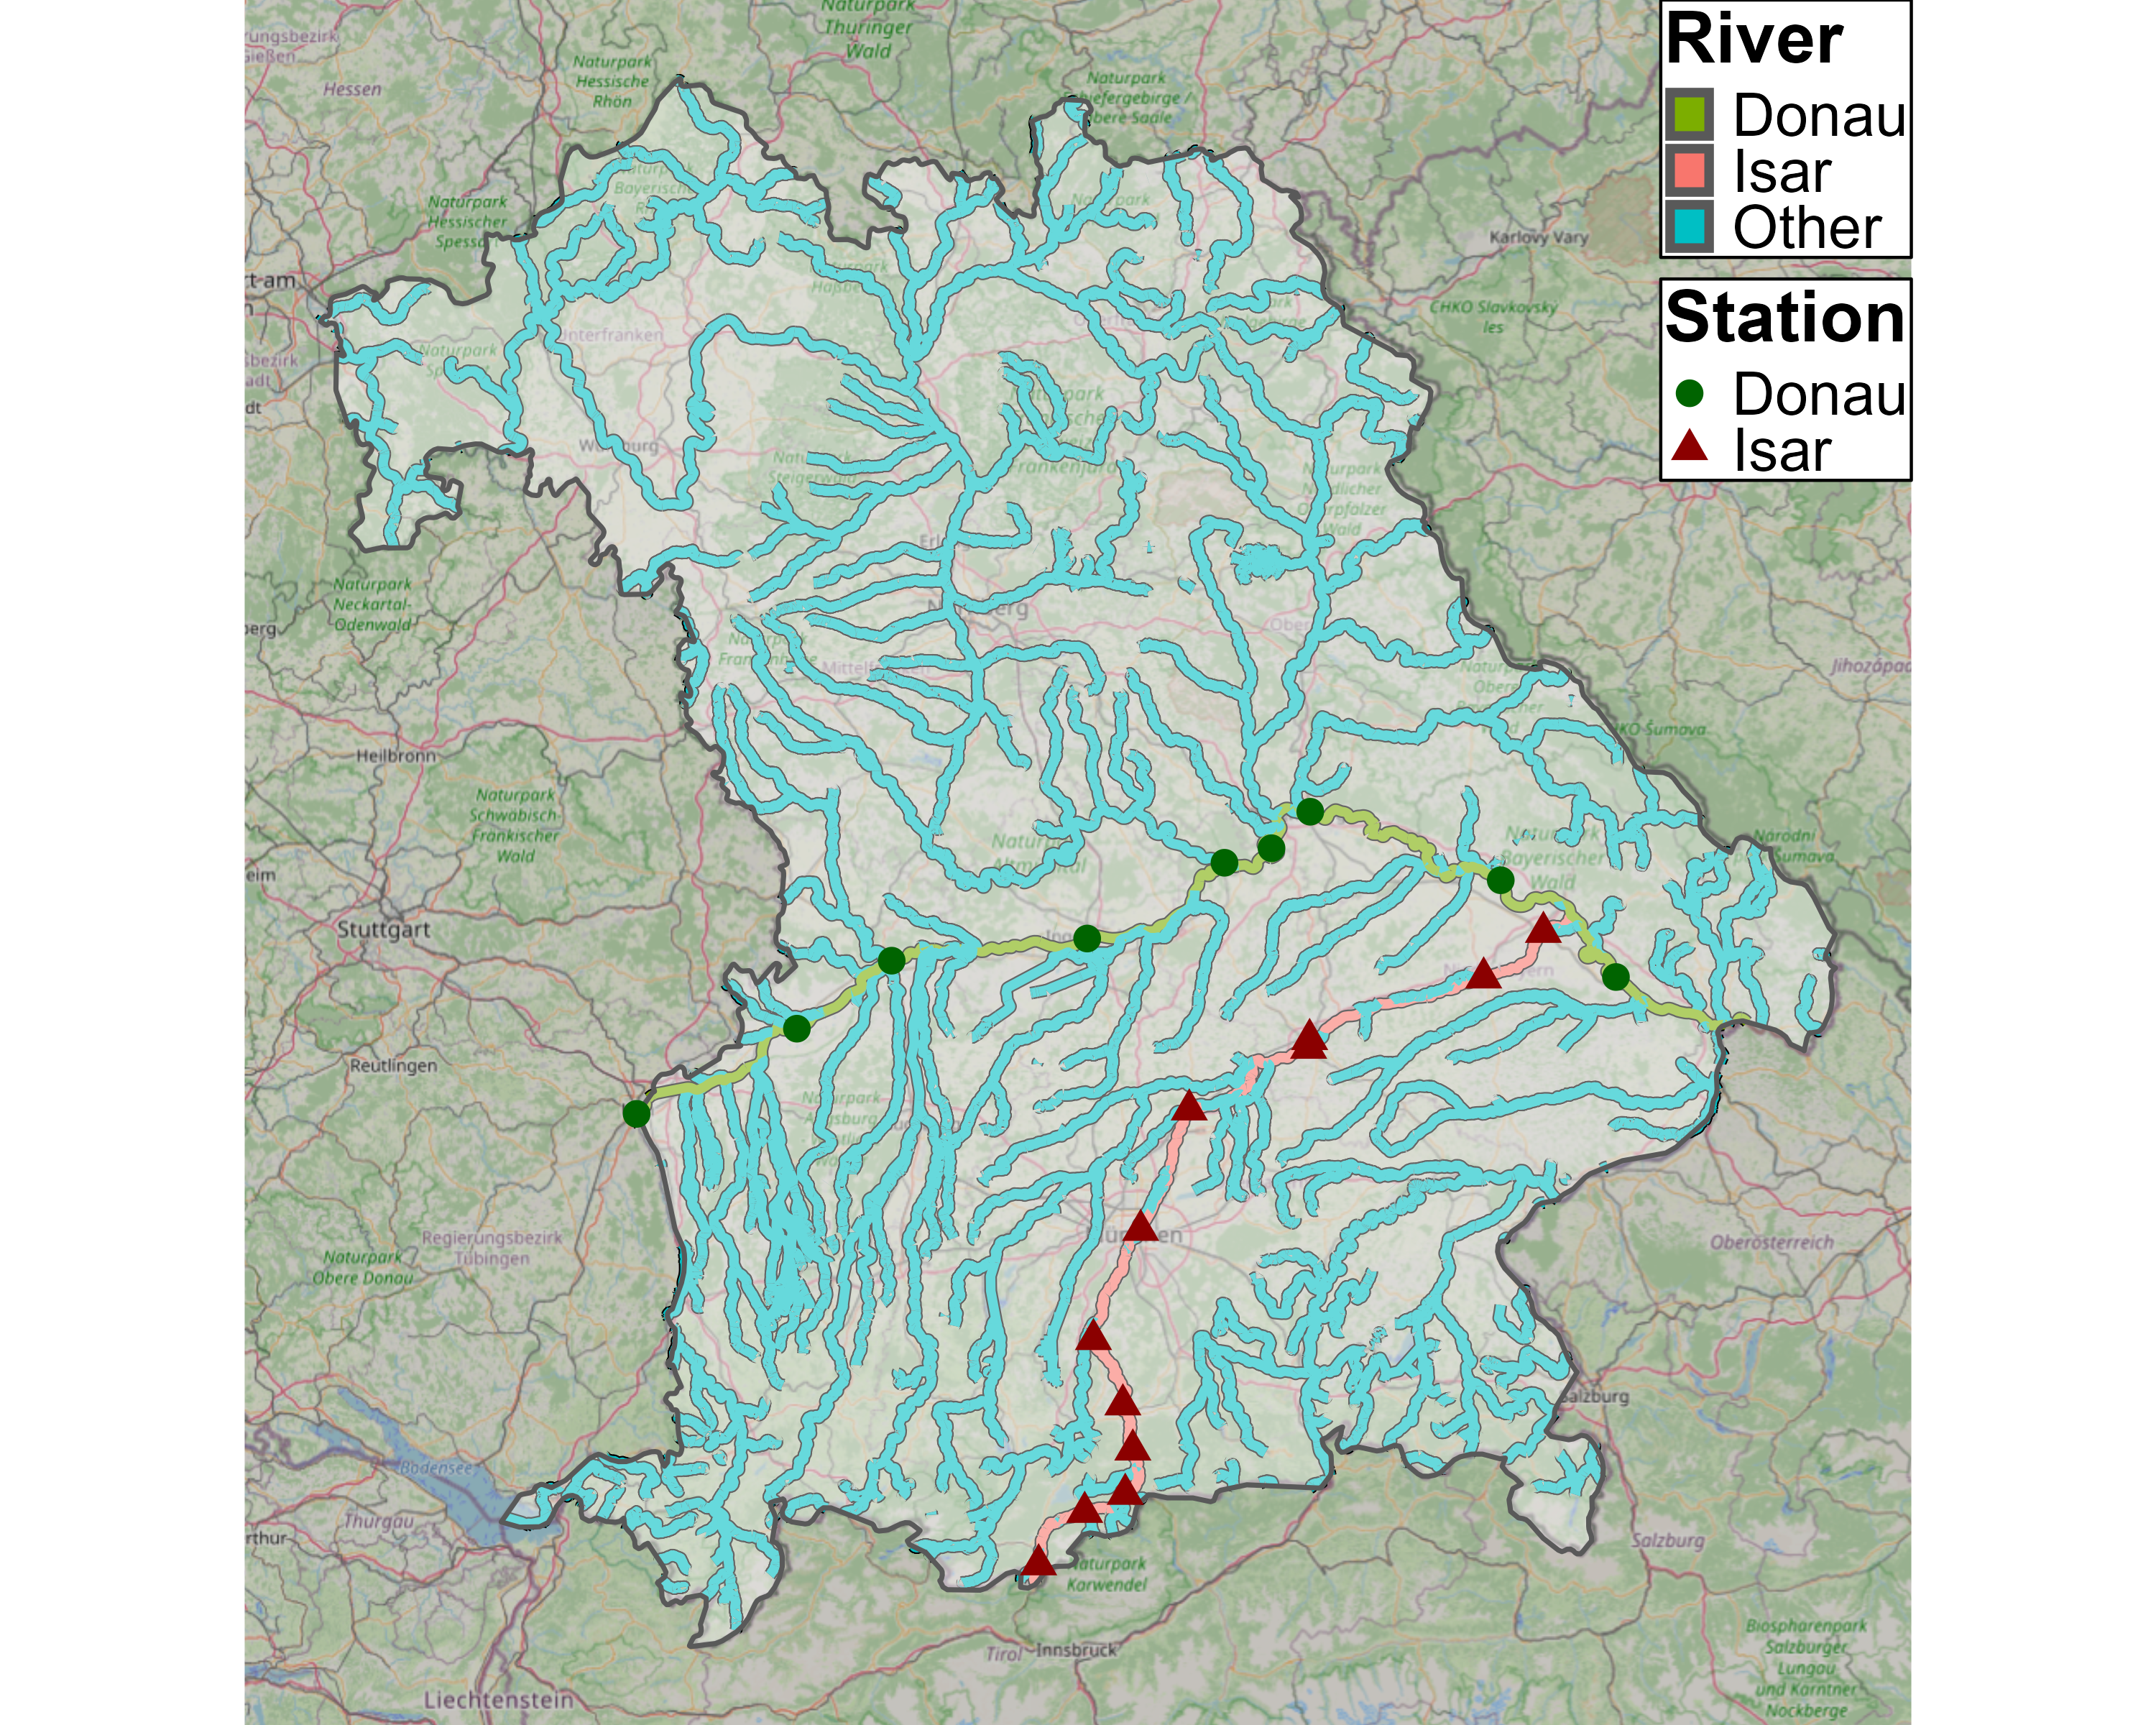
\includegraphics[width=0.7\linewidth]{work/04-floodfreq/figures/data_bavaria_plot} 

}

\caption{The location of the selected measurement stations for the Isar and the Danube in Bavaria.}\label{fig:bavaria}
\end{figure}

Given the annual discharge data for all these stations, we require to identify the
most severe flood event within each year which defined as the event with the largest discharge peak.
To stabilize event detection, the following is based on daily average discharge values we
calculated based on the \(15\) minute time intervals in the original data.\\
The flood detection approach proposed by \citet{grimaldi2006} of using the straight-line method based on a fixed threshold
was found to be highly unreliable, but so was a quantile-based straight-line method.
Both approaches exhibit significant uncertainties in identifying flood events,
particularly, they tend to overestimate flood duration.
Instead, we applied
the baseflow methods proposed and implemented by \citet{wasko2025}.
This method relies on the baseflow index (BFI) which is the ratio of the baseflow volume to the volume of streamflow.
A default BFI threshold of 0.5 was used to distinguish events dominated by rapid runoff contributions typically associated with rainfall- or melt-induced flooding.
Exemplary, figure \ref{fig:hydro} shows the hydrograph for the station in Munich in 2024.

\begin{figure}

{\centering \includegraphics[width=0.7\linewidth]{work/04-floodfreq/figures/data_hydrograph} 

}

\caption{An exemplary hydrograph of the Munich station in 2024 (left) with the applied flood detection method (right).}\label{fig:hydro}
\end{figure}

Both subplots in the figure display the same hydrograph, but the right describes the identification of the most
severe flood. First, all flood events are selected. Then, the flood with the largest peak is identified. The
flood duration is based on the previously described process.
Finally, the
variables of interest are determined. That is,
flood peak is the maximum discharge value occurring within the event,
flood duration is the time span measured in days between the start and end of the event, as determined by the BFI threshold crossings.
Flood volume is the cumulative streamflow over the flood duration, representing total discharge volume in \(m^3\).
These are neatly displayed on the left subplot.\\
Now, we come to the most crucial aspect in our data and show that this structure is also found in \citet{grimaldi2006}. That is, fig \ref{fig:corplot} displays the rank correlation coefficient Kendall's \(\tau\)
of every possible combination between the \(3\) variables separated by river.\\

\begin{figure}

{\centering \includegraphics[width=0.7\linewidth]{work/04-floodfreq/figures/data_cor_plot} 

}

\caption{The Kendall's tau coefficients for the three dependency structures of volume, duration and peak for the Isar and the Danube. Black dots mark the respective results found in Grimaldi (2006).}\label{fig:corplot}
\end{figure}

The boxplots in figure \ref{fig:corplot}
are based on the \(9\) and \(12\) stations along each river, respectively, and
depict the \(\tau\) values for the corresponding variable combination seen on the \(x\)-Axis.
The black dots refer to the \(\tau\) values observed by \citet{grimaldi2006}.
Most important here is that none of the boxplots align horizontally. That is, the strength of dependence
differs between all pairs of variables.
Thereby, our data suggests \(3\) distinct dependencies.
This finding is most crucial and, as we will see later on, renders \citet{grimaldi2006} approach infeasible. Because, as seen from the black dots, not only our data suggest \(3\) separate dependence structures, but also the river \citet{grimaldi2006} considered.\\
Also interesting is the exact order of correlation values by each river.
For both rivers, duration and peak always had the lowest correlation value.
For the Danube,
volume and duration are always the variables with the highest correlation with an exception of only one station.
Nevertheless, all these values are quite similar as seen from the width of the boxplot in figure \ref{fig:corplot}.
For the Isar, on the other hand, we observe not only more variation in the correlation
values, but here the most correlated pair tends to be volume and peak. Of the \(12\) stations, \(8\)
had volume and peak to be the pair with the highest correlation.
This emphazises the aforementioned contrasting
hydrological characteristics which are highly relevant for copula modelling and, thereby, for our analysis.\\
Finally, the analysis section utilizes return periods of flood peaks to derive
average discharge values conditioned on a certain peak.
To ensure these are
comparable among stations, they are normalized by the station specific mean and standard deviation.
To now characterize a conditional distribution using our data, we ordered all flood events within each station
by their peak values and then selected the quantiles corresponding to the
return periods \(2, 5, 10, 20\) and \(50\) years.
Thereby, we obtained \(21\) average discharge values for each return period.
Consider figure \ref{fig:condEmpBoxplots} for a visualization.

\begin{figure}

{\centering \includegraphics[width=0.7\linewidth]{work/04-floodfreq/figures/data_condBoxplots} 

}

\caption{The standardizes average discharge values by peak quantiles of the GKD data.}\label{fig:condEmpBoxplots}
\end{figure}

First of all, note that the average discharge values are on the
y-axis ranging from \(-1\) to \(5\). This is due to the
standardization process within each station. The x-axis denotes the
return periods of the peak.
To account for the different structure between rivers, the figure considers them separately.
Thereby, each boxplot in the Danube column is based on \(9\) data points and \(12\) for the Isar where each data
point corresponds to a station.\\
For both subplots, the average discharge increases with an increase in the return period.
However, while the subplot of the Danube suggests a moderate increase in average discharge values,
the Isar has a stark increase. But by the size of the boxplot at return period \(50\), this increase does not
hold for all stations.

\section{Methods}\label{methods_ff}

To address the dependence structures identified in the previous section,
this chapter
extends the approach of \citet{grimaldi2006} by incorporating vine copulas.
This extension is necessary because a simpler approach is insufficient to capture the full correlation pattern
observed in the data.
The following introduces the foundational theory of copulas,
the family of Archimedean copulas as well as nested Archimedean and vine copula models.
In addition, methods for copula fitting and model selection are briefly discussed.
Then, some applied, but non-essential methods are briefly established.
Together, these elements form the theoretical framework on which this paper is based.
Finally, a few words to the implementation of these methods and used packages.

\subsection{Copulas}\label{cops}

\citet{zhang2019} (p.~62) describe a copula as a cumulative distribution
function (CDF) with standard uniform margins. The dimension \(d\) of a copula
denotes the number of random variables it relates and, hence, a copula is at least bivariate (\(d \geq 2\)).
To give a mathematical definition, consider the vector
\(u = (u_1, ..., u_d) \in \mathbb{R}^d\) where \(u_j \in [0, 1]\) for
\(j = 1, .., d\). Then, a \(d\) dimensional copula is defined by
\citet{durante2016} (p.~14) as function \(C:[0,1]^d\to [0,1]\) if, and only if,
the following conditions hold:\\
i) \(C(u_1, ..., u_d) = 0\) if \(u_j = 0\) for at least one
\(j \in \{1,…,d\}\).\\
ii) \(C(1, 1, ..., 1, u_j, 1, ..., 1) = u_j\).\\
iii) \(C\) is \(d\)-increasing.\\
According to \citet{nelsen2006} (p.~9), condition i) shows that copulas
are grounded. In this context, grounded means that
plugging in \(0\) for just one of the variables yields a copula value of \(0\), independent of the
other variables' value.
The author also mentions that, using condition ii), the margins of the function \(C\) with respect to a certain variable are obtained by
plugging in \(1\) for all other variables.
Finally, the condition of \(C\) to be \(d\)-increasing is cumbersome to map out in
higher dimensions, which is why the following is restricted to the \(d = 2\) case.
According to \citet{nelsen2006} (p.~8), the copula function \(C\) is
\(2\)-increasing if for all \(u_1, u_2, v_1, v_2 \in [0,1]\) with
\(u_1 \leq u_2\) and \(v_1 \leq v_2\):\\
\[
C(u_2, v_2) - C(u_2, v_1) - C(u_1, v_2) + C(u_1, v_1) \geq 0
\label{eq:twoincreasing}
\]
Simply put, 2-increasing means that the volume under the copula density
function over the rectangle \([u_1, u_2] \times [v_1, v_2]\) is
non-negative. This interpretation follows from the fact that copula functions are defined as CDF and holds for higher dimensions, too.\\
The next section introduces the central theorem in copula theory and also derives the already mentioned copula density.

\subsection{Sklar's Theorem}\label{sklarstheorem}

Sklar's Theorem is central to the theory of copulas as it proves
that any multivariate distribution can be constructed using copulas
(\citet{nelsen2006} p.~17, \citet{durante2016} p.~42). Thereby, this theorem allows
to separate the representation of the dependence structure and marginal
distribution functions. The theorem is given by \citet{nelsen2006} (p.~18):\\
Let \(F_{1,..,d}\) be a \(d\)-dimensional joint distribution function with
univariate margins \(F_1, ..., F_d\). Then, there exists a \(d\)-dimensional
copula \(C\) such that\\
\[
F_{1, ..., d}(x_1, ..., x_d)  = C(F_1(x_1), ..., F_d(x_d)) = C(u_1, ..., u_d)
\label{eq:sklar}
\]
where \(u_i = F_i(x_i)\). Also, \(C\) is unique if \(F_1, ..., F_d\) are continuous.
Equation \eqref{eq:sklar} allows \(2\) important conclusion: One,
any multivariate CDF may be expressed as a composition of a copula
function \(C\) and the univariate margins \(F_1, ..., F_d\). Thereby,
\citet{zhang2019} (p.~66) conclude that \(C\) connects the multivariate CDF to
its margins which allows to separately consider marginal and
joint behavior of variables. That is, the problem of determining any
multivariate CDF is reduced to determining the copula. And two, the
marginal distributions do not need to be of the same family because
Sklar's theorem holds regardless.\\
The aforementioned copula density function is given by (see
\citet{zhang2019}, p.~66):\\
\[
c(u_1, ..., u_d) = \frac{\partial C(u_1, ..., u_d)}{\partial u_1 ... \partial u_d} = \frac{f(x_1, ..., x_d)}{\Pi_{i = 1}^df_i(x_i)}
\label{eq:copulapdf}
\]
where \(f(x_1, ..., x_d)\) denotes the joint density of \(X_1, ..., X_d\)
and \(f_i(x_i)\) the marginal density of \(X_i\) for
\(i = 1, ..., d\). Based on this equation, the joint density in terms of the copula density is given by\\
\[
f(x_1, ..., x_d) = c(u_1, ..., u_d)\Pi_{i = 1}^df_i(x_i)
\label{eq:marginalpdf}
\]

\subsection{Symmetric Archimedean copulas and generator functions}\label{archcops}

As Nelsen (p.~109) states, symmetric Archimedean copulas (SACs) are
widely applied due to their large variety and easy construction. However, SACs only allow the same
dependence strength and structure among all possible pairs of variables as \citet{zhang2019}
(p.124) point out. Therefore, they are not suitable for our analysis as concluded from figure \ref{fig:corplot} which suggested \(3\) distinct correlation values.
However, SACs remain an important building block for more complex copula models.
Thus, this section introduces the concept of a generator function as it determines the family a SACs belongs to.
Then, we specifically focus on bivariate SACs because following models are based on these.

We first give the general idea of a generator, then the
representation of a copula in terms of the generator and in the end the
copula families we use for our analysis.\\
\citet{nelsen2006} (p.~110, 111) defines a generator to be a
continuous and strictly decreasing function
\(\phi: [0, 1] \to [0, \infty)\) such that \(\phi(1) = 0\).
If \(\phi(0) \to \infty\), the generator is considered to be strict.
The inverse \(\phi^{-1}:[0, \infty) \to [0, 1]\) of such generators is
strictly decreasing on \([0, \phi(0)]\).
We only apply strict generators as seen towards the end of this section.\\
For a generator to yield a valid \(d\)-dimensional copula,
\citet{grimaldi2006} and \citet{zhang2019} (p.~124) mention that the inverse
requires to be completely monotone which is given if it has
derivatives of all orders with alternating sign\\
\[
(-1)^k \frac{d^k \phi^{-1}(t|\theta)}{dt^k} \geq 0.
\label{eq:changingsign}
\]
Now, we are in the position to formulate the general representation of a
\(3\)-dimensional SAC in terms of its generator.
The relation is given by
\citet{zhang2019} (p.~123) as\\
\[
C(u_1, u_2, u_3 \mid \theta) = \phi^{-1} \left( \phi(u_1 \mid \theta) + \phi(u_2 \mid \theta) + \phi(u_3 \mid \theta) \,\middle|\, \theta \right).
\label{eq:generatorSAC}
\]\\
Equation \eqref{eq:generatorSAC} shows that
SACs are uniquely defined by their generator
function and a parameter vector \(\theta\) which we introduce next.
As mentioned by \citet{nelsen2006} (p.~110, 111, 114), the
assumed functional form of the generator translates to a specific copula
family. Or, vice versa, assuming a copula family implies assuming a specific generator function.
The \(\theta\) vector, on the other hand,
influences the dependence strength within the assumed copula family
as seen in \citet{zhang2019} (p.~86).
This parameter vector takes on an important role in fitting a copula to observed data.
That is, for an assumed copula family, this parameter vector remains to be estimated from the data.
The exact approach is further discussed in section \ref{est}.
For now, note that we focus on the \(3\) generator functions with a one-dimensional \(\theta\) vector.
These are specified in table \ref{tab:generators}.

\begin{longtable}[]{@{}
  >{\raggedright\arraybackslash}p{(\columnwidth - 6\tabcolsep) * \real{0.2542}}
  >{\raggedright\arraybackslash}p{(\columnwidth - 6\tabcolsep) * \real{0.2881}}
  >{\raggedright\arraybackslash}p{(\columnwidth - 6\tabcolsep) * \real{0.2881}}
  >{\raggedright\arraybackslash}p{(\columnwidth - 6\tabcolsep) * \real{0.1695}}@{}}
\caption{\label{tab:generators} Generator functions of selected Archimedean copulas according to \citet{zhang2019} (p.~130) and tail dependencies according to \citet{zhang2019} (p.~132).}\tabularnewline
\toprule\noalign{}
\begin{minipage}[b]{\linewidth}\raggedright
Copula Family
\end{minipage} & \begin{minipage}[b]{\linewidth}\raggedright
Parameter \(\theta\)
\end{minipage} & \begin{minipage}[b]{\linewidth}\raggedright
Generator Function \(\phi(t)\)
\end{minipage} & \begin{minipage}[b]{\linewidth}\raggedright
Tail Dep.
\end{minipage} \\
\midrule\noalign{}
\endfirsthead
\toprule\noalign{}
\begin{minipage}[b]{\linewidth}\raggedright
Copula Family
\end{minipage} & \begin{minipage}[b]{\linewidth}\raggedright
Parameter \(\theta\)
\end{minipage} & \begin{minipage}[b]{\linewidth}\raggedright
Generator Function \(\phi(t)\)
\end{minipage} & \begin{minipage}[b]{\linewidth}\raggedright
Tail Dep.
\end{minipage} \\
\midrule\noalign{}
\endhead
\bottomrule\noalign{}
\endlastfoot
Clayton & \(\theta \in [-1, \infty)\setminus\{0\}\) & \(\phi(t|\theta) = \frac{1}{\theta}(t^{-\theta} - 1)\) & Lower \\
Gumbel-Hougaard & \(\theta \in [1, \infty)\) & \(\phi(t|\theta) = (-\ln t)^\theta\) & Upper \\
Frank & \(\theta \in (-\infty, \infty)\setminus\{0\}\) & \(\phi(t|\theta) = -\ln \left( \frac{e^{-\theta t} - 1}{e^{-\theta} - 1} \right)\) & None \\
\end{longtable}

Finally, equation \eqref{eq:generatorSAC} shows that the arguments
to the SAC are exchangeable (see \citet{nelsen2006} (p.~38)).
Exchangeability is a form of symmetry and implies that the copula treats
all its arguments the same.
Thereby, this representation displays the aforementioned restriction of SACs being able to only depict one unique dependence structure.

\subsection{Taildependence and Rotation}\label{taildep}

After explaining what it means for a copula to be of a certain family,
the following introduces the family specific concept of tail dependence.
Also, we briefly explain how copulas are manipulated to extend the possible dependence structure one family
captures.

Tail dependence is differentiated into upper and lower tail dependence.
Their formulas are given by \citet{czado2019} (p.~34 - 35) as\\
\[
\lambda^{\text{upper}} = \lim_{t \to 1^{-}} \mathbb{P}\left( X_2 > F_2^{-1}(t) \,\middle|\, X_1 > F_1^{-1}(t) \right) = \lim_{t \to 1^{-}} \frac{1 - 2t + C(t, t|\theta)}{1 - t}
\label{eq:uppertaildep}
\]
and\\
\[
\lambda^{\text{lower}} = \lim_{t \to 0^{+}} \mathbb{P}\left( X_2 \leq F_2^{-1}(t) \,\middle|\, X_1 \leq F_1^{-1}(t) \right) 
= \lim_{t \to 0^{+}} \frac{C(t, t|\theta)}{t}.
\label{eq:lowertaildep}
\]
As seen from both equations, tail dependence is defined as conditional probability that both variables are above
or below a threshold quantile.
Thereby, tail dependence
measures how likely it is for both random variables to jointly exhibit extreme behavior.
However, upper tail dependence refers to both variables attaining large values while lower tail dependence means
both variables are jointly small.
Note that both, upper and lower tail dependence, depend on the copula function \(C\) and parameter \(\theta\) and, thus, on the copula
family. The tail dependencies implied by the copula families we consider are also listed in
table \ref{tab:generators} as stated in \citet{zhang2019} (p.~132).\\
Finally, tail dependence is a family specific property, however, a copula function may be rotated to
change its native tail dependence behavior.
Following \citet{pan2024}, this is done by modelling \(u_i' = 1 - u_i\) instead of \(u_i\) itself.
Every such transformation concludes in a \(90\) degree rotation of the copula function in the corresponding
direction. This approach is based on the definition of the copula function as multivariate CDF.
Because if instead of \(u_i\) the transformation \(u_i'\) is modelled,
the probabilistic statement of the copula in the continuous case changes to
\(C(u_1', u_2|\theta) =  \mathbb{P}(X_1 \geq x_1,X_2 \leq x_2)\) and
\(C(u_1, u_2'|\theta) =  \mathbb{P}(X_1 \leq x_1,X_2 \geq x_2)\), respectively.

\subsection{Fully Nested Archimedean copulas}\label{nacs}

Fully nested Archimedean copulas (FNACs) build upon SACs
and partially alleviate their restrictions.
Note that these are the models \citet{grimaldi2006} made extensive use of.\\
As our analysis applies to the trivariate case, FNACs and vines in section \ref{vines} are introduced
for this trivariate case only.

FNACs are built by nesting bivariate SACs\\
\[
C(u_1, u_2, u_3 \mid \theta) = C_1\left( C_2(u_1, u_2 \mid \theta_2), u_3 \mid \theta_1 \right),
\label{eq:defFNAC} 
\]
where \(\theta_1\) and \(\theta_2\) are the parameters corresponding to copula function \(C_1\) and \(C_2\) and
\(\theta = (\theta_1, \theta_{2})\) is a vector containing all parameters.
Note that there are only \(2\) distinct parameters \(\theta_i\) which is why FNACs, in the trivariate
case, are only able to capture \(2\) distinct dependence structures.
This allows \(2\) conclusions. First, partial exchangeability remains which means that
within the bivariate nested copulas \(C_2\), the two arguments \(u_1, u_2\) are
interchangeable (see \citet{embrecht2003} p.~375). So to a degree, symmetry
prevails.
And second, the nested variables \(u_1, u_2\) have the same marginal relation with \(u_3\).
That is, \(C(a, 1, u_3|\theta) = C(1, a, u_3 | \theta) = C_1(a, u_3|\theta_1)\).
In essence, the statements are equivalent but the important take away is that FNACs are not
able to display \(3\) distinct dependence structures. Thereby, they are not suitable for our analysis.
As also \citet{grimaldi2006} observed \(3\) distinct correlations, their results are questionable for the same reason.\\
Additionally to this restriction, \citet{hofert2016} mention that FNACs
require the sufficient nesting condition to be fulfilled for equation \eqref{eq:defFNAC} to yield a valid copula.
We limit our considerations to FNACs where all nested copulas are of the same family.
This corresponds to what \citet{grimaldi2006} used in their analysis.
Then, the sufficient nesting condition is fulfilled if
deeper nested variables have a stronger degree of dependence, i.e.~\(\theta_1 \leq \theta_{2}\).
(see \citet{grimaldi2006}).\\
Note that equation \eqref{eq:defFNAC} may also be represented in terms of the generator function. Thereby, additional requirements
regarding the composition of generator functions emerge, as mentioned by \citet{zhang2019} (p.~174).
However, discussing these requirements is beyond the purpose of this paper. The interested reader is refered to \citet{zhang2019} (p.~174).

\subsection{Vine Copulas}\label{vines}

Vine copulas use the pair-copula construction (PCC) explained by \citet{czado2019} (p.~77 - 80) to characterize
multivariate dependence structures.
That is, PCC decomposes multivariate densities into products of (conditional) bivariate densities (see \citet{czado2019} p.~88).\\
There exist multiple vine copula classes, depending on the structure the PCC implies, but as we are concerned with the trivariate case,
these constructions are equivalent.

We use \citet{czado2019} (p.~78, 90) and define the trivariate copula density as\\
\[
c_{123}(u_1, u_2, u_3|\theta) = c_{12}(u_1, u_2|\theta_{12}) \cdot  c_{23}(u_2, u_3|\theta_{23})  \cdot c_{13|2}(u_1|u_2, u_3|u_2\mid \theta_{13|2})
\label{eq:simpvinecopdf}
\]
where \(u_i|u_j = F_{i|j}(x_i|x_j)\) denotes the conditional probability.
Note that this copula density is based on the simplifying assumption for vines (\citet{czado2019} p.~90, \citet{nagler2018}) which means
that the conditional bivariate density \(c_{13|2}\) is independent of exact \(x_2\) values.
It only depends on the conditional probabilities.\\
Visible from the number of parameters in the \(\theta\)-vector, vines are able to capture all \(3\) distinct
dependence structures in the trivariate case.
Also, in contrast to FNACs from section \ref{nacs} where we followed \citet{grimaldi2006}, we do not require the bivariate copulas to be of the same family. Thereby,
not only the strength of dependence between all \(3\) variables may differ, also
the dependence structure is allowed to change from pair to pair.

\subsection{Estimation and Selection Process}\label{est}

In practice, we need not only to estimate the parameter vector \(\theta\), but also select the best fitting copula.
Thus, the following briefly introduces the pseudo maximum likelihood (ML) approach.
Also, we give a reminder on the Akaike Information Criterion (AIC) as it is our information criterion of choice to select a copula model.

To avoid assumptions on the marginal distributions,
we estimate the parameter vector \(\theta\) using the pseudo-likelihood proposed by \citet{genest1995}\\
\[
\hat{\theta} = argmax_\theta\ l(\theta) = argmax_\theta\ \sum_{k = 1}^{n}log[c(u_{1k}, u_{2k}, u_{3k}|\theta)],
\label{eq:pseudologlik}
\]
where \(u_{ik}\) denotes the marginal empirical distribution function scaled by \(\frac{n}{n+1}\).
These transformed variables are refered to as pseudo-observations.
Depending on the copula model, the definition of the copula density follows either from
equation \eqref{eq:defFNAC} or \eqref{eq:simpvinecopdf}.
Thus, the exact estimation process slightly differs between copula models.\\
The AIC is given by \citet{fahrmeir2013} (p.~164) as\\
\[
AIC = -2 l(\hat{\theta}) + 2 (|M| + 1)
\label{eq:AIC}
\]
where \(l(\hat{\theta})\) represents the log-likelihood of the copula model fit and \(|M|\) the number of parameters included in the model.
We select that copula model with the smallest AIC.

\subsection{Identifying univariate margins}\label{gev}

While the the estimation process described in section \ref{est} utilizes the
empirical distribution function, an empirical function has undesired properties when re-transforming copula data.
That is, during the estimation process, the empirical distribution functions ensures we
do not affect the copula model fit by missspecifying the marginal distributions.
However, after fitting the copula, whenever the inverse of the empirical distribution is applied, it bins any continuous data because it is a step-wise function. This, of course, limits the power of our copula analysis.
Thus, we decided to fit a Generalized Extreme Value (GEV) distribution to the marginal distribution only for re-transforming any results from the fitted copula models.
The distribution function for the GEV family is given by \citet{coles2001} (p.~47)\\
\[
G(z) = \exp\left\{ -\left[ 1 + \xi \left( \frac{z - \mu}{\sigma} \right) \right]^{-1/\xi} \right\},
\]
defined for \(\left\{ z \middle| 1 + \xi \left(\frac{z - \mu}{\sigma}\right) > 0 \right\}\) where
\(-\infty < \mu < \infty\) denotes the location parameter,
\(\sigma > 0\) the scale parameter and
\(-\infty < \xi < \infty\) the shape parameter.
In practice, these parameters are usually unknown, but \citet{coles2001} (p.~50) describes how these parameters are estimated from data using the ML approach.\\
Since GEV distributions are not at essence for our work, we refer the interested reader to \citet{coles2001} (chapter 3)
for a more detailled consideration.

\subsection{\texorpdfstring{Kendall's \(\tau\)}{Kendall's \textbackslash tau}}\label{kendallstau}

According to \citet{kendall1990} (p.~6), \(\tau\) is a measure of association
between two random variables that distinguishes concordant and
discordant pairs. Concordance means that the two variables move in the same
direction while discordance means moving in opposite directions.\\
\citet{zhang2019} (p.~86) and \citet{nelsen2006} (p.~159,
161 - 164) show that Kendall's \(\tau\) is directly connected to the generator function and, thus,
a function in the parameter \(\theta\).\\
\[
\tau(t)= 4 \int_0^1 \frac{\phi(t|\theta)}{\phi'(t|\theta)}dt + 1
\label{eq:cKendall}
\]
where \(\phi'(t|\theta)\) denotes the derivative of the generator function. Note that this relation is positive
which is seen in \citet{zhang2019} (p.~134). That is, if the parameter of copula increases, the strength of dependence
increases. Vice versa, if correlation increases, \(\theta\) increases, too. Also, note that this implies that
estimating a \(\theta\) implicitly estimates a \(\tau\) value.
This is a relation we will use during our simulation.\\
Empirically, there are multiple versions of Kendall's \(\tau\) depending
on the data structure. Since this paper focuses on continuous variables
only, the formula given by \citet{kendall1990} (p.~5) is applicable\\
\[
t = \frac{P-Q}{\frac{1}{2}n(n-1)}.
\label{eq:eKendall}
\]
\(P\) denotes the number of concordant and \(Q\) the number of
discordant pairs in the data.

\subsection{Software}\label{software}

The whole analysis is implemented using the programming language R.
We used the \texttt{hydroEvents} package by \citet{wasko2025}.
This method relies on the BFI as explained in the data section using a deftault BFI of \(0.5\).
Additionally, the \texttt{eventBaseflow} function calculates the BFI at each time step and extracts discrete flood events when the BFI falls below the specified threshold for a user-specified minimum duration.
For copulas, we relied on the \texttt{copula} package by
\citet{hofert2025} and the \texttt{pobs} function to apply the empirical distribution function as described in section \ref{est}.
FNACs are dealt with using the
\texttt{HAC} by \citet{okhrin2014}, especially the
function
\texttt{estimate.copula} for FNAC fitting which implements the ML approach from section \ref{est}. This required
some additional code to select the best fitting copula according to the AIC.
For vine copulas,
\texttt{VineCopula} package by \citet{nagler2024} was consulted.
Especially the function
\texttt{RVineCopSelect} which implicitly fits a selection of copulas and also selects the one with the smallest AIC.
Finally, GEV distribution were fitted using the function
\texttt{fevd} from the
\texttt{extRemes} package by \citet{gilleland2016} which uses MLE to determine the parameters mentioned in \ref{gev}.

\section{Simulation}\label{sim}

To examine the incapability of FNACs to capture \(3\) distinct dependence structures in a trivariate
setting, we ran a simulation.
The true underlying model builds a vine copula models.
This section is limited to the most crucial finding
which is highly relevant for the interpretation of our results in the following section.

We set up the simulation by drawing \(27000\) random samples of size \(15, 30, 50, 1000\).
The sample size of \(50\) represents our real world conditions while \(1000\) observations aim to examine large sample behavior. The two smaller samples sizes are interesting because we earlier decided to remove stations due to their small
sample size.\\
For each drawn sample,
the underlying vine copula model has \(2\) wheels to tweak:
First, each copula density
of the underlying vine copula model is allowed to be of one of the copula families
listed in table \ref{tab:generators} leading to a possible total of \(3^3 = 27\) copula family combinations.
Second, we allowed for \(4\) different correlation values, \(2\) of which correspond to the observed average
correlation values in the Isar and the Danube. The remaining \(2\) aimed to examine general behavior of FNACs. That is, we added a Low-Medium-High (LMH) correlation structure with correlation values of \(0.1, 0.5, 0.85\) and a
Low-High-High (LHH) structure using \(0.1, 0.8, 0.8\).\\
Thereby, we had \(27000\) data points per sample size which are split among all \(27\) possible copula family combinations
and \(4\) possible correlation structures. This leads to roughly \(\frac{27000}{4\cdot 27} = 250\) data points per setup.
It is not exactly \(250\) because we used a uniform draw to select copula families and correlation
structure as it drastically simplified implementation.\\
The one result we want to focus on is described in figure \ref{fig:simresults}.

\begin{figure}

{\centering \includegraphics[width=0.9\linewidth]{work/04-floodfreq/figures/sim_NAC_if_Vine_DPG} 

}

\caption{The simulation results by sample size and correlation structure.}\label{fig:simresults}
\end{figure}

This figure uses multiple subplots displaying trace plots of the \(\tau\) values estimated by the FNAC model.
Kendall's \(\tau\) estimates are displayed on the y-axis while the index
of the iteration in which this model was fitted is on x-axis. Note that this plot does not differ by
copula family combination leading to roughly \(\frac{27000}{4} = 6750\) iterations each.
The black lines in each subplot refers to the true underlying correlation values.
The name of the corresponding
correlation structure is to the right hand side of the plot.
Additionally, the figure is divided by the sample size on which the estimated FNAC model is based on. From a
sample size of \(15\) on the left up to a size of \(1000\) on the right.
Color-wise, the red line refers to the \(\hat{\tau}\) of the nested FNAC and the blue line to the outer estimate.
Due to the sufficient nesting condition (see section \ref{nacs}), the inner \(\hat{\tau}\) in each iteration is always larger than the outer.\\
The first observation is the decrease in variance of the estimators as the sample size increases. This holds for
all possible correlation structures and was expected.
Now, focus only on the column of sample size \(1000\). Especially in the Low-Medium-High subplot,
we observe that the inner \(\tau\) estimate moves around the most upper black line.
Thereby, the nested copula in a FNAC correctly captures the largest correlation value.
The blue line, however, moves around the second largest black line and its volatility remains comparably large.
We conclude that, first, the \(\tau\) estimate of the outer copula of a FNAC model varies within a set interval
for large sample sizes. This is similar to what \citet{grimaldi2006} found in their work when they examined
how SACs perform if the true underlying model is a FNAC.
Second, and highly relevant for our analysis,
the \(\hat{\tau}\) based on the outer copula of a FNAC
tends towards the second largest correlation value in the (simulated) data.
This implies that, due to the same copula margins mentioned in section \ref{nacs}, FNACs systematically
overestimate the weakest dependence strength.
This is an important result because it explains not only the comparably bad performance of FNACs during our
application, but also their bias in the results.

\section{Application}\label{app}

Due to our finding during the simulation, we focus on presenting the fitted vine copulas models.
Only for the the model comparison, we jointly consider FNACs and vines to discuss the
effect of the bias in FNACs and its practical meaning.

\subsection{Goodness of Fit}\label{goodness-of-fit}

The following discusses the goodness of fit for the vine copula model
based on the Munich station using figure \ref{fig:visualGoF}.

\begin{figure}

{\centering \includegraphics[width=0.7\linewidth]{work/04-floodfreq/figures/app_visualGOF} 

}

\caption{The contour lines and synthetic data plots for the Munich station.}\label{fig:visualGoF}
\end{figure}

This figure consists of \(6\) subplots.
Each column of subplots refers to a pair of variables specified in the column header.
The variable named first is displayed on the y-axis.
Note that all subplots are on copula level. Thus, all axes range from \(0\) to \(1\).
The top row of subplots shows the contour lines for the fitted copula density and the bottom row a synthetic
random sample from the copula model.
The black points in every subplot depict the pseudo observations of the corresponding variables.\\
Starting with bottom row, a good model fit implies that the light blue points capture the structure
of the pseudo observations.
This seems to be the case for all variable pairs as not only the shape of the black points is nicely
reflected in the synthetic data points, but also the strength of dependence matches.
This is validated when comparing the empirical correlation values with the correlation implied
by the fitted models as seen in table \ref{tab:corrvalues}.
The largest absolute difference between the correlation values is just \(0.02\).

\begin{longtable}[]{@{}
  >{\raggedright\arraybackslash}p{(\columnwidth - 8\tabcolsep) * \real{0.2475}}
  >{\raggedright\arraybackslash}p{(\columnwidth - 8\tabcolsep) * \real{0.2475}}
  >{\raggedleft\arraybackslash}p{(\columnwidth - 8\tabcolsep) * \real{0.1881}}
  >{\raggedleft\arraybackslash}p{(\columnwidth - 8\tabcolsep) * \real{0.1485}}
  >{\raggedleft\arraybackslash}p{(\columnwidth - 8\tabcolsep) * \real{0.1683}}@{}}
\caption{\label{tab:corrvalues} Describtives on the fitted copula model for Munich station.}\tabularnewline
\toprule\noalign{}
\begin{minipage}[b]{\linewidth}\raggedright
Pair
\end{minipage} & \begin{minipage}[b]{\linewidth}\raggedright
Copula Family
\end{minipage} & \begin{minipage}[b]{\linewidth}\raggedleft
Empirical \(\tau\)
\end{minipage} & \begin{minipage}[b]{\linewidth}\raggedleft
Fitted \(\tau\)
\end{minipage} & \begin{minipage}[b]{\linewidth}\raggedleft
\(|\Delta \tau|\)
\end{minipage} \\
\midrule\noalign{}
\endfirsthead
\toprule\noalign{}
\begin{minipage}[b]{\linewidth}\raggedright
Pair
\end{minipage} & \begin{minipage}[b]{\linewidth}\raggedright
Copula Family
\end{minipage} & \begin{minipage}[b]{\linewidth}\raggedleft
Empirical \(\tau\)
\end{minipage} & \begin{minipage}[b]{\linewidth}\raggedleft
Fitted \(\tau\)
\end{minipage} & \begin{minipage}[b]{\linewidth}\raggedleft
\(|\Delta \tau|\)
\end{minipage} \\
\midrule\noalign{}
\endhead
\bottomrule\noalign{}
\endlastfoot
Duration -- Peak & Clayton & 0.15 & 0.16 & 0.01 \\
Peak -- Volume & Gumbel-Hougaard & 0.49 & 0.51 & 0.02 \\
Duration -- Volume & 180° Rotated Gumbel-Hougaard & 0.60 & 0.59 & 0.01 \\
\end{longtable}

Now, consider the top row of figure \ref{fig:visualGoF} in combination with the corresponding copula families
mentioned in table \ref{tab:corrvalues}. The Clayton and 180° rotated Gumbel-Hougaard copula imply
lower tail dependence for the relation between duration and peak as well as duration and volume, respectively.
Thereby, if the flood peak is small, the duration tends to be short, too. Also, the volume of a flood
is more likely to be small
given a short flood duration.
However, due to its small strength of dependence, the tail dependence for duration and peak is rather small.
This is not only suggested by the contour lines,
but follows from the low \(\tau\) value which implies that paramter \(\theta\) is small, too, as mentioned in
section \ref{kendallstau}.
This in turn affects the tail dependence as it is a function in \(\theta\), as discussed in section \ref{taildep}.
Finally, a Gumbel copula is fitted to the peak and volume pair implying upper tail
dependence. Thus, given a large peak, the flood volume tends to be large, too.

\subsection{Fitted Tail Dependencies}\label{fitted-tail-dependencies}

Because tail dependence is an important concept from a hydrological point of view,
we extend the tail dependence analysis from the previous section to all considered stations.

Contemplate figure \ref{fig:bavariaTaildep} for a visual assessment of the tail dependence structure.

\begin{figure}

{\centering 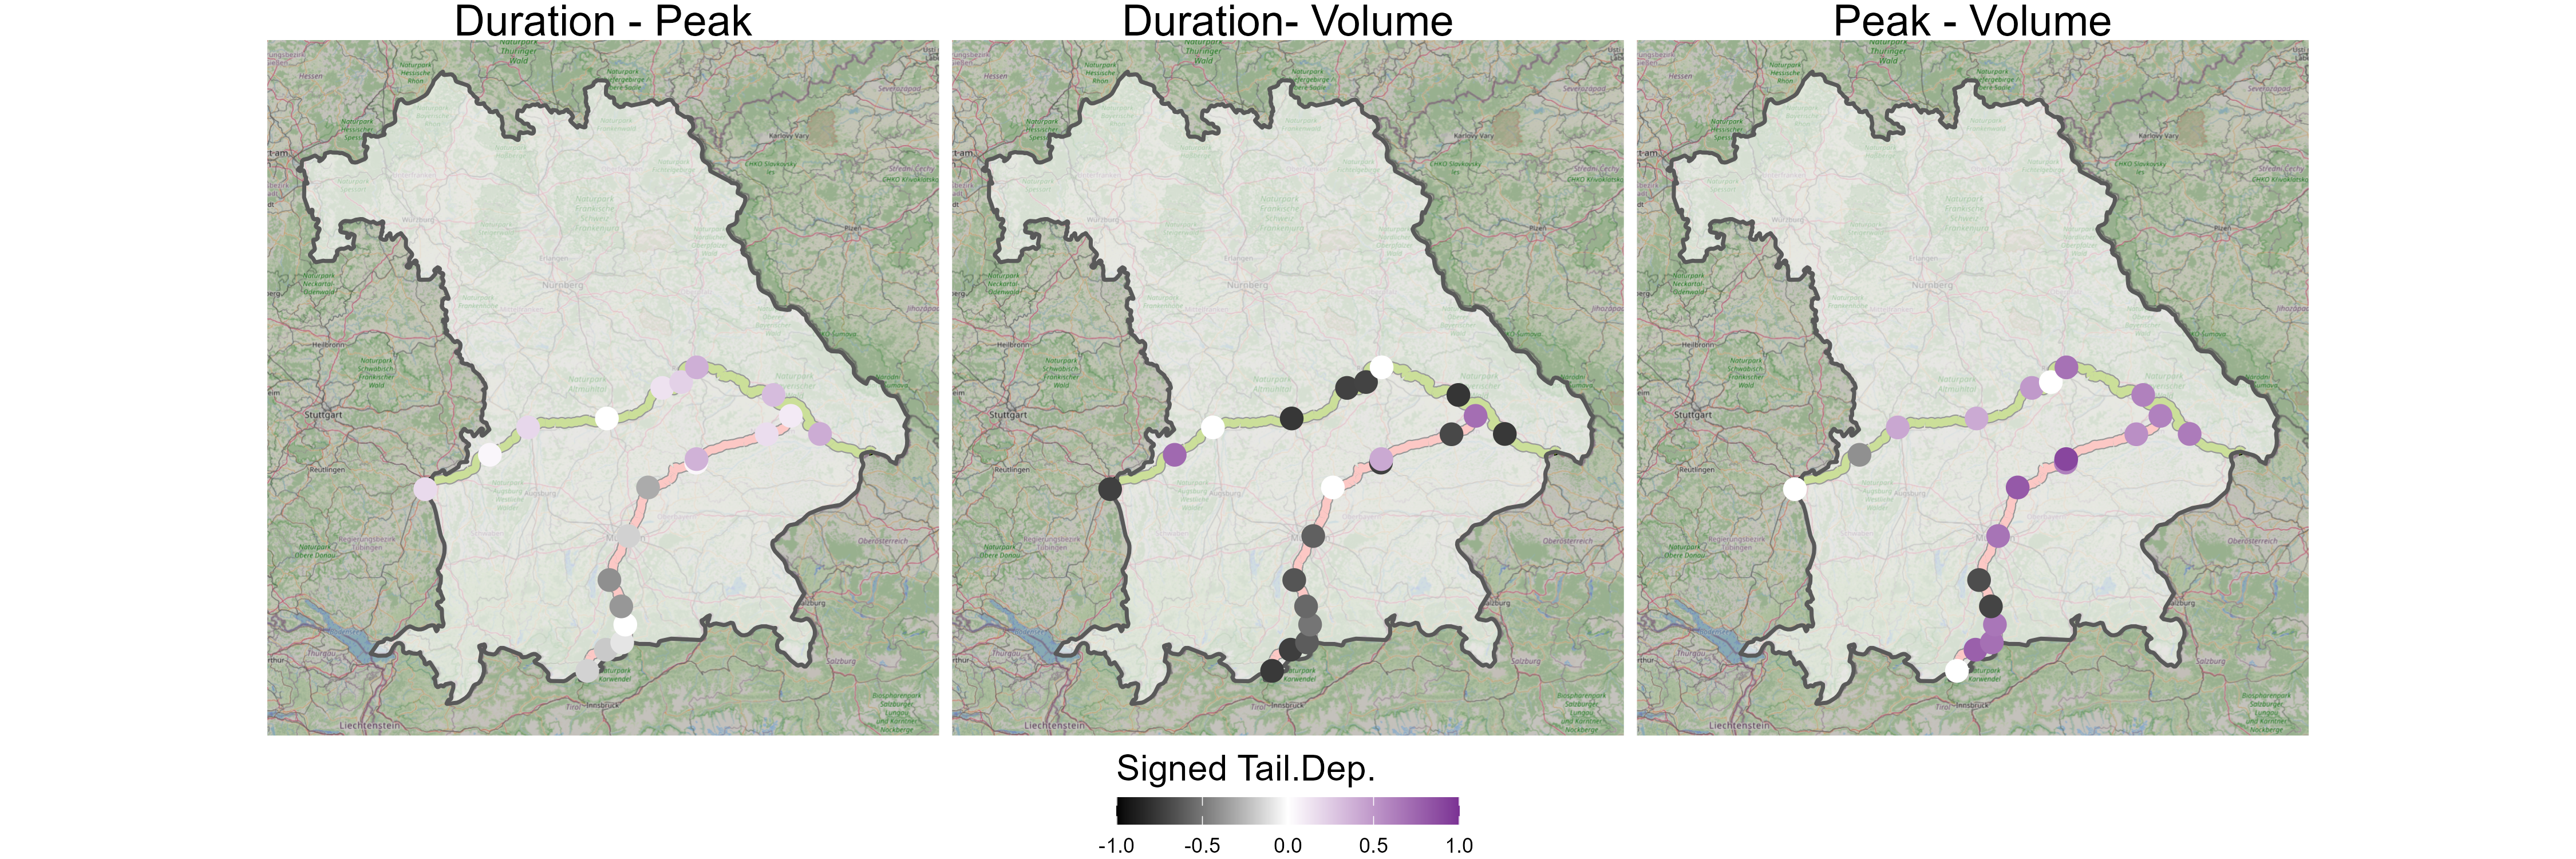
\includegraphics[width=0.7\linewidth]{work/04-floodfreq/figures/app_bavaria_taildep} 

}

\caption{The signed tail dependencies of the three variable combinations.}\label{fig:bavariaTaildep}
\end{figure}

This plot shows \(3\) different subplots, one for each variable pair.
The subplots are based on figure \ref{fig:bavaria} and display all stations colored by their
tail dependence value.
Because we only allowed for copula families with either upper, lower or no tail dependence,
we visualize the signed tail dependence.
That is, upper tail dependence values remain unchanged, but lower tail dependencies are multiplied by
\(-1\). Thereby, the blacker a station is colored in, the stronger the lower tail dependence and the more
purple the stronger the upper tail dependence. A totally white point on the map refers to no tail dependence.
In these cases, a Frank copula has been fitted to the variable pair.\\
In general, we observe lighter colors for the duration-peak pairs which is due to the rather
small correlation values. This follows from the reasoning in the previous section.
Duration and volume exhibit the darkest colors suggesting that if the flood duration is short, the
flood volume tends to be small, too, for the majority of the considered stations.
This is especially the case at the Isar stations. But, the relationship begins to shift towards a positive dependence approximately at the middle of the river, likely due to the influence of tributaries that contribute additional water as the river progresses downstream.
In contrast, the Danube displays mixed signals for the duration-volume pair, indicating a more complex or variable relationship, possibly reflecting the diverse hydrological influences across its larger catchment area.\\
For the peak-volume pair, both rivers show a positive tail dependence, indicating that higher peak flows are generally associated with larger flood volumes. This is consistent with expected hydrological patterns where significant peak events often appear with substantial volumes of water. The duration-peak pair exhibits the weakest tail dependence, suggesting that the flood duration does not strongly influence the peak discharge. This weak correlation is indicative of the more dynamic nature of peak discharges, which may be influenced by short-term, localized weather events rather than the overall duration of the flood.\\
Across all three pairs, the Isar consistently demonstrates more extreme tail dependence trends compared to the Danube. This difference is likely due to the more extreme flood characteristics in the Isar, which are influenced by factors such as snowmelt, topography, and high spring rainfall events (\citet{parajkaa2019}).

\subsection{Event Probability}\label{event-probability}

The following examines the difference between a univariate and the multivariate approach
for flood characterization and thereby addresses one of our research questions.
To answer it, the
following focuses on the flood event in Munich 2024
which had a peak of \(462m^3/s\), took \(20\) days and had a volume of \(406m^3\).

Figure \ref{fig:probUni} displays the marginal fit of a GEV distribution to the peak data for the Munich station.

\begin{figure}

{\centering \includegraphics[width=0.5\linewidth]{work/04-floodfreq/figures/app_univariate_hq} 

}

\caption{The GEV fit for the Munich station. The red area delineates floods with a peak equal or higher to the flood event of 2024.}\label{fig:probUni}
\end{figure}

The x-axis of this plot denotes the peak values, the y-axis the density of the fitted GEV model.
The histogram displays the original data to which the GEV distribution was fitted. The resulting smooth distribution
is marked by the blue line. The red vertical line marks the peak value of \(462m^3/s\) and
the the shaded area visualizes the probability
to observe a peak at least as large. Based on the GEV fit, the probability is calculated to be
\(19\%\). Thereby, this approach assigns the a
return period of such a peak to be \(\frac{1}{0.19} \approx5\) years.
Thus, characterizing the whole flood event only by its peak,
the return period of the whole flood in Munich of 2024 according to the univariate model is \(5\) years.\\
The trivariate copula model allows to also consider volume and duration values to characterize a flood event.
Figure \ref{fig:probMulti} is based on figure \ref{fig:visualGoF} and visualizes
how the multivariate model determines the probability for a flood event to be at least as severe.
Also, this plot helps to understand the quite stark differences in the probabilities.

\begin{figure}

{\centering \includegraphics[width=0.7\linewidth]{work/04-floodfreq/figures/app_multivariate_hq} 

}

\caption{The copula fit for the Munich station. The red area delineates floods with a peak, volume and duration equal or higher to the flood event of 2024.}\label{fig:probMulti}
\end{figure}

Note that, as before, this figure displays the data in terms of their pseudo observations.
The red dot in each subplot marks the event in 2024 and the red lines correspond to the univariate
univariate observed pseudo values.
Thereby, a flood event is at least as severe as the flood in Munich if it lies wihtin the shaded area.
Thus, the probability is obtained by integrating the joint copula density over the cube made
up by the shaded area.
According to our model, this adds up to be \(2.7\%\) which corresponds to a return period of merely \(\frac{1}{0.027} \approx 37\) years.
Thereby, the return period for such an extreme flood is \(\frac{37}{5}\approx7\) times longer
if the flood is characterized not only but its peak, but also by its volume and duration value.
The reason for this drastic difference is
seen in figure \ref{fig:probMulti}. While the pseudo observation
of the peak value of the event is around \(0.76\),
the volume is at \(0.96\). That is, the volume during this flood was exceptionally large which
decreases the
probability of such an event to occure.
Visually, this is seen from the shaded area being very slim.
In contrast, the univariate consideration of
peak values only
is not capable to account for this.

\subsection{Model Comparison}\label{model-comparison}

Finally, this section examines the effect of different peak values onto the other characteristics of a flood.
Mainly, we are interested in the average discharge value during a flood event as it is a measure
of the average energy the system has to deal with.

First, we fit
station specific GEV distributions onto the observed peak values and determine peaks
for the return periods of \(2, 5, 10, 20\) and \(50\) years.
We choose the upper bound of \(50\) years to validate the model predictions using the available data.
Conditional on these peaks, the most likely combination of duration and volume are determined as well as
the average discharge values.
Figure \ref{fig:modelEval} is based on figure \ref{fig:condEmpBoxplots} and displays our results.

\begin{figure}

{\centering \includegraphics[width=0.7\linewidth]{work/04-floodfreq/figures/app_modeleval} 

}

\caption{The model comparison by river between FNACs and vines.}\label{fig:modelEval}
\end{figure}

The rows of the figure refer to the model structure applied to predict the average discharges.
Additionally, we colored each model prediction by which variable pair had the highest correlation.
First, consider the vine model fits in the bottom row. The models
correctly capture the trend suggested by the boxplots independent of which pair of variables has the highest
correlation. For a return period of \(50\), model predictions and boxplots increase in variance.
This is reasonable because the manner in which an event is extreme depends on the station. Thereby, a joint
behavior in boxplot and model prediction suggests a good fit.
For FNACs, consider their performance within the stations of the Isar first. There is a visible
difference in model performance depending on which variable pair has a larger correlation value.
If volume-peak
have a larger correlation value,
the model captures the underlying data structure more reliable than for
volume and duration being stronger correlated pair.
For the Danube, FNAC models barely move at all failing to capture any trend in the data whatsoever.
To quantify the visual analysis, consider the mean absolute difference of the model prediction to the median
of the data: For FNACs, the error for the Danube is
\(0.70\)
and the error for the Isar
\(0.90\)
.
Vine outperformed FNACs with an error of
\(0.35\)
for the Danube and
\(0.53\)
for the Isar.
However,
take these with a grain of salt because especially for a return period of \(50\) years,
we deal with an extreme event.
And it is reasonable to expect extreme events to be highly station specific.
Thereby, a model perfectly predicting the median of the average discharge data is not necessarily desirable.\\
The reason for the underperformance of FNACs is their incapability of capturing \(3\) unique dependence structures
which leads to \(2\) distinct effects.
First and mainly, due to the shared bivariate marginal copula, the performance of FNAC models is
highly impacted by which variable pair is higher correlated. Because by the sufficient nesting condition,
the stronger correlated variable pair is required to build the nested copula.
If duration-volume is the higher correlated pair and, thus, peak in the outer copula,
the dependence between duration-peak and volume-peak is forced to be identical. Thereby, conditioning on
a peak value has the identical effect on both nested variables.
However, if peak is inside the nested copula, duration-peak and volume-peak remain a distinct
relation structure to peak. Thereby, both models are wrong, but one of them remains more flexible.\\
The second effect is independent of the nesting structure. As result of the simulation we observed a systematic
overestimation of the lower correlation value. Because in our data, the smallest correlation
value is always between duration-peak, this strength of dependence is systematically overestimated.
This implies that an increase in peak affect duration more than it should. And because
all observed correlation values between the two variable are positive, the duration of a flood
for given an increasing peak is always overestimated. This implies that the average discharge predicted by
FNACs is systematically too low because the volume is divided by a duration that is too long. In conlusion,
even if some of the FNAC models look as if they captured the underlying structure, they really did not.
Thereby, this application
nicely depicts the shortcomings of FNACs and the reason why they are
not suitable if their assumptions are violated.

\section{Conclusion}\label{conclusion}

The aim of this work was to investigate the potential of copula-based multivariate models for flood risk assessment in Bavaria, focusing on the joint behaviour of flood peak, volume and duration.
Three main research questions were addressed: the applicability of copula models to Bavarian flood data, the comparative performance of NACs and vine copulas, and the impact of using multivariate rather than univariate approaches to estimate return periods.
Our results confirm that copula theory provides a robust framework for modelling the dependence structure between multiple hydrological variables. By applying both vine and FNACs to \(21\) stations, we demonstrated that multivariate models are capable of capturing complex, asymmetric dependencies that are not accounted for in traditional univariate analyses.
A key finding is the spatial variability in tail dependence structures across the study area. The Isar, in particular, exhibited more pronounced and often more extreme dependencies---especially between volume and duration, suggesting stronger hydrological controls related to topography, snowmelt, and spring precipitation patterns.
In contrast, the Danube showed more mixed signals, underscoring the necessity for flexible dependence structures that can adapt to regional hydrological conditions.
When comparing the model structures, vine copulas consistently outperformed FNACs which suffered from structural biases. This limitation was particularly evident when analysing conditional average discharge values, where FNACs systematically underestimated flood severity.
Finally, the comparison of univariate and multivariate return period estimations underscores the need of a multivariate perspective.
For the 2024 Munich flood event, the return period increased from \(5\) to \(37\) years when considering the joint severity of peak, volume, and duration. This highlights the risk of underestimating extreme events when relying solely on univariate peak discharge values.
In conclusion, the integration of flexible multivariate copula models, especially vine copulas, represents a significant advancement in flood risk analysis. Their ability to capture spatial and structural dependencies can greatly improve the reliability of flood risk assessments and help create more resilient flood management strategies in Bavaria.

\chapter{Mapping of Potential Natural Vegetation with Machine Learning Methods}\label{mapping-of-potential-natural-vegetation-with-machine-learning-methods}

\emph{Author: Elena Pellerano \& Julius Weiss }

\emph{Supervisor: Henri Funk}

\section{Abstract}\label{abstract-4}

Climate change is expected to significantly affect the distribution of vegetation across Europe. Traditionally, such questions are addressed by classical ecological inference at small spatial scales or by process-based Dynamic Global Vegetation Models (DGVMs). Following and replicating the data-driven approaches of \citet{hengl2018} and \citet{bonannella2023}, this study implements a random forest model to predict the spatial distribution of European biomes using a historical pollen dataset and environmental covariates (climate and topography). In addition to predicting the current Potential Natural Vegetation (PNV), the model projects PNV distributions under three future climate change scenarios (RCP 2.6, 4.5 and 8.5) by varying the climatic covariates. The prediction of present-day PNV achieves an accuracy of 0.69 and a Cohen's kappa of 0.66, with high true positive rates (TPRs) for most classes. The most important predictors were winter temperature and precipitation. Future projections indicate a northward shift of Mediterranean vegetation into continental and central Europe and, under RCP 8.5, the onset of desertification in the southern Iberian Peninsula. The study concludes by discussing how machine learning approaches such as the reproduced example can contribute to current biogeographical research and ecological management practices.

\section{Introduction}\label{introduction-1}

Understanding and modelling vegetation distribution is central to biogeography and ecology, particularly in the context of rapid anthropogenic climate change (\citet{fisher2018}; \citet{smith2023}). Across Europe, recent unprecedented warming (0.2 to 0.3\,°C per decade) has already been observed, and future impacts strongly depend on upcoming emissions pathways (\citet{ipcc2021}). Current projections suggest continued warming, shifts in precipitation regimes, increased frequency of extreme events, and seasonal imbalances, including wetter winters and increasingly dry summers (\citet{coppola2021}; \citet{leduc2019}; \citet{palmer2021}; \citet{samaniego2018}). These climatic shifts fundamentally alter conditions for plant physiological processes, driving range shifts, altering community composition, and disrupting ecosystem functions (\citet{forzieri2021}; \citet{kramer2020}). Depending on the scenario, substantial changes in Europe's biomes are projected for the near future (\citet{hickler2012}).

To anticipate these vegetation responses, the concept of Potential Natural Vegetation (PNV) provides a valuable ecological baseline. PNV represents the vegetation cover hypothetically expected under current climatic and environmental conditions, in the absence of direct human influences (\citet{levavasseur2012}). Unlike historical vegetation, which reflects past climates, or actual natural vegetation, often degraded by modern land-use practices, PNV offers a meaningful benchmark for distinguishing anthropogenic from climate-driven changes and guiding ecological restoration and landscape management (\citet{ni2006}; \citet{weisman2008}).

Traditionally, Dynamic Global Vegetation Models (DGVMs) simulate vegetation dynamics based on mechanistic understanding of environmental and physiological processes (\citet{hickler2012}; \citet{prentice2007}). Although robust, modular and intercomparable, these models are computationally intensive, often limited in spatial resolution, and rely on numerous abstractions, assumptions and extensive parameterization (\citet{prentice2007}). In contrast, machine learning (ML) approaches utilize large, diverse, and high-resolution datasets, detecting non-linear ecological relationships without strict theoretical constraints (\citet{pichler2023}). They offer high scalability, computational efficiency, and quantifiable uncertainty estimates, enhancing their suitability for extensive spatial modelling (\citet{lindgren2021}). However, their ability to extrapolate to novel environmental conditions or spatially unobserved regions remains a key uncertainty in environmental sciences (\citet{meyer2021}).

Following \citet{hengl2018} and \citet{bonannella2023}, this term paper employs a Random Forest classifier to model biome distribution across Europe, under current and future climate scenarios (RCP 2.6, 4.5 and 8.5). The study hereby addresses two key research questions:

\begin{itemize}
\item
  How effectively can machine learning methods predict current biome distributions ecologically meaningfully and spatially accurately?
\item
  How reliably can these models project future biome shifts under anticipated climate scenarios?
\end{itemize}

In a concluding discussion, the implications of the model results will be examined, as well as the extent to which ML approaches can extend classical approaches to ecological modelling at different integration scales.

\section{Materials and Methods}\label{materials-and-methods}

This study utilizes the BIOME 6000 dataset for training, focusing on the task of classification of biomes in Europe, with a resolution of 1kmx1km under the assumption of potential natural vegetation, based on climatological and topographical covariates, as well as predictions under various future climate scenarios. The foundational study by \citet{hengl2018} used the same dataset along with 160 covariate layers. However, due to computational constraints, the present work limits the covariates to 71, selected based on prior knowledge of their likely impact on vegetation. The following sections provide a detailed description of the data and methods used.

\subsection{Biome 6000}\label{biome-6000}

The BIOME 6000 dataset (\citet{harrison2017}) was used to predict Potential Natural Vegetation (PNV), following the methodology of \citet{hengl2018}. The dataset is based on vegetation reconstructions derived from modern pollen samples. It aggregates data from multiple sources and initially produced regional maps, with additional regions incorporated over time.

Some locations in the BIOME 6000 dataset contain multiple reconstructions based on nearby modern pollen samples (up to 30), potentially introducing modeling bias. To mitigate this, we selected only the most frequently reconstructed biome at each site. In cases with two equally frequent reconstructions, both were retained as observations.

The number and types of biomes identified vary across regions, with certain biomes reconstructed only in specific areas where they are particularly distinctive. Notably, some biomes visible in the modern landscape were not reconstructed in the BIOME 6000 dataset. The dataset is heavily concentrated in the Northern Hemisphere, with strong coverage in Europe and North America, but sparser data in Asia and North Africa. Coverage is particularly limited in Africa, Oceania, and South America, potentially affecting model generalizability. Consequently, we trained the model on global data but restricted predictions to Europe, where model performance is expected to be more robust. The exact distribution of the points in the world can be seen in Figure \ref{fig:biome}.

\begin{figure}

{\centering \includegraphics[width=0.8\linewidth]{work/05-naturalveg/figures/Biome6000} 

}

\caption{Site of Collection of the Biome6000 samples used in the project}\label{fig:biome}
\end{figure}

Simplified or ``megabiome'' classifications (\citet{harrison2012}) often result in significant information loss. Therefore, we adopted a more detailed classification scheme similar to \citet{hengl2018}. However, since their reclassification scheme was not made publicly available, we developed our own taxonomy consisting of 20 biome classes. Classes with fewer than five observations were removed, and similar classes were merged based on geographic proximity and results from preliminary modeling using the original data.

\subsection{Covariates}\label{covariates}

A total of 71 covariate layers were used in the model. Of these, 65 were climatological layers from the CHELSA dataset (\citet{karger2017}), and 6 were topographical layers derived from NASA's digital elevation model (DEM) (\citet{nasa2019}), using calculations performed in R and SAGA GIS (\citet{conrad2015}). Initially, we also considered a lithology map containing 17 categories (\citet{hartmann2012}), but it was excluded due to limited explanatory power and extensive missing data. Other covariates used by \citet{hengl2018} were excluded either due to inaccessibility or because they are not suitable for future climate projections, as they cannot be assumed to remain constant over the next 60--80 years, and no future scenarios are available for them.

\begin{itemize}
\tightlist
\item
  Climatological Covariates: The CHELSA dataset includes 67 layers, comprising average monthly mean, maximum, and minimum temperatures, as well as 19 bioclimatic variables (\citet{karger2017}), including:

  \begin{itemize}
  \tightlist
  \item
    Annual mean temperature
  \item
    Mean diurnal range
  \item
    Isothermality
  \item
    Temperature seasonality (standard deviation of monthly means)
  \item
    Maximum temperature of the warmest month
  \item
    Mean temperature of the wettest and driest quarters
  \item
    Minimum temperature of the coldest month\\
  \item
    Temperature annual range
  \item
    Mean temperature of the warmest and coldest quarters
  \item
    Annual precipitation
  \item
    Precipitation of the wettest and driest months
  \item
    Precipitation of the wettest, driest, warmest, and coldest quarters\\
    Present-day PNV predictions are based on climatological data from 1979--2013. For future scenarios, projections for the period 2061--2080 were used, as this is the furthest time horizon for which consistent predictions are available. Final predictions were made for a reference future scenarios (RCPs 2.6, 4.5, 8.5) based on climatic covariate variations from the CanESM2 (CMIP5) model within the BIOCLIM dataset (\citet{karger2017}). These reflect increasing levels of greenhouse gas emissions and warming in Europe: RCP 2.6 (\textasciitilde1.5--2°C, strong mitigation), RCP 4.5 (\textasciitilde2.5--3°C, moderate mitigation), and RCP 8.5 (\textgreater4°C, high emissions, minimal mitigation). The goal hereby lied exploring how biome distributions in Europe could potentially shift under these different climate scenarios, as projected by the RF model trained on current climatic and environmental conditions.
  \end{itemize}
\item
  Topographical Covariates:
  Derived from the NASA DEM(\citet{nasa2019}), we used slope, topographic position index (TPI), and general curvature, calculated using R and SAGA GIS (\citet{conrad2015}). These variables were assumed to remain constant across present and future scenarios.
\end{itemize}

\subsection{Random forest}\label{random-forest}

A Random forest models (\citet{breiman2001}, \citet{cutler2007}, \citet{biau2016}) was selected for this study based on its superior performance in \citet{hengl2018}, where five modeling approaches were compared and random forests yielded the highest accuracy. The model was implemented in R using the caret (\citet{kuhn2008}) and ranger (\citet{marvin2017}) packages. A five-fold cross-validation strategy, repeated twice, was employed for model training. Hyperparameters were optimized based on accuracy. The model returns a probability matrix giving probabilities for each class. For each scenario, the class with the highest predicted probability from the model output was assigned as the hard-label classification at each point.
redictions were performed over a uniform 1 km × 1 km grid covering the entirety of Europe.

\subsection{Performance metrics}\label{performance-metrics}

To evaluate the predictive performance of the model for each class, we computed the True Positive Rate (TPR). The TPR, also known as sensitivity or recall, is a widely used metric for assessing classification models. It measures the proportion of actual positive instances that are correctly identified by the model, thereby providing insight into its ability to detect the presence of each class. It is calculated as:

\[
\text{TPR} = \frac{\text{TP}}{\text{TP} + \text{FN}}
\]

A TPR value of 1 indicates perfect classification performance for a given class, while values closer to 0 reflect poor performance in identifying that class. In general, a TPR below 0.5 is considered indicative of poor model performance.

To assess the model's prediction uncertainty, we also computed the Scaled Shannon Entropy Index (SSEI) (\citet{shannon1949}), which is based on the probability distribution over the predicted classes. The SSEI is defined as:

\[
\text{SSEI}_s(x) = -\sum_{i=1}^{b} P_i(x) \cdot \log_b P_i(x)
\]

This can also be expressed using natural logarithms and normalized to the range {[}0, 1{]} as:

\[
\text{SSEI}_s(x) = \frac{-\sum_{i=1}^{b} P_i(x) \cdot \log P_i(x)}{\ -b \cdot b^{-1}\cdot log{b^{-1}}}
\]

where \(P_i(x)\) is the predicted probability of class \(i\) for observation \(x\), and \(b\) is the total number of classes. An SSEI close to 1 indicates maximum uncertainty, where the model assigns similar probabilities to all classes. In contrast, an SSEI close to 0 suggests high confidence, where one class receives a dominant probability while the others are near zero.

\section{Results}\label{results-2}

The selected Random Forest model achieved an accuracy of approximately 0.69 and a Cohen's Kappa of approximately 0.66. The True Positive Rate (TPR) values for each class were computed and are presented in Table \ref{tab:table2}. It can be observed that the TPR values for all classes are well above 0.5, with most exceeding 0.75. The highest TPRs were observed for the classes Temperate Sclerophyll Woodland and Shrubland (TPR = 0.9844) and Cold Evergreen Needleleaf Forest (TPR = 0.9684). Generally, classes with higher frequency also exhibit higher TPRs, whereas classes with very low frequency tend to have lower TPRs.

This is exemplified by Tundra, which had the lowest TPR of 0.6754, and Graminoid and Forb Tundra, the second-lowest with a TPR of 0.64 and only 50 observations. This could be due to the coexistence of these biomes within the same regions, along with similar values in predictor variables, leading to greater confusion in the model and increased misclassification in these areas.

While merging some of these classes might result in higher per-class TPRs and improved overall accuracy, it would also reduce ecological detail and result in a loss of valuable information. Therefore, we opted to preserve as much biome diversity as possible, including highlighting areas, even in Europe, where predictions are less confident.

\begin{table}

\caption{\label{tab:table2}The table presents the True Positive Rate (TPR) and frequency for each biome class. The TPR values indicate the model's sensitivity in correctly identifying instances of each biome class, while the frequency values reflect the occurrence of each class in the dataset.}
\centering
\begin{tabular}[t]{l|r|r}
\hline
Biome.Class & TPR & Frequency\\
\hline
Cold Deciduous Forest & 0.7932 & 237\\
\hline
Cold Evergreen Needleleaf Forest & 0.9684 & 918\\
\hline
Cool Evergreen Needleleaf Forest & 0.7777 & 153\\
\hline
Cool Mixed Forest & 0.9660 & 1501\\
\hline
Cool Temperate Evergreen Needleleaf and Mixed Forest & 0.7272 & 66\\
\hline
Cool Temperate Rainforest & 0.9056 & 212\\
\hline
Desert & 0.8461 & 286\\
\hline
Erect Dwarf Shrub Tundra & 0.8260 & 161\\
\hline
Graminoid and Forb Tundra & 0.6800 & 50\\
\hline
Low and High Shrub Tundra & 0.9084 & 404\\
\hline
Steppe & 0.9115 & 893\\
\hline
Temperate Deciduous Broadleaf Forest & 0.8987 & 770\\
\hline
Temperate Evergreen Needleleaf Open Woodland & 0.9347 & 92\\
\hline
Temperate Sclerophyll Woodland and Shrubland & 0.9844 & 129\\
\hline
Tropical Deciduous Broadleaf Forest and Woodland & 0.8338 & 319\\
\hline
Tropical Evergreen Broadleaf Forest & 0.8370 & 135\\
\hline
Tropical Savanna & 0.8202 & 178\\
\hline
Tropical Semi Evergreen Broadleaf Forest & 0.8235 & 153\\
\hline
Tundra & 0.6754 & 114\\
\hline
Warm Temperate Evergreen Broadleaf and Mixed Forest & 0.9355 & 993\\
\hline
Xerophytic Woods Scrub & 0.8438 & 602\\
\hline
\end{tabular}
\end{table}

\subsection{Feature importance}\label{feature-importance}

Feature importance for all 70 predictors used in the model was obtained using the pre-implemented function in the caret package (\citet{kuhn2008}), which evaluates variable importance based on the frequency with which a variable is selected for a split in the model. When interpreting these results, it is important to note that the features provided by CHELSA represent average values calculated over the years 1979 to 2013. Therefore, they reflect long-term climatic conditions rather than data from a specific year.

Feature importance values are presented in Table \ref{tab:table3}, where the ten most important and ten least important predictors are listed. The importance of the top predictor is set to 100, and the values for all other predictors are scaled proportionally relative to this maximum.

\begin{table}

\caption{\label{tab:table3}The Table displays the 10 most important predictors of the model and 10 least important predictors in the model with respective relativ eimportance value. The vairbale names can be seen in column 1 and 3 wheras their importance values cna be seen in columns 2 and 4}
\centering
\begin{tabular}[t]{l|r|l|r}
\hline
Top 10 Features & Importance & Bottom 10 Features & Importance\\
\hline
Maximum Temperature in February & 100.00 & Minimum Temperature in April & 0.000\\
\hline
Maximum Temperature in November & 97.19 & Minimum Temperature in March & 2.507\\
\hline
Isothermality & 94.88 & Minimum Temperature in May & 5.719\\
\hline
Maximum Temperature in January & 92.01 & Average annual Temperature & 5.972\\
\hline
Maximum Temperature in December & 90.64 & Minimum Temperature in December & 6.072\\
\hline
Mean Diurnal Range & 88.32 & Minimum Temperature in February & 7.730\\
\hline
Precipitation in May & 84.57 & Average Temperature in April & 8.535\\
\hline
Annual Precipitation & 83.62 & Mean Temp of Warmest Quarter & 8.903\\
\hline
Elevation (DEM) & 72.27 & Average Temperature in June & 9.107\\
\hline
Precipitation in June & 71.47 & Minimum Temp of Coldest Month & 9.165\\
\hline
\end{tabular}
\end{table}

As shown in Table \ref{tab:table3}, the most important feature was found to be the maximum temperature in February. Interestingly, minimum temperatures in January, December, and November also appear among the top five predictors, suggesting that maximum temperatures during the coldest season in the Northern Hemisphere (where most of our data is collected) play a significant role in distinguishing between biomes.

Other important predictors include isothermality, mean diurnal range, elevation, and annual precipitation, all of which are plausibly relevant to vegetation distribution.

In contrast, when examining the ten least important features, it becomes evident that minimum temperatures generally carry less information about vegetation patterns---six out of the ten least important predictors are either minimum temperature values or derived from minimum temperature layers. Additionally, some average yearly temperature variables also appear to be of low importance. One such example is average annual temperature, which, due to being averaged over many years, may become too generalized and fail to represent current or seasonal climate variations effectively.

These findings suggest that minimum temperatures and precipitation might be less critical in determining vegetation types. Based on these results, it may be possible to develop a more parsimonious model by removing or aggregating some of the less informative predictors. Given the high correlation among many predictors, we believe that such a model could potentially achieve similar performance while being more efficient.

\subsection{Biome Classification Maps}\label{biome-classification-maps}

\begin{figure}

{\centering \includegraphics[width=1\linewidth]{work/05-naturalveg/figures/eu_pred_pres2_c} 

}

\caption{Map of Hard classified Potential Natural Vegetation  predictions in Europe for the present times.}\label{fig:mappres}
\end{figure}

\begin{figure}

{\centering \includegraphics[width=1\linewidth]{work/05-naturalveg/figures/eu_pred_26_2c} 

}

\caption{Map of Hard classified Potential Natural Vegetation  predictions in Europe for the years 2061-2080 for RCP 2.6.}\label{fig:map26}
\end{figure}

\begin{figure}

{\centering \includegraphics[width=1\linewidth]{work/05-naturalveg/figures/eu_pred_45_2c} 

}

\caption{Map of Hard classified Potential Natural Vegetation  predictions in Europe for the years 2061-2080 for RCP 4.5.}\label{fig:map45}
\end{figure}

\begin{figure}

{\centering \includegraphics[width=1\linewidth]{work/05-naturalveg/figures/eu_pred_85_2c} 

}

\caption{Map of Hard classified Potential Natural Vegetation  predictions in Europe for the years 2061-2080 for RCP 8.5.}\label{fig:map85}
\end{figure}

In Figure \ref{fig:mappres}, the hard-classified predictions for the present (1979--2013) are shown. The model predicts a wide range of biomes across Europe---a total of 16 classes. The most prominent biomes include warm temperate evergreen broadleaf and mixed forest, across southern Europe; temperate deciduous broadleaf forest in France, Ireland, Great Britain, and parts of Eastern Europe; cool mixed forest in Germany and Eastern Europe; and cold evergreen needleleaf forest in the Scandinavian Peninsula. Various tundra types appear in Iceland and Norway, while xerophytic wood and scrub vegetation are present in some southernmost regions of Europe.

Overall, the predictions appear accurate and largely consistent with the observed current biome distribution, although some uncertainty remains---particularly concerning the differentiation between tundra types. One notable exception is central Turkey, where the model predicts the presence of steppe, which does not accurately reflect the observed vegetation.

In Figure \ref{fig:map26}, the predicted biomes under the RCP 2.6 scenario for the period 2061--2080 are shown. Notably, the class cool evergreen needleleaf forest is no longer predicted in this or subsequent scenarios. The model indicates a general shift toward warmer biome types, with xerophytic wood and scrub vegetation expanding in parts of Spain and the emergence of small desert areas. There is a clear northward shift of warmer biomes, as seen by the transformation of western France into warm temperate evergreen broadleaf and mixed forest, better observed in Figure \ref{fig:biomechange}, Germany into temperate deciduous broadleaf forest, and the appearance of cool mixed forest in southern Scandinavia, indicating a retreat of colder biomes.

In Figure \ref{fig:map45}, predictions for the RCP 4.5 scenario (2061--2080) indicate an even more pronounced shift toward warmer biomes. Cold evergreen needleleaf forests are further reduced, and temperate deciduous broadleaf forest expands significantly across central and eastern Europe. A substantial reduction in tundra classes is also observed. Nevertheless, the difference between the RCP 2.6 and RCP 4.5 scenarios is not as drastic as one might expect, suggesting a relatively gradual transition in biome distributions under moderate emissions.

Finally, Figure \ref{fig:map85} shows the model's predictions for the RCP 8.5 scenario (2061--2080), in which the shift toward warmer biomes becomes most extreme. These projections differ significantly from the present-day distribution. Cool evergreen needleleaf forest remains only in isolated patches on the Scandinavian Peninsula, where it is almost entirely replaced by cool mixed forest, now confined to scandinavia and alpine regions. Central Europe and France are predominantly covered by warm temperate evergreen broadleaf and mixed forest. A particularly concerning development is the appearance of large desert areas in parts of southern Spain, as can be best observed in Figure \ref{fig:desertchange}reflecting the profound ecological consequences associated with high-emission climate scenarios.

\begin{figure}

{\centering \includegraphics[width=1\linewidth]{work/05-naturalveg/figures/desert_change2} 

}

\caption{Changes in desert coverage across the Iberian Peninsula and North Africa under present and future climate predictions (RCP 2.6, 4.5, and 8.5).}\label{fig:desertchange}
\end{figure}

\begin{figure}

{\centering \includegraphics[width=1\linewidth]{work/05-naturalveg/figures/temp_change} 

}

\caption{ Changes in warm temperate evergreen broadleaf and mixed forest coverage in Europe under present and future climate predictions (RCP 2.6, 4.5, and 8.5). }\label{fig:biomechange}
\end{figure}

\begin{figure}

{\centering \includegraphics[width=1\linewidth]{work/05-naturalveg/figures/combined_ssei1} 

}

\caption{Scaled Shannon entropy index for the model's predictions, (right) present (1979-2013), (left) 2061-2081 under RCP 2.6}\label{fig:ssei1}
\end{figure}

\begin{figure}

{\centering \includegraphics[width=1\linewidth]{work/05-naturalveg/figures/combined_ssei2} 

}

\caption{Scaled Shannon entropy index for the model's predictions, (right) 2061-2081 under RCP 4.5, (left) 2061-2081 under RCP 8.5}\label{fig:ssei2}
\end{figure}

The Scaled Shannon Entropy Index (SSEI) was calculated at each grid point based on the class probabilities output by the model. Figure \ref{fig:ssei1} and Figure \ref{fig:ssei2} present the SSEI for the present (1979--2013) and future (2061--2081) scenarios. These maps illustrate spatial patterns of prediction uncertainty, with brighter (yellow) areas indicating higher uncertainty. In Figure \ref{fig:ssei1}, the present-day predictions generally show lower uncertainty compared to future projections, with the exception of some northern regions in Europe.

Among the future scenarios, predictions under RCP 2.6 and RCP 4.5 are generally more certain than those under RCP 8.5. Areas such as Ireland, England, and central Europe exhibit relatively confident predictions, whereas regions including Iceland, the westernmost parts of the Scandinavian Peninsula, and Turkey show consistently higher uncertainty. For Iceland and Norway, this may be attributed to the presence of biomes such as tundra and graminoid-forb tundra, which occur infrequently and share similar climatic niches. This overlap likely results in similar class probabilities across these biomes, thus increasing the SSEI.

Turkey presents a particularly interesting case: while model uncertainty is high in present-day predictions, it appears to decrease under future scenarios, reaching its lowest levels under RCP 8.5. This pattern, which runs counter to the general trend, may be explained by projected warming that brings Turkey's climate closer to that of other well-sampled regions such as North Africa, or to climatic zones dominated by fewer, more distinct biomes. As a result, the model may be able to make more confident predictions due to reduced ambiguity in biome suitability.

\section{Discussion}\label{discussion}

\subsection{Evaluation of Model results}\label{evaluation-of-model-results}

Both the model accuracy and the spatial distribution of PNV agree well with the results of hengl2018 and other classical PNV Maps of Europe, demonstrating the replicability of our approach (bohn1993; bohn2003). The assessed feature importance again highlights the dominant role of climate in predicting vegetation patterns, even above topographic and the not included but anteriorly assessed geological features (holdridge1967; \citet{mather1968}). Future work should assess the importance of edaphic features, although there are few global products of potential soil maps in the absence of anthropogenic influences and those which exist, also are using climate as main predictor, e.g.~Soil Grids from (\citet{hengl2017}).

Given the strong influence of climate, the projected changes under the different RCP scenarios were largely expected. The general trend (such as the continental expansion of Mediterranean-type vegetation into Central Europe and even more water scarce conditions in Mediterranean areas, esp.~the Iberian peninsula) is consistent with findings from other studies (\citet{hickler2012}). However, direct comparisons are challenging, as our model uses different biome classifications than most Dynamic Global Vegetation Models (DGVMs), which each rely on their uniquely parametrized PFTs (sitch2008). Moreover, our approach does not account for the complex and interacting feedbacks in vegetation responses to environmental change in the same way as process-based models. The maps we produced reflect the expected equilibrium distribution of PNV, based solely on climate and topography. Achieving this equilibrium can take up to 300 years (\citet{hickler2012}), whereas DGVMs simulate transient, time-lagged responses of vegetation to both historical and current environmental conditions.

Despite these differences, the long-term equilibrium map produced by \citet{hickler2012} under the A2 scenario (comparable to something in between RCP4.5 and RCP8.5) using the DGVM LPJ-GUESS shows generally an agreement with the tendency of our results. Notably, key processes, such as \(CO^2\) fertilization, changes in geochemical cycles (esp.~nutrient and water cycles), and potential plant physiological adaptations or shifts in biomass allocation, are not included in our model. These remain difficult to represent in data-driven approaches (\citet{bonannella2023}).

\begin{figure}

{\centering \includegraphics[width=1\linewidth]{work/05-naturalveg/figures/maps_comparison} 

}

\caption{ LPJ-Guess model results from @hickler2012 for the long-term equilibrium vegetation distribution using the HadCM3 A2 climate scenario for a climatology between 2071-2100. Map printed for visual comparison with our model results in Chapter 6.3.2. }\label{fig:mapcomp}
\end{figure}

\subsection{Model Improvements, Limitations, and Future Directions}\label{model-improvements-limitations-and-future-directions}

The Random Forest model presented in this work demonstrated considerable potential for providing fast and reasonably reliable predictions of potential natural vegetation, both under current conditions and future climate scenarios. However, the application of alternative machine learning methods may further improve predictive accuracy and reliability. Additionally, there are many other dataset on vegetation publicly available and the data could be either integrated to have a bigger and more rapresentative dataset.

Further investigation into the interpretability of the Random Forest model could prove beneficial. In particular, methods such as Shapley values could offer insights into the contribution of individual features to biome classification. However, due to the high dimensionality of features, the number of biome classes, and the associated computational demands, such analyses were considered beyond the scope of this study.

Although our analysis focused on Europe, the model was trained on global pollen data and could, in principle, be applied to other regions. A more tailored model for Europe could be developed by focusing on regionally relevant classes and applying an appropriate reclassification strategy, potentially resulting in more accurate and robust regional predictions.

In this project, the number of covariates was reduced from the 160 used by \citet{hengl2018} to 70. Nonetheless, we observed that many covariates contributed minimally to model performance, and some were highly collinear. Further dimensionality reduction may therefore be feasible and advantageous, potentially leading to a more interpretable and computationally efficient model. Aggregation of covariates could also be explored, particularly in cases where multiple similiar variables exhibit similar contributions.

Finally, all projections in this study were based on climate data from the CanESM model. Future work could explore results derived from multiple climate models to assess the consistency and robustness of predictions across different scenarios. Model averaging could be employed to reduce scenario-specific biases and provide more balanced projections of vegetation change.

\subsection{Future Outlook - ML in Ecological Modelling}\label{future-outlook---ml-in-ecological-modelling}

The applied example of biome mapping across Europe, including projections under altered climate conditions (especially temperature and precipitation), demonstrates the potential of ML models for rapid, scalable vegetation distribution modelling. What remains is the question of their applicability across integration scales (e.g., at the community or species/population level) and whether they can overcome the stigma of being mere black-box predictors (\citet{pichler2023}).

The findings of \citet{hengl2018} and subsequent studies support applications at finer ecological scales. \citet{bonannella2022} show that despite complications from biotic interactions, successional dynamics, environmental heterogeneity and spatial data bias, spatio-temporal ensemble ML models can generate robust and meaningful predictions even for fine-scale forest species distributions in Europe. Crucially, this depends on the availability of large, well-curated datasets and high-resolution covariates.

In terms of possible future applications, ML could delineate niche boundaries and detect emerging suitability hotspots under novel climate conditions, while supporting early warning systems for ecosystem threats or species invasions (\citet{antonelli2023}). This presents opportunities not only for biodiversity monitoring and conservation planning, but also for anticipating tipping points by identifying patterns which suggest transitional stages of ecosystems (\citet{bury2021}).

Nevertheless, classical data analysis methods for causal inference and statistical models remain essential for interpreting ecological processes and hypothesis testing. ML should be viewed as a complementary tool, especially in data-rich, complex contexts (\citet{bonannella2022}; \citet{bonannella2023}). Hybrid approaches and explainable AI help bridge predictive performance and interpretability (\citet{pichler2023}). The strength of ML lies not only in pattern recognition, but also in supporting evidence-based decisions, especially if the input database is integrated with ecological theory and accompanied by transparent assumptions (\citet{yu2021}).

\section{Conclusion}\label{conclusion-1}

The reproduced approach from \citet{hengl2018} in our study shows that Random Forest models can effectively predict PNV across Europe, achieving an accuracy of approximately 0.69 and a Cohen's Kappa of 0.66. Key climatic drivers, especially cold-season temperatures and precipitation, proved most influential, aligning with ecological theory and previous work (\citet{bonannella2023}; \citet{holdridge1967}; \citet{koerner2016}). The model captured current biome distributions well and projected shifts of vegetation equilibrium towards a continental direction and expansions of warmer, drought-adapted biomes under future climate scenarios. Particularly, under the drastic RCP 8.5, the model even indicated emerging desert zones in southern Europe.

Despite some uncertainty in sparsely sampled or ecologically ambiguous regions, the results are consistent with DGVM-based projections and suggest that ML models therefore may offer a valuable complement to DGVMs in the future, especially for model intercomparison (\citet{hickler2012}; \citet{sato2022}). With their ability to generate high-resolution, data-driven forecasts, ML-based maps of potential natural vegetation could then serve as references for assessing uncertainty and validating process-based model outputs, so long as no explicit dynamic processes modulation are required. Future work should focus on advancing the data-driven approach by improving the quality and curation of the datasets and the model constitution itself, enhancing the interpretability of ML models to enable meaningful ecological inference, and evaluating their applicability at finer spatial and biological integration scales. This would help to unlock the full planning potential of high-resolution ML-based products in conservation, restoration and land-use management.

\chapter{Co-occurence of extremes}\label{co-occurence-of-extremes}

\emph{Author: Chongjun }

\emph{Supervisor: Henri Funk}

\section{Abstract}\label{abstract-5}

This report investigates the spatial dependence of extreme co-occurrence globally by employing hypothesis testing. The analysis aims to assess whether extreme events, such as temperature and precipitation extremes, exhibit spatial dependencies across the Earth's land surface. Using observational data from the Climatic Research Unit (CRU), the Berkeley Earth (BE) dataset, and the Global Precipitation Climatology Centre (GPCC), we explore both positive and negative spatial dependencies between extreme temperature and precipitation events. The study quantifies the intensity of spatial dependence by introducing the Probability Multiplication Factor (PMF), which provides a numerical representation of the strength of the spatial correlation between extreme events. Furthermore, we examine how spatial dependence varies with distance and latitude, offering insights into the geographic and climatological factors that influence the co-occurrence of extreme events. The findings demonstrate significant patterns of both positive and negative spatial dependencies, highlighting the complex relationships between extreme weather events and their spatial distribution across different regions.

\section{Introduction}\label{introduction-2}

Climate extremes, such as heatwaves, heavy precipitation events, droughts, and tropical cyclones, pose severe threats to both natural and human systems. Their intensification in recent decades has led to escalating economic losses, ecosystem disruptions, and public health crises. These extremes are not random or isolated occurrences but exhibit distinct statistical dependencies. While extreme events can cluster over time (temporal dependence), they are also spatially dependent, meaning that extreme conditions in one region are often correlated with those in neighboring or even distant areas due to large-scale climate dynamics. Understanding this spatial dependence is crucial for improving risk assessments, predicting multi-region impacts, and formulating climate adaptation strategies.

Although temporal dependence plays a role in the persistence of climate extremes, this report focuses exclusively on their spatial dependence---the extent to which extreme climate conditions co-occur across different locations. Spatial dependence arises due to shared meteorological drivers, such as atmospheric circulation patterns, teleconnections, and geographic influences. For instance, heatwaves are often linked across multiple regions by high-pressure blocking systems, while extreme precipitation events can span large areas due to stalled weather fronts. Recognizing and quantifying these spatial relationships is critical for accurately modeling extreme event risks and preparing for simultaneous disasters that affect multiple regions.

One striking example of spatial dependence in climate extremes is the 2010 Eastern Russian heatwave, which was not confined to Eastern Russia alone but also influenced temperatures across Eastern Europe and Central Asia. The event was driven by a persistent atmospheric blocking pattern, which sustained extreme temperatures over an extensive spatial scale.

\vspace{1em}
\begin{figure}

{\centering \includegraphics[width=0.8\linewidth]{work/06-anthropo/figures/russialsta_heatwave_2010208} 

}

\caption{Source: [https://earthobservatory.nasa.gov/images/45069/heatwave-in-russia]. Heat waves in Eastern Russia, Eastern Europe and Central Asia in 2010.}\label{fig:unnamed-chunk-5}
\end{figure}
\vspace{1em}

Another example is tropical cyclones in the Atlantic, where clusters of hurricanes can develop due to favorable oceanic and atmospheric conditions, causing sequential or simultaneous destruction across multiple coastal regions. Similarly, compound flooding events, where storm surges coincide with extreme rainfall across interconnected watersheds, demonstrate the importance of spatially correlated extremes in shaping disaster impacts.

\vspace{1em}
\begin{figure}

{\centering \includegraphics[width=0.8\linewidth]{work/06-anthropo/figures/atlantic} 

}

\caption{Source: [https://phys.org/news/2019-03-big-storm-clusters-hurricane-hotspots.html]. Hurricanes occur simultaneous in the Atlantic in 2019.}\label{fig:unnamed-chunk-6}
\end{figure}
\vspace{1em}

The study of spatial dependence in climate extremes has gained increasing attention as traditional models often assume independent occurrences, leading to the underestimation of multi-region risks. Modern statistical approaches, such as extreme value theory (EVT), copula models, and geostatistical methods, provide powerful tools for quantifying spatial dependence and improving predictions of concurrent extreme events. Additionally, the role of climate teleconnections, such as the El Niño-Southern Oscillation (ENSO) and the North Atlantic Oscillation (NAO), further highlights how distant regions can experience correlated extremes.

Despite advancements in understanding spatial dependencies, significant challenges remain. Non-stationarity in climate extremes---driven by global warming, land-use changes, and shifting atmospheric patterns---complicates the identification of stable spatial dependence structures. Furthermore, as climate extremes become more frequent and intense, their spatial footprints may expand, necessitating continuous refinement of statistical models. Addressing these challenges is crucial for enhancing resilience against climate risks and improving predictive capabilities in disaster-prone regions.

This report will discuss methodologies for quantifying the spatial dependence of climate extremes and examine key characteristics of this dependence on a global scale. By deepening our understanding of how extreme climate events co-occur across space, we can better identify large-scale patterns, improve predictive models, and refine risk assessments to support climate adaptation strategies.

\section{Tail Dependence}\label{tail-dependence}

Tail dependence refers to the relationship between the extreme values of two or more variables, specifically whether extreme values of one variable tend to coincide with extreme values of another variable. Unlike traditional correlation \(r(G_i, G_j)\), which measures the linear relationship between variables, tail dependence focuses on the co-occurrence of extreme events, such as the occurrence of severe climate conditions in different regions simultaneously. The objective of this research is not to analyze correlation between regions but to explore how extreme values in one region might depend on extreme values in another region, even if there is no linear correlation.

Statistically, tail dependence is a measure used to quantify the likelihood of simultaneous extreme values in the tails of distributions. There are various methods to measure tail dependence, with the most commonly used being the upper and lower tail dependence coefficients. These coefficients describe the probability of one variable exceeding a threshold given that the other variable has already exceeded a similar threshold, capturing the essence of tail events and their joint occurrences. Tail dependence is crucial in risk management, particularly in fields such as finance and climate science, where extreme events (e.g., market crashes or heatwaves) can have substantial consequences.

\vspace{1em}
\begin{figure}

{\centering \includegraphics[width=0.8\linewidth]{work/06-anthropo/figures/tail} 

}

\caption{Source: [https://freakonometrics.hypotheses.org/2435]. Tail dependence of 2 variables.}\label{fig:unnamed-chunk-7}
\end{figure}
\vspace{1em}

It is important to note that while correlation can provide insights into the likelihood of tail dependence, a high correlation between two grid cells (\(G_i\) and \(G_j\)) suggests a higher probability of their extreme values occurring together. However, a high correlation does not necessarily imply that extreme values will co-occur, nor does the absence of correlation rule out the possibility of tail dependence. In other words, tail dependence can manifest even when two variables are not correlated, and vice versa.

\section{Hypothesis Test}\label{hypothesis-test}

We conducted a hypothesis test to assess the spatial dependence of climate extremes. The null hypothesis, \(H_0\), is that climate extremes occur independently at two grid cells, \(G_i\) and \(G_j\), where \(i \neq j\), at a significance level of \(\alpha = 0.05\). We aim to identify spatial dependence by rejecting \(H_0\). The identification of extremes in a grid cell is defined by whether the value exceeds the 95th percentile or falls below the 5th percentile of the distribution. Therefore, the probability that a single grid cell, \(G_i\), is extreme is \(P(G_i \text{ is extreme}) = 0.1\) (10\%).

Next, we consider the joint probability of two grid cells, \(G_i\) and \(G_j\), being extreme. Specifically, the probability that both \(G_i\) and \(G_j\) are extreme is calculated based on two cases: both cells exceeding the 95th percentile, or both cells falling below the 5th percentile. This defines positive concurrence of extremes. For negative concurrence, we consider the case where \(G_i\) is greater than the 95th percentile and \(G_j\) is less than the 5th percentile, or vice versa. In mathematical terms:

\begin{itemize}
\item
  Positive concurrence:
  \[
  P(G_i > 0.95 \text{ and } G_j > 0.95) \text{ or } P(G_i < 0.05 \text{ and } G_j < 0.05)
  \]
\item
  Negative concurrence:
  \[
  P(G_i > 0.95 \text{ and } G_j < 0.05) \text{ or } P(G_i < 0.05 \text{ and } G_j > 0.95)
  \]
\end{itemize}

Under the assumption of no spatial dependence, the probability of either positive or negative concurrence, \(p_0\), is computed as:

\[
p_0 = 2 \times 0.0025 = 0.005
\]

This is the probability of concurrent extremes occurring at both grid cells, regardless of whether the concurrence is positive or negative, under the null hypothesis of no spatial dependence.

Next, we consider a time frame of 120 years, or 1440 months. The expected number of months during which both grid cells experience concurrent extremes is \(E(X) = n \times p_0 = 1440 \times 0.005 = 7.2\) months. To test for spatial dependence, we model the number of concurrent extreme months using a binomial distribution:

\[
X \sim \text{Binomial}(n = 1440, p = 0.005)
\]
\vspace{1em}

\begin{center}\includegraphics{book_files/figure-latex/unnamed-chunk-8-1} \end{center}
\vspace{1em}

Using the binomial distribution's cumulative probability, we reject \(H_0\) if the number of months with concurrent extremes, \(x\), is greater than or equal to 13. That is, we reject \(H_0\) at the 0.05 significance level when \(x \geq 13\). This corresponds to the condition where:

\[
P(X \geq 13) \leq 0.05
\]

Thus, if the number of months with concurrent extremes exceeds 13 in the 120-year period, we conclude that there is spatial dependence between the two grid cells. The corresponding probability threshold for rejecting \(H_0\) is when \(p_0 \geq 0.009\).

\section{Probability Multiple Factor}\label{probability-multiple-factor}

In order to assess the strength of spatial dependence, the study introduces the Probability Multiplication Factor (PMF), which quantifies the degree of extreme concurrence between two grid cells. The PMF is defined as the ratio of the actual probability of extreme concurrence to the baseline probability of extreme concurrence under the null hypothesis, denoted as \(p_0\). Mathematically, this can be expressed as:

\[
\text{PMF} = \frac{P(\text{extreme concurrence})}{p_0}
\]

The threshold for the PMF is calculated by dividing \(p_0 = 0.005\) by the baseline probability of extreme concurrence \(p_0 = 0.005\), yielding a threshold value of:

\[
\frac{0.009}{0.005} = 1.8
\]

When the PMF exceeds or equals this threshold, i.e., when:

\[
\text{PMF} \geq 1.8
\]

it indicates the presence of spatially dependent extremes. Furthermore, the larger the PMF, the stronger the spatial dependence between the extreme events in the two grid cells.

\section{Results}\label{results-3}

The study utilizes temperature and precipitation products from the Climatic Research Unit (CRU), the temperature product from Berkeley Earth (BE), and the precipitation product from the Global Precipitation Climatology Centre (GPCC). These datasets provide time series data spanning a 120-year period (1901--2020), enabling a comprehensive analysis of extreme event co-occurrence and spatial dependence.

The study divides the globe into 2° × 2° grid cells, selecting only those with a land area greater than 30\% for analysis. Consequently, the research primarily focuses on spatial dependence over land, excluding oceanic regions.

Analysis of temperature and precipitation extremes reveals distinct patterns of spatial dependence. Temperature extremes predominantly exhibit positive spatial co-occurrence, with a mean Probability Multiplication Factor (PMF) of 3.25 across 58\% of grid cell pairs. In contrast, negative dependence is detected in only 15\% of grid cell pairs. Precipitation extremes display both positive and negative spatial dependencies, observed in 27\% and 25\% of grid cell pairs, respectively, with mean PMF values of 2.64 and 2.40.

The strength of positive concurrence is particularly pronounced in geographically proximate regions and diminishes with increasing distance. Specifically, for both temperature (Figure 4. A) and precipitation (Figure 4. B) extremes, PMF remains consistently higher when the distance between grid cells is less than 5000 km. Beyond this threshold, PMF exhibits only a marginal decline as distance increases, suggesting a limited attenuation of spatial dependence at larger scales. However, in cases of extreme distances, a PMF exceeding 1.8 alone is not sufficient to confirm spatial dependence, as atmospheric circulation patterns, including heat advection and precipitation transport, can facilitate the transfer of extreme conditions between distant grid cells within a monthly timeframe. Nevertheless, the fact that PMF does not significantly decrease beyond 5000 km indicates that distance is not the primary determinant of spatial dependence. This implies the presence of additional underlying factors contributing to the strong spatial correlation observed between geographically distant regions.

The negative concurrence strength of temperature extremes (Figure 4. C) is also pronounced in neighboring regions. In contrast, no distinct spatial pattern is observed for the negative concurrence of precipitation extremes (Figure 4. D).

\vspace{1em}
\begin{figure}

{\centering \includegraphics[width=0.8\linewidth]{work/06-anthropo/figures/distance} 

}

\caption{Source: [https://www.science.org/doi/10.1126/sciadv.abo1638]. The distribution of PMF values across different grid cell pairs at varying distances. Each scatter point on the plot represents the PMF of a grid cell pair, while the color indicates the density of point distribution. Blue signifies the highest density, indicating more concentrated pairs, whereas red represents the lowest density, corresponding to more dispersed pairs. The data used is observed data.}\label{fig:unnamed-chunk-9}
\end{figure}
\vspace{1em}

The study further identified that extreme events tend to co-occur more strongly in the tropics and high-latitude regions of both hemispheres. In the analysis, solid lines represent the probability mass function (PMF) of regions with positive concurrence, while dashed lines indicate regions with negative concurrence. For both temperature and precipitation extremes, the mean PMF for negative concurrence remains consistently lower than that for positive concurrence, suggesting that positively dependent extremes are more prominent.

The impact of long-term warming trends can be evaluated by comparing the red and blue lines in the figures. In the tropics, the strong positive dependence of temperature extremes (Figure 5.E) is largely due to warming trends, as indicated by PMF values reaching up to 6 when the trend is included. However, after removing the trend, the PMF drops to 4.5, emphasizing the substantial influence of warming on the observed concurrence of temperature extremes. In contrast, negative dependence in temperature extremes is more commonly found in the northern high-latitude regions. The historical simulations from CMIP6 models show a closer match with observed data when trends are included, whereas the historical natural (hist nat) simulations better align with observations when trends are removed.

For precipitation extremes (Figure 5.F), the spatial pattern of dependence is similar to that of temperature extremes. However, in this case, long-term warming trends have only a minor effect on PMF, suggesting that other factors play a more significant role in shaping the spatial dependence of precipitation extremes. Another key difference from temperature extremes is that the results from historical simulations and historical natural (hist nat) simulations are nearly identical. This suggests that the warming trend does not substantially alter the spatial dependence of precipitation extremes, unlike its effect on temperature extremes.

\vspace{1em}
\begin{figure}

{\centering \includegraphics[width=0.8\linewidth]{work/06-anthropo/figures/latitude} 

}

\caption{Source: [https://www.science.org/doi/10.1126/sciadv.abo1638]. The distribution of PMF values across different grid cell pairs at varying latitudes. Solid lines represent the PMF of positively concurrent regions, dashed lines indicate negatively concurrent regions. Four scenarios: observation with/without trend, historical simulated data and hist-nat simulated data (natural forcing only).}\label{fig:unnamed-chunk-10}
\end{figure}
\vspace{1em}

\section{Sensitivity Test}\label{sensitivity-test}

This study also investigated how spatial dependence responds to different thresholds used to define extreme events. The hypothesis test was conducted with a threshold of 0.05/0.95, while the sensitivity analysis explored a range from 0.01/0.99 to 0.1/0.9. The 0.01/0.99 threshold represents the strictest criterion, meaning only the most extreme events are considered, while the 0.1/0.9 threshold is the least strict, allowing more events to be included. The findings suggest that as the threshold becomes stricter, fewer grid cell pairs exhibit extreme concurrence, leading to a smaller number of identified regions. At the same time, the mean probability mass function (PMF) increases, indicating that spatial dependence is stronger under stricter threshold conditions.

\vspace{1em}
\begin{figure}

{\centering \includegraphics[width=0.8\linewidth]{work/06-anthropo/figures/sensitivity} 

}

\caption{Source: [https://www.science.org/doi/10.1126/sciadv.abo1638]. The proportion of land grid cell pairs where climate extremes exhibit significant positive (solid lines) or negative (dashed lines) dependence, assessed using probability thresholds ranging from 0.9/0.1 to 0.99/0.01, based on observational data from 1901 to 2020. (C,D) Corresponding results for (A,B), but depicting the mean probability multiplication factor (PMF) for positively (solid lines) and negatively (dashed lines) dependent climate extremes.}\label{fig:unnamed-chunk-11}
\end{figure}
\vspace{1em}

\chapter{IPCC}\label{ipcc}

\emph{Author: Yijie Chen}

\emph{Supervisor:Helmut Küchenhoff}

\section{Introduction}\label{introduction-3}

Public health is at increasing danger from the effects of climate change-particularly heat-related effects on health and diseases which increase with rising temperatures. To identify the complex relationships connecting climate variables and human health is the key to effective intervention and prevention efforts. In recent years, both statistical and machine learning methods have been applied to quantify this relationship and forecast risks in future,Shang says.

This study examines the applications of a variety of methods to examine risks for climate-sensitive diseases that are influenced by temperature fluctuations. We apply some statistical methods, including splines and Generalized Additive Models (GAMs), as well as machine learning algorithms such as Gradient Boosting and XGBoost. These approaches enable us to model the nonlinear and intricately entwined relationships between different climate indicators, health outcomes, and socio-economic factors.

To illustrate the practical use of these methods, we present two case studies based on the 2024 Europe Report of the Lancet Countdown on Health and Climate Change \citep{vandaalen2024}, with a regional focus on Europe. The first study investigates heat-related mortality, analyzing how temperature impacts human deaths, as previously demonstrated in a large-scale observational study \citep{gasparrini2015}. The second study examines the transmission risk of West Nile Virus (WNV), using predictive models informed by a combined dataset of climatic and socio-economic variables, with the modeling approach based on the XGBoost framework \citep{chen2016xgboost}.

\section{Background}\label{background}

\subsection{Climate and Public Health}\label{climate-and-public-health}

Climate change is increasingly recognized as a major global driver of public health risks. Among climate-sensitive outcomes, two of the most pressing are heat-related mortality and the transmission of vector-borne diseases, such as West Nile Virus (WNV). Rising temperatures and more frequent heatwaves have been linked to excess mortality, particularly among vulnerable populations such as the elderly and individuals with pre-existing health conditions. At the same time, changes in temperature and precipitation patterns have affected the habitat and seasonality of disease-carrying vectors like mosquitoes, contributing to the spread of WNV in Europe. These public health threats have become a central focus in environmental epidemiology and climate-health research. For example, the 2024 Lancet Countdown report highlights the growing health burden of both heat exposure and infectious disease risk in the context of climate change \citep{vandaalen2024}.

\subsection{Related Literature}\label{related-literature}

In addition to model flexibility and performance, interpretability plays a vital role in selecting suitable methods for public health applications. While traditional linear models often fall short in capturing the complex temporal dynamics of environmental exposure, the use of splines provides an elegant solution. Hansen et al.~systematically outlined the theoretical foundation for spline-based modeling, emphasizing their ability to flexibly represent smooth functions while controlling for overfitting. This makes splines particularly suitable for applications where relationships between variables change gradually over time or vary across geographic regions.\citep{hansen2006}

Building on these developments, distributed lag non-linear models (DLNM) have emerged as a powerful approach for simultaneously modeling exposure--response and lag--response functions, especially in the context of climate-related health outcomes such as heat-related mortality. These models enable researchers to estimate both immediate and delayed effects of temperature, as demonstrated by Gasparrini et al.~in a large-scale, multi-country analysis \citep{gasparrini2015}.

Altogether, these methodological advancements---GAMs for flexible modeling, splines for smooth function estimation, DLNMs for time-varying effects, and XGBoost for classification in high-dimensional, imbalanced data---form a comprehensive analytical toolkit. They allow for a nuanced understanding of how climate variability translates into health risks, providing the basis for the two empirical applications explored in this report.

\section{3 Theoretical framework}\label{theoretical-framework}

This section outlines the theoretical foundation of the statistical and machine learning methods used in this study. The aim is to model complex relationships and non-linear dependencies among health outcomes, climate indicators, as well as socio-economic variables.

\subsection{3.1 Splines}\label{splines}

Splines are flexible mathematical tools that model smooth nonlinear relationships across defined intervals. They are especially useful in health-related data modeling, such as temperature effects, due to their ability to control smoothness and avoid overfitting.\citep{hansen2006}

\section{Generalized Additive Models (GAM)}\label{generalized-additive-models-gam}

Generalized Additive Models (GAMs) extend the classical Generalized Linear Models (GLMs) by incorporating smooth, non-parametric functions of predictor variables. This flexibility allows GAMs to capture complex, nonlinear relationships between predictors and the response variable, without requiring a strict parametric form. They are particularly valuable in environmental and public health contexts, where such relationships often evolve over time or vary across spatial or demographic dimensions.

The concept of GAMs was first formally introduced by Hastie and Tibshirani \citep{hastie1986}, who proposed a statistical framework that combines the interpretability of linear models with the adaptability of smoothing splines and other basis functions. In their foundational work, they demonstrated how GAMs could be used to model structured nonlinearity while maintaining additive interpretability. Since then, GAMs have become a widely used tool in epidemiology, climate-health modeling, and beyond, especially when the assumption of linearity is inappropriate.

\subsection{Gradient Boosting}\label{gradient-boosting}

Gradient Boosting sequentially adds weak learners to build predictive models. With each iteration, the algorithm fits a new learner to the errors remaining from what ensembles have been made so far--honing its overall model. This policy helps attenuate both the bias and variance of predictions, typically leading to improved prediction performance on structured data sets and the like.

\subsection{XGBoost}\label{xgboost}

XGBoost (Extreme Gradient Boosting) is a scalable and efficient tree boosting algorithm that performs second-order Taylor approximation and incorporates regularization to prevent overfitting. It is particularly effective for high-dimensional, structured data in health research.\citep{chen2016xgboost}

\subsubsection{3.4.1 Modeling High-Dimensional Climate-Health Data}\label{modeling-high-dimensional-climate-health-data}

\begin{enumerate}
\def\labelenumi{\arabic{enumi}.}
\item
  Climate Variables: Temperature, humidity and precipitation, which have a direct effect on mortality and disease transmission.
\item
  Bioclimatic Variables: Long-term climate trends relevant to vector-borne diseases.
\item
  Sociodemographic Data: For example population density, degree of urbanization, or economic metrics, revealing vulnerability and exposure from context.
\end{enumerate}

\subsubsection{Greedy Feature Selection}\label{greedy-feature-selection}

XGBoost employs a greedy division method, using information gain to optimize decision trees:
Highly efficient in reducing forecast error and identifying the most relevant variables.

\subsection{Lag Effects and CrossBasis Function}\label{lag-effects-and-crossbasis-function}

To account for the potential delayed effects of heat exposure on mortality, we introduced a lag structure in the modeling framework. Specifically, we used a cross-basis function, which allows for simultaneous modeling of both the exposure--response relationship and the lag--response relationship.

The temperature--mortality association was modeled using a natural cubic spline with internal knots placed at the 10th, 50th, and 90th percentiles of each region's weekly temperature distribution. The lag dimension was constructed using discrete lags at 0, 2, and 3 weeks, capturing both immediate and short-term delayed responses.

This cross-basis setup enhances the flexibility of the model in capturing the non-linear and cumulative nature of heat-related mortality. While the most substantial effects were typically observed in the immediate period (0--3 days), delayed impacts spanning up to several weeks were also evident, particularly in regions with sustained heat stress. The cross-basis approach is particularly valuable for identifying at-risk populations and informing time-sensitive public health interventions.

\section{Application}\label{application}

\subsection{Heat-related mortality}\label{heat-related-mortality}

\subsubsection{Data Description and Modeling Approach}\label{data-description-and-modeling-approach}

Based on data from 1 January 2015 to 30 November 2022, this chapter is a systematic investigation into fatal ailments due to high temperature that took in 823 localities across 35 European countries. There were more than 45 million ciphered deaths in the study, among which over 22 million were female deaths and more than 21 million were of men. To capture the temperature--mortality relation, this study melds climate data, mortality data and demographic material into a coherent whole within the setting of statistics. Counted mortality data on a daily basis were taken from national sources, with population figures from Euro-stat. The temperature figures were derived from the ERA5-Land reanalysis data set which provided high temporal and spatial resolution suitable for impact studies in health. Merging those three data sets produced a pan-European mortality record that is standardized to population. To model temperature effects on mortality, a quasi-Poisson regression model was used. This approach can accommodate over-dispersion in count data and is therefore well suited to modelling mortality. In order to control for seasonality and long-term trends, a natural cubic spline of time with eight degrees of freedom per year was included. This adjustment ensures that the estimated temperature effects are not confounded by broader temporal fluctuations which are not climate related. Furthermore, as heat exposure may not have immediate mortality effects the model takes lag structures into account. Lag effects were estimated using a cross-basis function from a Distributed Lag Non-Linear Model (DLNM), which offers a joint modeling of exposure--response and lag--response relationship. A natural cubic spline is used to model the temperature effect, with internal knots placed at the 10th, 50th and 90th percentiles of the local weekly temperature distribution. The lag dimension was integrated to integer lags of 0, 2 and 3 weeks, allowing both immediate and later physiological effects of heat exposure to be captured. This provides a means for looking at the cumulative effects of heat across various time horizons. To quantify the burden of heat-attributable mortality, heat weeks were defined as those weeks in which the average daily temperature surpassed a region's minimum mortality temperature. Then the heat-linked deaths were calculated as extra deaths per 100 thousand residents. These estimates were made separately for two reference periods: 2003-2012 and 2013 to 2022. Where data gaps are possible, imputation methods were used to ensure continuity of trends. In order to estimate the uncertainty around empirical mortality risk, Monte Carlo simulations were employed. This technique yields multiple draws from the distribution of model parameters, producing probabilistic confidence intervals for the estimated rates of heat-attributable mortality.

\begin{figure}
\includegraphics[width=1\linewidth]{0} \caption{Radar plots illustrating the 24-hour distribution of heat stress risk across Southern, Western, Eastern, and Northern Europe during three decades: 1990–2000, 2001–2011, and 2012–2022. Adapted from Van Daalen, et al. (2024).}\label{fig:radarplot}
\end{figure}

\subsubsection{Result}\label{result}

Based on data from 1 January 2015 to 30 November 2022, this chapter is a systematic investigation into fatal ailments due to high temperature that took in 823 localities across 35 European countries. There were more than 45 million ciphered deaths in the study, among which over 22 million were female deaths and more than 21 million were of men.

To capture the temperature--mortality relation, this study melds climate data, mortality data and demographic material into a coherent whole within the setting of statistics. Counted mortality data on a daily basis were taken from national sources, with population figures from Euro-stat. The temperature figures were derived from the ERA5-Land reanalysis data set which provided high temporal and spatial resolution suitable for impact studies in health. Merging those three data sets produced a pan-European mortality record that is standardized to population.

To model temperature effects on mortality, a quasi-Poisson regression model was used. This approach can accommodate over-dispersion in count data and is therefore well suited to modelling mortality. In order to control for seasonality and long-term trends, a natural cubic spline of time with eight degrees of freedom per year was included. This adjustment ensures that the estimated temperature effects are not confounded by broader temporal fluctuations which are not climate-related. Furthermore, as heat exposure may not have immediate mortality effects the model takes lag structures into account. Lag effects were estimated using a cross-basis function from a Distributed Lag Non-Linear Model (DLNM), which offers a joint modeling of exposure--response and lag--response relationship. A natural cubic spline is used to model the temperature effect, with internal knots placed at the 10th, 50th and 90th percentiles of the local weekly temperature distribution. The lag dimension was integrated to integer lags of 0, 2 and 3 weeks, allowing both immediate and later physiological effects of heat exposure to be captured. This provides a means for looking at the cumulative effects of heat across various time horizons.

\begin{figure}
\includegraphics[width=1\linewidth]{1} \caption{Heat-attributable mortality rates per 100,000 population across Europe, comparing two periods: 2003–2012 and 2013–2022 Adapted from Van Daalen, et al. (2024).}\label{fig:heatmap-1}
\end{figure}
\begin{figure}
\includegraphics[width=1\linewidth]{2} \caption{Heat-attributable mortality rates per 100,000 population across Europe, comparing two periods: 2003–2012 and 2013–2022 Adapted from Van Daalen, et al. (2024).}\label{fig:heatmap-2}
\end{figure}

To quantify the burden of heat-attributable mortality, heat weeks were defined as those weeks in which the average daily temperature surpassed a region's minimum mortality temperature. Then the heat-linked deaths were calculated as extra deaths per 100 thousand residents. These estimates were made separately for two reference periods: 2003-2012 and 2013 to 2022. Where data gaps are possible, imputation methods were used to ensure continuity of trends. In order to estimate the uncertainty around empirical mortality risk, Monte Carlo simulations were employed. This technique yields multiple draws from the distribution of model parameters, producing probabilistic confidence intervals for the estimated rates of heat-attributable mortality.

\section{West Nile Virus}\label{west-nile-virus}

\subsection{Data and Method}\label{data-and-method}

To estimate the probability of West Nile Virus (WNV) transmission, our study integrates three main categories of input: climate data, WNV infection records, and socioeconomic factors. Besides temperature and rainfall -- two factors with significant impacts on mosquito ecology -- another 19 bioclimatic variables are taken from the ERA5-Land reanalysis dataset. This gives information at a resolution of 0.1° if needed, sufficient to capture truly fine-grained geographic detail. Among the 19 bioclimatic variables are ones that pick out long-term climatic trends. It may be possible in future work to use these to model the spread of the WNV more accurately both in space and time. The Y variable is human WNV infection distribution-data obtained from the European Centre for Disease Prevention and Control (ECDC). The dataset covers 800 NUTS3-level administrative regions across Europe. Despite the territorial coverage, however, the data is extremely unbalanced: Only 4\% of the regions report WNV positive detections while 96\% do not.

This affects the results of predictive models and special handling is necessary. The inclusion of socioeconomic information on the part of the human host is surely essential. Prompting these questions whether the environment of man, including land use zoning, urban development intensity (especially new urban area density), and overall economic situation (measured not just financially but from all angles: there are indicators that try to take in income, expenditure, investing practices) plays a role in West Nile Virus transmission. The influences for these socio-economic factors on someone living in habitations within 1 kilometer radius will in general differ over very short distances greater than 2 kilometers out from any given point of residence. The XGBoost method was used for the WNV risk model, a gradient boosting approach particularly well-suited to highly dimensional, imbalanced and symbolically labeled datasets. The data set was split temporally to evaluate model performance over different period.

Thus, it was used training data for 2010 to 2019 in order to allow the model to learn from recent infection trends. For testing data from 1950--2009 and 2020--2022 is used to reflect the model's performance both backwards in time, and forward. This approach has the merit of ensuring that the model is reliable in discerning historical patterns and in forecasting future risks. Various strategies are employed by the models to tackle the serious class imbalance.

For one, it uses custom loss functions and class weighting to ensure that the minority class -- regions with WNV infections -- does not get swamped by the majority class. Hyperparameter tuning is performed to optimize the way decision trees are structured, enhancing the model's ability to find rare events. Furthermore, the scale position weight parameter in XGBoost is adjusted to enhance sensitivity to WNV-positive cases. Together, all these strategies help the model to better differentiate high-risk regions -- even in cases where positive cases are rare.



\begin{figure}
\includegraphics[width=1\linewidth]{3} \caption{Predicted West Nile Virus (WNV) outbreak risk from 1950 to 2022 across urban, intermediate, and rural areas. Adapted from Van Daalen, et al. (2024).}\label{fig:wnvrisktrend}
\end{figure}

\subsection{Results}\label{results-4}

The model outputs confirm that WNV outbreak risk is increasing across Europe, with rural regions being most affected. This finding aligns with previous observations that rural and intermediate areas are more prone to outbreaks due to favorable environmental conditions for mosquito breeding and virus transmission. The model effectively captures historical outbreak trends, providing evidence for its reliability in forecasting future WNV risk. Climate change and related environmental factors appear to play a critical role in shaping these risks.

Results further demonstrate a consistent rise in WNV risk across the decades from 1950 to 2022. The sharp increase in predicted risk after the year 2000 supports the hypothesis that rising temperatures and altered precipitation patterns have contributed to an expanded range of the virus. Rural and semi-urban regions show particularly elevated risks, suggesting that these areas may require targeted surveillance and intervention.

Importantly, model predictions closely align with observed data, strengthening the credibility of the XGBoost model. By successfully reproducing known outbreak distributions, the model not only validates its approach but also highlights the strong connection between climatic variables and WNV transmission. The combination of temperature, precipitation, and bioclimatic indicators, along with socioeconomic context, emerges as a powerful framework for understanding viral spread.

Beyond modeling accuracy, the findings have important implications for public health planning. They highlight the need for enhanced disease surveillance and the development of early-warning systems in high-risk regions. Furthermore, climate-adaptive intervention strategies should be prioritized to address the growing influence of environmental change on vector-borne diseases. By linking long-term climate trends to outbreak risk, the study underscores the urgency of proactive and climate-informed public health measures

\section{Conclusion}\label{conclusion-2}

This study has explored the intersection of climate change and public health by examining two critical dimensions of climate-related health risks in Europe: heat-related mortality and the spread of West Nile Virus (WNV). Drawing on a combination of statistical modeling and machine learning techniques, the analysis aimed to capture the nonlinear, delayed, and regionally varying nature of these impacts.

In the first part of the study, we discussed heat-related mortality, drawing on findings from previous literature that analyzed temperature--mortality relationships using quasi-Poisson regression combined with distributed lag non-linear modeling (DLNM). This approach, as shown in the work of Gasparrini et al. \citep{gasparrini2015}, allows for the estimation of both immediate and delayed mortality effects of high temperatures. These findings highlight the increased health burden associated with heat, particularly in Southern and Western Europe, and among vulnerable subgroups such as the elderly and women. The analysis illustrates how mortality patterns can evolve over the course of a heatwave, underscoring the need for timely public health interventions.

In the second part of the study, we assessed the spatial risk of WNV transmission using XGBoost, a tree-based gradient boosting algorithm well-suited for high-dimensional and imbalanced data. By incorporating climate, bioclimatic, and socioeconomic variables, the model effectively identified regions at elevated risk and aligned well with historical outbreak trends. The results show a rising trend in WNV risk, especially after 2000, with rural and semi-urban areas emerging as key hotspots. These findings reinforce the importance of integrating climate data into infectious disease monitoring and forecasting systems.

Together, these two case studies illustrate the value of combining traditional epidemiological approaches with modern machine learning tools to study climate-sensitive health outcomes. They also underscore the growing urgency of public health adaptation in response to climate variability. As global temperatures continue to rise, the capacity to detect, predict, and respond to climate-related health threats will become increasingly vital.

Future research should build upon this work by incorporating additional climate-sensitive diseases, refining spatial and temporal resolutions, and extending the analysis to non-European contexts. Moreover, the integration of early warning systems with public health infrastructure will be essential for mitigating the adverse effects of climate change on human health. By advancing our understanding of climate-health interactions, this study contributes to the broader goal of building more resilient and adaptive public health systems in the face of global environmental change.

\chapter{Acknowledgements}\label{acknowledgements}

The most important contributions are from the students themselves.
The success of such projects highly depends on the students.
And this book is a success, so thanks a lot to all the authors!
The other important role is the supervisor.
Thanks to all the supervisors who participated!
Special thanks to \href{https://www.stablab.stat.uni-muenchen.de/personen/leitung/kuechenhoff1/index.html}{Helmut Küchenhoff} who enabled us to conduct the seminar in such an experimental way, supported us and gave valuable feedback for the seminar structure.
Thanks a lot as well to the entire \href{https://www.statistik.uni-muenchen.de/}{Department of Statistics} and the \href{http://www.en.uni-muenchen.de/index.html}{LMU Munich} for the infrastructure.

The authors of this work take full responsibilities for its content.

  \bibliography{book.bib,packages.bib}

\backmatter
\printindex

\end{document}
